\documentclass[showkeys,aps,prb,prepreint,amssymb, amsmath,nobibnotes]{article}
\usepackage[a4paper, margin=2cm]{geometry}
\usepackage{bm,setspace}
\usepackage{graphicx,graphics,booktabs}
\newlength{\dhatheight}
\begin{document}
\section{BMRB report}
\noindent \textbf{Total bmrb entries:} 72 

\noindent \textbf{Number with assignments:} 25 

\noindent \textbf{Number of fields in dataset:} 

\noindent \begin{tabular}{cc}

Fields & Count \\
1 & 36 \\
2 & 26 \\
3 & 10 \\
\end{tabular}


\noindent \textbf{Fields used:} 

\noindent \begin{tabular}{cc}

Field & Count \\
400 & 1 \\
500 & 29 \\
600 & 56 \\
700 & 3 \\
750 & 3 \\
800 & 18 \\
850 & 4 \\
900 & 3 \\
950 & 1 \\
\end{tabular}


\noindent \textbf{Histogram of values, R1, R2, HetNOE} 

\noindent 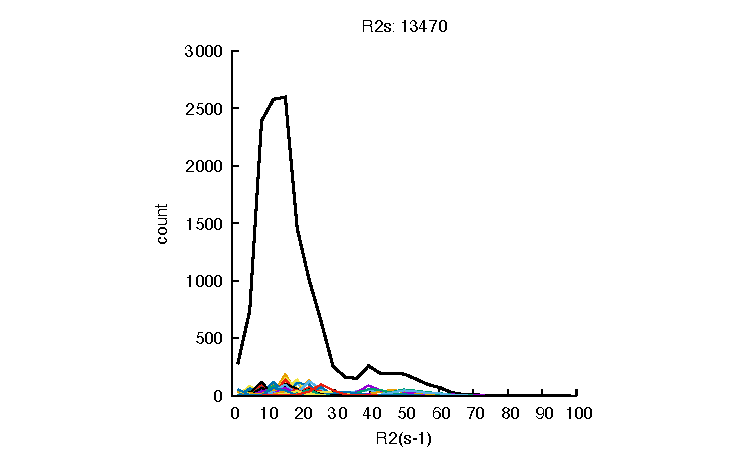
\includegraphics[trim= 3.000000cm 0.000000cm 3.000000cm 0.000000cm ,width=0.336700\textwidth]{R2fig.pdf}
\noindent 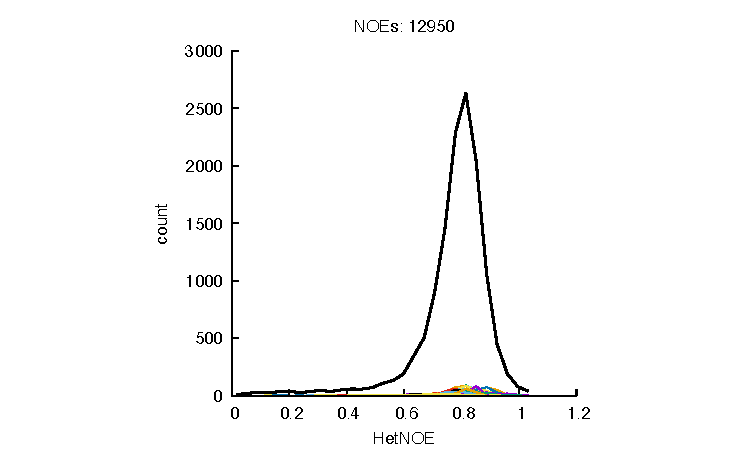
\includegraphics[trim= 3.000000cm 0.000000cm 3.000000cm 0.000000cm ,width=0.336700\textwidth]{NOEfig.pdf}
\noindent 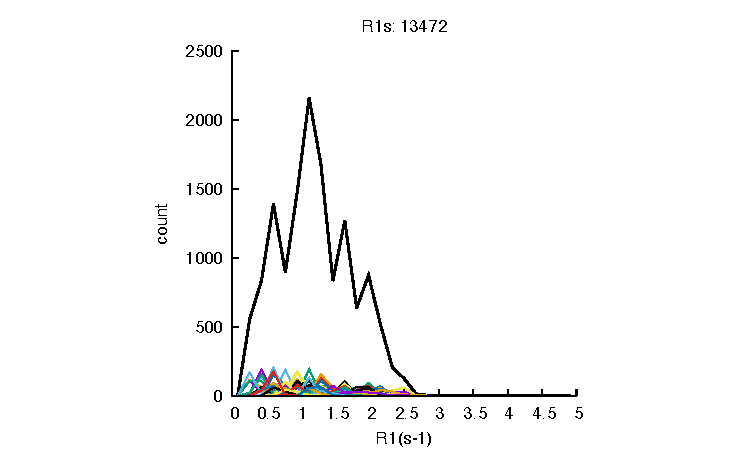
\includegraphics[trim= 3.000000cm 0.000000cm 3.000000cm 0.000000cm ,width=0.336700\textwidth]{R1fig.pdf}
\noindent 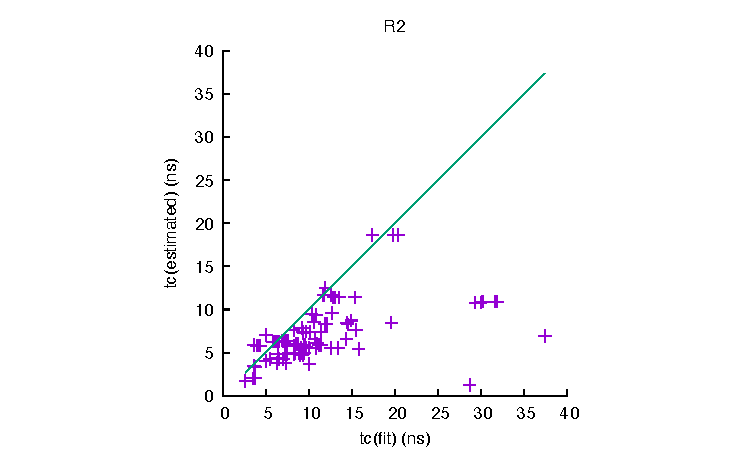
\includegraphics[trim= 3.000000cm 0.000000cm 3.000000cm 0.000000cm ,width=0.336700\textwidth]{tc1.pdf}
\noindent 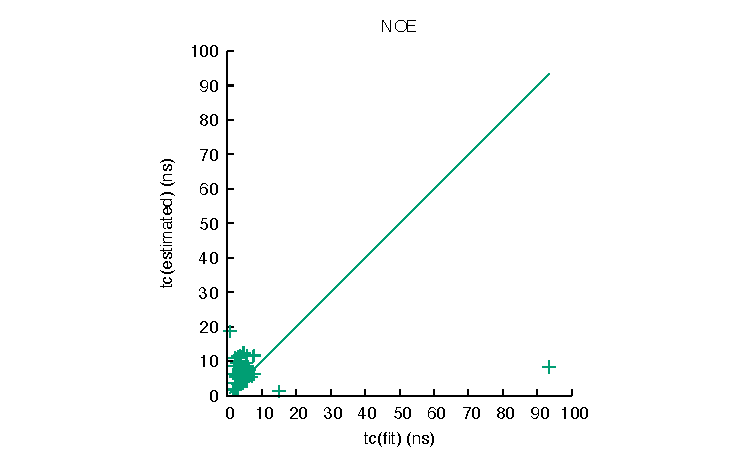
\includegraphics[trim= 3.000000cm 0.000000cm 3.000000cm 0.000000cm ,width=0.336700\textwidth]{tc2.pdf}
\noindent 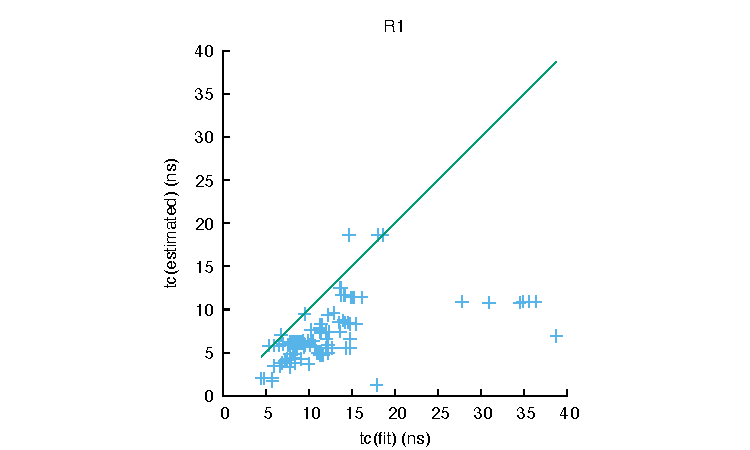
\includegraphics[trim= 3.000000cm 0.000000cm 3.000000cm 0.000000cm ,width=0.336700\textwidth]{tc3.pdf}
$\tau_c$ estimated from $\tau_c=\frac{\eta V}{k_b T}$. We can substitute for molecular weight and obtain $\tau_c=\frac{\eta}{\rho}\frac{M_w}{k_b T}$ where $M_w$ is in Da and $\rho$ is the density. The line takes the density to be water, and the viscosity to be 0.1 cP. The estimated value is compared to the fitted values from the three measurements.\clearpage

\begin{tiny}\noindent \begin{tabular}{lllllll}

\textbf{BMRB} & \textbf{Name} & \textbf{Fields}& \textbf{T} & \textbf{Residues} & \textbf{$M_w$ (kDa)} & \textbf{PDB}\\
\hline
bmr26710-bn & \verb|| & (2) 600,750& & & & \\
bmr26710-top & \verb|| & (1) 600& & & & \\
bmr26710-b2m & \verb|| & (1) 600& & & & \\
bmr5991 & \verb|Murine Ets-1 deltaN301| & (1) 500& 301& & & \\
bmr26507 & \verb|emagglutinin fusion peptide| & (1) 600& 305&  30& 3.15& \\
bmr50001 & \verb|ci-di-GMP in complex with ARR_CleD| & (1) 600& 298&  36& 4.16& \\
bmr18971 & \verb|WW3*-aENaC PY peptide complex| & (3) 600,799,899& 298&  43& 4.96& \\
bmr4390 & \verb|CC-chemokine eotaxin| & (1) 500& 303&  74& 8.36& \\
bmr4245 & \verb|ubiquitin| & (2) 500,600& 298&  76& 8.56& \\
bmr27011 & \verb|sigma1.1 monomer| & (3) 600,850,950& 298.2&  79& 9.38& 5MWW\\
bmr17069 & \verb|E73 Homodimer| & (1) 600& 312&  80& 9.58& \\
bmr15451 & \verb|OST domain in GABP alpha| & (1) 500& 298.0&  89& 9.97& \\
bmr11080 & \verb|CsPin| & (1) 500& 289&  97& 10.50& \\
bmr5079 & \verb|cytochrome c552| & (2) 500,600& 298&  100& 10.54& 1I6E\\
bmr5080 & \verb|cytochrome c552| & (2) 500,600& 298&  100& 10.54& 1I6D\\
bmr15437 & \verb|S836 monomer| & (2) 500,600& 298&  102& 11.93& \\
bmr5687 & \verb|protein S-824| & (2) 500,600& 298&  102& 11.93& \\
bmr18758 & \verb|First Catalytic Cysteine Half-domain| & (1) 400& 298&  112& 12.19& \\
bmr17010 & \verb|Tryptophan apo-repressor| & (1) 600& 318&  108& 12.36& 1WRT\\
bmr17013 & \verb|Tryptophan apo-repressor| & (1) 600& 318&  108& 12.38& 1WRT\\
bmr17012 & \verb|Tryptophan apo-repressor| & (1) 600& 318&  108& 12.39& 1WRT\\
bmr17041 & \verb|holoTrpR dimer| & (1) 600& 318&  113& 13.05& 1WRP\\
bmr17047 & \verb|holoTrpR dimer A77V variant| & (1) 600& 318&  113& 13.07& \\
bmr17046 & \verb|holoTrpR dimer L75F variant| & (1) 600& 318&  113& 13.08& 2XDI\\
bmr26506 & \verb|Rho-GTPase Binding Domain| & (1) 600& 298&  122& 13.44& 2JPH\\
bmr15562 & \verb|Ymr074cp (1-116) monomer| & (2) 600,500& 295&  127& 13.77& \\
bmr51417 & \verb|apo BD2  of BRD4| & (2) 600,800& 303&  120& 13.92& \\
bmr51414 & \verb|H4Kac bound BD2  of BRD4| & (2) 600,800& 303&  120, 16& 13.92& \\
bmr6243 & \verb|azurin| & (3) 500,600,800& 289&  128& 13.95& 4AZU\\
bmr5154 & \verb|NTD  MP1| & (1) 500& 293&  126& 14.25& 1D2B\\
bmr6577 & \verb|Bacillus stearothermophilus IF2-C1| & (1) 600& 307.4&  135& 14.80& \\
bmr51416 & \verb|apo BD1  of BRD4| & (2) 600,800& 303&  125& 14.86& \\
bmr51415 & \verb|H4Kac-bound BD1  of BRD4| & (2) 600,800& 303&  125, 16& 14.86& \\
bmr5841 & \verb|KAPP, kinase interaction domain| & (2) 500,600& 298&  139& 14.87& 1MZK\\
bmr6474 & \verb|KI-FHA domain of KAPP| & (2) 500,600& 295&  139& 14.87& 1MZK\\
bmr50284 & \verb|P-galectin3-C| & (3) 499,599,800& 301&  138& 15.68& 6RZH\\
bmr27722 & \verb|Gal3C R| & (3) 499,599,899& 301&  138& 15.68& \\
bmr27721 & \verb|Gal3C S| & (3) 499,599,899& 301&  138& 15.68& \\
bmr50283 & \verb|M-galectin3-C| & (3) 499,599,800& 301&  138& 15.68& 6RZG\\
bmr50285 & \verb|O-galectin3-C| & (3) 499,599,800& 301&  138& 15.68& 6RZF\\
bmr5330 & \verb|cellular retinol-binding protein type I| & (2) 500,600& 298&  135& 15.83& 1KGL\\
bmr5331 & \verb|cellular retinol-binding protein type I| & (2) 500,600& 298&  135& 15.83& 1KGL\\
bmr15445 & \verb|15.5K| & (2) 500,600& 293&  144& 16.00& \\
bmr4970 & \verb|Calmodulin| & (1) 500& 340&  148, 21& 16.71& \\
bmr19388 & \verb|MptpA| & (1) 600& 298&  164& 17.99& \\
bmr26513 & \verb|ligand-free MptpA| & (1) 600& 298&  167& 18.25& \\
bmr50212 & \verb|Mt-PPase| & (1) 700& 318&  162& 18.33& 4Z71\\
bmr4365 & \verb|stromelysin-ligand complexes| & (1) 600& 300&  166& 18.57& \\
bmr4364 & \verb|stromelysin-ligand complexes| & (1) 600& 300&  166& 18.57& \\
bmr4366 & \verb|stromelysin-ligand complexes| & (1) 600& 300&  166& 18.57& \\
bmr18389 & \verb|CtCBM11| & (1) 600& 323&  172& 18.94& \\
bmr18388 & \verb|CtCBM11| & (1) 600& 298&  172& 18.94& \\
bmr5153 & \verb|NTD  MP1/MMP3(E202Q)(deltaC) complex| & (1) 600& 307&  126, 173& 19.39& 1UEA\\
bmr27646 & \verb|KRas-G12C(1-169)-GDP| & (1) 700& 298&  171& 19.49& \\
bmr4267 & \verb|apo-HNGAL | & (3) 750,600,500& 298&  179& 20.68& 1NGL\\
bmr15230 & \verb|RalB-GMPPNP| & (1) 500& 298&  186& 21.11& \\
bmr18477 & \verb|A.fAglB_S2| & (2) 600,700& 308&  180& 21.17& \\
bmr4689 & \verb|Human Growth Hormone| & (1) 499& 305&  191& 22.13& \\
bmr25025 & \verb|NOX| & (2) 500,800& 323&  205& 22.75& 1NOX\\
bmr15097 & \verb|D6-HP| & (1) 750& 298&  208& 23.50& \\
bmr5746 & \verb|Adenylate Kinase from Escherichia coli| & (2) 600,800& 303&  214& 23.59& 1AKE\\
bmr26779 & \verb|Cdc25B monomer| & (1) 800& 298&  201& 23.72& 1QB0\\
bmr15066 & \verb|apo PGG/GGG| & (2) 600,800& 293&  248& 26.32& \\
bmr15065 & \verb|2-PGA bound WT cTIM homodimer| & (2) 600,800& 293&  248& 26.62& \\
bmr15064 & \verb|WT cTIM homodimer| & (2) 600,800& 293&  248& 26.62& 1TIM\\
bmr27888 & \verb|BlaC| & (2) 850,600& 298&  266& 28.30& 5NJ2\\
bmr27890 & \verb|BlaC in bound to clavulanic acid| & (1) 850& 298&  266& 28.30& 5NJ2\\
bmr27929 & \verb|BlaC bound to avibactam| & (1) 850& 298&  266& 28.30& 6H2H\\
bmr6838 & \verb|PSE-4| & (3) 500,600,800& 304.65&  271& 29.53& \\
bmr16392 & \verb|TEM-1| & (2) 500,600& 303.15&  286& 31.44& 1ERQ\\
bmr51413 & \verb|H4Kac bound BD1 , linker, BD2  of BRD4| & (2) 600,800& 303&  417, 16& 47.02& \\
bmr51418 & \verb|apo BD1 , linker, BD2  of BRD4| & (2) 600,800& 303&  417& 47.02& \\
\end{tabular}


\end{tiny}\clearpage

\section{Individual fits}

\noindent \subsection{bmr26710-bn: }

\begin{tabular}{ll}
\textbf{Fields:} &  600.2,750.5 MHz\\
\textbf{DataPts:} &  438\\
\end{tabular}

\begin{small}
\noindent \begin{tabular}{l|rlrl|rlrl}
& \multicolumn{4}{c}{600.18 MHz}& \multicolumn{4}{c}{750.46 MHz}\\
&  \multicolumn{2}{c}{rate} & \multicolumn{2}{c}{$\tau_c$ (ns)}   &  \multicolumn{2}{c}{rate} & \multicolumn{2}{c}{$\tau_c$ (ns)}   \\
\hline$R_2$  (s$^{-1}$)  &  25.888 & $\pm$ 2.380   &  18.45 & $\pm$ 1.79 &  28.482 & $\pm$ 1.997   &  18.03 & $\pm$ 1.75 \\
NOE  &  0.784 & $\pm$ 0.076   &  3.85 & $\pm$ 1.24 &  0.763 & $\pm$ 0.071   &  2.26 & $\pm$ 0.38 \\
$R_1$ (s$^{-1}$)  &  0.609 & $\pm$ 0.061   &  23.45 & $\pm$ 2.21 &  0.471 & $\pm$ 0.049   &  22.41 & $\pm$ 2.64 \\
$\sigma_{zz}$  (s$^{-1}$)  &  0.014 & $\pm$ 0.006   & & &  -0.000 & $\pm$ 0.009   & & \\
$\frac{R_1}{R_2}$  &  0.024 & $\pm$ 0.009   & & &  -0.003 & $\pm$ 0.011   & & \\
\end{tabular}
\end{small}


\noindent 
\includegraphics[trim= 3.000000cm 0.000000cm 3.000000cm 0.000000cm ,width=0.202020\textwidth]{bmr26710-bn/LocalTc.600.0.fig0.pdf}
\noindent 
\includegraphics[trim= 3.000000cm 0.000000cm 3.000000cm 0.000000cm ,width=0.202020\textwidth]{bmr26710-bn/LocalTc.600.0.fig1.pdf}
\noindent 
\includegraphics[trim= 3.000000cm 0.000000cm 3.000000cm 0.000000cm ,width=0.202020\textwidth]{bmr26710-bn/LocalTc.600.0.fig2.pdf}
\noindent 
\includegraphics[trim= 3.000000cm 0.000000cm 3.000000cm 0.000000cm ,width=0.202020\textwidth]{bmr26710-bn/LocalTc.600.0.fig3.pdf}
\noindent 
\includegraphics[trim= 3.000000cm 0.000000cm 3.000000cm 0.000000cm ,width=0.202020\textwidth]{bmr26710-bn/LocalTc.600.0.fig4.pdf}
\noindent 
\includegraphics[trim= 3.000000cm 0.000000cm 3.000000cm 0.000000cm ,width=0.202020\textwidth]{bmr26710-bn/LocalTc.600.18.fig0.pdf}
\noindent 
\includegraphics[trim= 3.000000cm 0.000000cm 3.000000cm 0.000000cm ,width=0.202020\textwidth]{bmr26710-bn/LocalTc.600.18.fig1.pdf}
\noindent 
\includegraphics[trim= 3.000000cm 0.000000cm 3.000000cm 0.000000cm ,width=0.202020\textwidth]{bmr26710-bn/LocalTc.600.18.fig2.pdf}
\noindent 
\includegraphics[trim= 3.000000cm 0.000000cm 3.000000cm 0.000000cm ,width=0.202020\textwidth]{bmr26710-bn/LocalTc.600.18.fig3.pdf}
\noindent 
\includegraphics[trim= 3.000000cm 0.000000cm 3.000000cm 0.000000cm ,width=0.202020\textwidth]{bmr26710-bn/LocalTc.600.18.fig4.pdf}
\noindent \subsection{bmr26710-top: }

\begin{tabular}{ll}
\textbf{Fields:} &  600.2 MHz\\
\textbf{DataPts:} &  321\\
\end{tabular}

\begin{small}
\noindent \begin{tabular}{l|rlrl}
& \multicolumn{4}{c}{600.18 MHz}\\
&  \multicolumn{2}{c}{rate} & \multicolumn{2}{c}{$\tau_c$ (ns)}   \\
\hline$R_2$  (s$^{-1}$)  &  25.750 & $\pm$ 2.585   &  18.37 & $\pm$ 1.89 \\
NOE  &  0.838 & $\pm$ 0.069   &  3.99 & $\pm$ 0.74 \\
$R_1$ (s$^{-1}$)  &  0.644 & $\pm$ 0.043   &  22.40 & $\pm$ 1.92 \\
$\sigma_{zz}$  (s$^{-1}$)  &  0.010 & $\pm$ 0.008   & & \\
$\frac{R_1}{R_2}$  &  0.014 & $\pm$ 0.008   & & \\
\end{tabular}
\end{small}


\noindent 
\includegraphics[trim= 3.000000cm 0.000000cm 3.000000cm 0.000000cm ,width=0.202020\textwidth]{bmr26710-top/LocalTc.800.0.fig0.pdf}
\noindent 
\includegraphics[trim= 3.000000cm 0.000000cm 3.000000cm 0.000000cm ,width=0.202020\textwidth]{bmr26710-top/LocalTc.800.0.fig1.pdf}
\noindent 
\includegraphics[trim= 3.000000cm 0.000000cm 3.000000cm 0.000000cm ,width=0.202020\textwidth]{bmr26710-top/LocalTc.800.0.fig2.pdf}
\noindent 
\includegraphics[trim= 3.000000cm 0.000000cm 3.000000cm 0.000000cm ,width=0.202020\textwidth]{bmr26710-top/LocalTc.800.0.fig3.pdf}
\noindent 
\includegraphics[trim= 3.000000cm 0.000000cm 3.000000cm 0.000000cm ,width=0.202020\textwidth]{bmr26710-top/LocalTc.800.0.fig4.pdf}
\noindent \subsection{bmr26710-b2m: }

\begin{tabular}{ll}
\textbf{Fields:} &  600.2 MHz\\
\textbf{DataPts:} &  165\\
\end{tabular}

\begin{small}
\noindent \begin{tabular}{l|rlrl}
& \multicolumn{4}{c}{600.18 MHz}\\
&  \multicolumn{2}{c}{rate} & \multicolumn{2}{c}{$\tau_c$ (ns)}   \\
\hline$R_2$  (s$^{-1}$)  &  24.442 & $\pm$ 1.501   &  17.62 & $\pm$ 1.42 \\
NOE  &  0.800 & $\pm$ 0.046   &  4.73 & $\pm$ 1.58 \\
$R_1$ (s$^{-1}$)  &  0.652 & $\pm$ 0.027   &  22.00 & $\pm$ 1.60 \\
$\sigma_{zz}$  (s$^{-1}$)  &  0.014 & $\pm$ 0.002   & & \\
$\frac{R_1}{R_2}$  &  0.030 & $\pm$ 0.002   & & \\
\end{tabular}
\end{small}


\noindent 
\includegraphics[trim= 3.000000cm 0.000000cm 3.000000cm 0.000000cm ,width=0.202020\textwidth]{bmr26710-b2m/LocalTc.500.0.fig0.pdf}
\noindent 
\includegraphics[trim= 3.000000cm 0.000000cm 3.000000cm 0.000000cm ,width=0.202020\textwidth]{bmr26710-b2m/LocalTc.500.0.fig1.pdf}
\noindent 
\includegraphics[trim= 3.000000cm 0.000000cm 3.000000cm 0.000000cm ,width=0.202020\textwidth]{bmr26710-b2m/LocalTc.500.0.fig2.pdf}
\noindent 
\includegraphics[trim= 3.000000cm 0.000000cm 3.000000cm 0.000000cm ,width=0.202020\textwidth]{bmr26710-b2m/LocalTc.500.0.fig3.pdf}
\noindent 
\includegraphics[trim= 3.000000cm 0.000000cm 3.000000cm 0.000000cm ,width=0.202020\textwidth]{bmr26710-b2m/LocalTc.500.0.fig4.pdf}
\noindent \subsection{bmr5991: Murine Ets-1 deltaN301}

\begin{tabular}{ll}
\textbf{Fields:} &  500.0 MHz\\
\textbf{DataPts:} &  375\\
 \textbf{T:} & 301 K\\
\end{tabular}

\begin{small}
\noindent \begin{tabular}{l|rlrl}
& \multicolumn{4}{c}{500.0 MHz}\\
&  \multicolumn{2}{c}{rate} & \multicolumn{2}{c}{$\tau_c$ (ns)}   \\
\hline$R_2$  (s$^{-1}$)  &  12.099 & $\pm$ 1.219   &  8.73 & $\pm$ 0.89 \\
NOE  &  0.738 & $\pm$ 0.105   &  3.70 & $\pm$ 1.05 \\
$R_1$ (s$^{-1}$)  &  1.687 & $\pm$ 0.077   &  10.59 & $\pm$ 0.72 \\
$\sigma_{zz}$  (s$^{-1}$)  &  0.052 & $\pm$ 0.014   & & \\
$\frac{R_1}{R_2}$  &  0.238 & $\pm$ 0.046   & & \\
\end{tabular}
\end{small}


\noindent 
\includegraphics[trim= 3.000000cm 0.000000cm 3.000000cm 0.000000cm ,width=0.202020\textwidth]{bmr5991/LocalTc.800.0.fig0.pdf}
\noindent 
\includegraphics[trim= 3.000000cm 0.000000cm 3.000000cm 0.000000cm ,width=0.202020\textwidth]{bmr5991/LocalTc.800.0.fig1.pdf}
\noindent 
\includegraphics[trim= 3.000000cm 0.000000cm 3.000000cm 0.000000cm ,width=0.202020\textwidth]{bmr5991/LocalTc.800.0.fig2.pdf}
\noindent 
\includegraphics[trim= 3.000000cm 0.000000cm 3.000000cm 0.000000cm ,width=0.202020\textwidth]{bmr5991/LocalTc.800.0.fig3.pdf}
\noindent 
\includegraphics[trim= 3.000000cm 0.000000cm 3.000000cm 0.000000cm ,width=0.202020\textwidth]{bmr5991/LocalTc.800.0.fig4.pdf}
\noindent \subsection{bmr26507: emagglutinin fusion peptide}

\begin{tabular}{ll}
\textbf{Fields:} &  600.0 MHz\\
\textbf{DataPts:} &  63\\
 \textbf{T:} & 305 K\\
\textbf{Mw:} & 3.15 kDa\\
\textbf{Residues: } &   30\\
\end{tabular}

\begin{small}
\noindent \begin{tabular}{l|rlrl}
& \multicolumn{4}{c}{600.0 MHz}\\
&  \multicolumn{2}{c}{rate} & \multicolumn{2}{c}{$\tau_c$ (ns)}   \\
\hline$R_2$  (s$^{-1}$)  &  39.521 & $\pm$ 0.965   &  28.67 & $\pm$ 2.96 \\
NOE  &  0.810 & $\pm$ 0.043   &  15.08 & $\pm$ 0.40 \\
$R_1$ (s$^{-1}$)  &  0.768 & $\pm$ 0.044   &  17.88 & $\pm$ 1.23 \\
$\sigma_{zz}$  (s$^{-1}$)  &  0.016 & $\pm$ 0.003   & & \\
$\frac{R_1}{R_2}$  &  0.018 & $\pm$ 0.002   & & \\
\end{tabular}
\end{small}


\noindent 
\includegraphics[trim= 3.000000cm 0.000000cm 3.000000cm 0.000000cm ,width=0.202020\textwidth]{bmr26507/LocalTc.600.0.fig0.pdf}
\noindent 
\includegraphics[trim= 3.000000cm 0.000000cm 3.000000cm 0.000000cm ,width=0.202020\textwidth]{bmr26507/LocalTc.600.0.fig1.pdf}
\noindent 
\includegraphics[trim= 3.000000cm 0.000000cm 3.000000cm 0.000000cm ,width=0.202020\textwidth]{bmr26507/LocalTc.600.0.fig2.pdf}
\noindent 
\includegraphics[trim= 3.000000cm 0.000000cm 3.000000cm 0.000000cm ,width=0.202020\textwidth]{bmr26507/LocalTc.600.0.fig3.pdf}
\noindent 
\includegraphics[trim= 3.000000cm 0.000000cm 3.000000cm 0.000000cm ,width=0.202020\textwidth]{bmr26507/LocalTc.600.0.fig4.pdf}
\noindent \subsection{bmr50001: ci-di-GMP in complex with ARR_CleD}

\begin{tabular}{ll}
\textbf{Fields:} &  600.1 MHz\\
\textbf{DataPts:} &  90\\
 \textbf{T:} & 298 K\\
\textbf{Mw:} & 4.16 kDa\\
\textbf{Residues: } &   36\\
\end{tabular}

\begin{small}
\noindent \begin{tabular}{l|rlrl}
& \multicolumn{4}{c}{600.12282197 MHz}\\
&  \multicolumn{2}{c}{rate} & \multicolumn{2}{c}{$\tau_c$ (ns)}   \\
\hline$R_2$  (s$^{-1}$)  &  5.045 & $\pm$ 0.952   &  2.65 & $\pm$ 0.71 \\
NOE  &  1.388 & $\pm$ 0.372   &  1.66 & $\pm$ 0.09 \\
$R_1$ (s$^{-1}$)  &  2.143 & $\pm$ 0.279   &  5.78 & $\pm$ 0.89 \\
$\sigma_{zz}$  (s$^{-1}$)  &  0.093 & $\pm$ 0.023   & & \\
$\frac{R_1}{R_2}$  &  0.109 & $\pm$ 0.055   & & \\
\end{tabular}
\end{small}


\noindent 
\includegraphics[trim= 3.000000cm 0.000000cm 3.000000cm 0.000000cm ,width=0.202020\textwidth]{bmr50001/LocalTc.800.0.fig0.pdf}
\noindent 
\includegraphics[trim= 3.000000cm 0.000000cm 3.000000cm 0.000000cm ,width=0.202020\textwidth]{bmr50001/LocalTc.800.0.fig1.pdf}
\noindent 
\includegraphics[trim= 3.000000cm 0.000000cm 3.000000cm 0.000000cm ,width=0.202020\textwidth]{bmr50001/LocalTc.800.0.fig2.pdf}
\noindent 
\includegraphics[trim= 3.000000cm 0.000000cm 3.000000cm 0.000000cm ,width=0.202020\textwidth]{bmr50001/LocalTc.800.0.fig3.pdf}
\noindent 
\includegraphics[trim= 3.000000cm 0.000000cm 3.000000cm 0.000000cm ,width=0.202020\textwidth]{bmr50001/LocalTc.800.0.fig4.pdf}
\noindent \subsection{bmr18971: WW3*-aENaC PY peptide complex}

\begin{tabular}{ll}
\textbf{Fields:} &  600.2,799.9,899.9 MHz\\
\textbf{DataPts:} &  306\\
 \textbf{T:} & 298 K\\
\textbf{Mw:} & 4.96 kDa\\
\textbf{Residues: } &   43\\
\end{tabular}

\begin{small}
\noindent \begin{tabular}{l|rlrl|rlrl|rlrl}
& \multicolumn{4}{c}{600.17 MHz}& \multicolumn{4}{c}{799.857 MHz}& \multicolumn{4}{c}{899.864 MHz}\\
&  \multicolumn{2}{c}{rate} & \multicolumn{2}{c}{$\tau_c$ (ns)}   &  \multicolumn{2}{c}{rate} & \multicolumn{2}{c}{$\tau_c$ (ns)}   &  \multicolumn{2}{c}{rate} & \multicolumn{2}{c}{$\tau_c$ (ns)}   \\
\hline$R_2$  (s$^{-1}$)  &  6.176 & $\pm$ 0.439   &  3.48 & $\pm$ 0.41 &  6.944 & $\pm$ 0.354   &  3.74 & $\pm$ 0.35 &  7.532 & $\pm$ 0.666   &  3.71 & $\pm$ 0.28 \\
NOE  &  0.813 & $\pm$ 0.072   &  3.02 & $\pm$ 0.25 &  1.734 & $\pm$ 0.220   &  2.67 & $\pm$ 0.37 &  0.824 & $\pm$ 0.029   &  2.27 & $\pm$ 0.30 \\
$R_1$ (s$^{-1}$)  &  2.194 & $\pm$ 0.131   &  5.74 & $\pm$ 0.36 &  1.719 & $\pm$ 0.075   &  4.79 & $\pm$ 0.31 &  1.603 & $\pm$ 0.046   &  4.51 & $\pm$ 0.15 \\
$\sigma_{zz}$  (s$^{-1}$)  &  0.062 & $\pm$ 0.004   & & &  0.037 & $\pm$ 0.001   & & &  0.033 & $\pm$ 0.003   & & \\
$\frac{R_1}{R_2}$  &  0.230 & $\pm$ 0.022   & & &  0.123 & $\pm$ 0.005   & & &  0.131 & $\pm$ 0.018   & & \\
\end{tabular}
\end{small}


\noindent 
\includegraphics[trim= 3.000000cm 0.000000cm 3.000000cm 0.000000cm ,width=0.202020\textwidth]{bmr18971/LocalTc.600.0.fig0.pdf}
\noindent 
\includegraphics[trim= 3.000000cm 0.000000cm 3.000000cm 0.000000cm ,width=0.202020\textwidth]{bmr18971/LocalTc.600.0.fig1.pdf}
\noindent 
\includegraphics[trim= 3.000000cm 0.000000cm 3.000000cm 0.000000cm ,width=0.202020\textwidth]{bmr18971/LocalTc.600.0.fig2.pdf}
\noindent 
\includegraphics[trim= 3.000000cm 0.000000cm 3.000000cm 0.000000cm ,width=0.202020\textwidth]{bmr18971/LocalTc.600.0.fig3.pdf}
\noindent 
\includegraphics[trim= 3.000000cm 0.000000cm 3.000000cm 0.000000cm ,width=0.202020\textwidth]{bmr18971/LocalTc.600.0.fig4.pdf}
\noindent 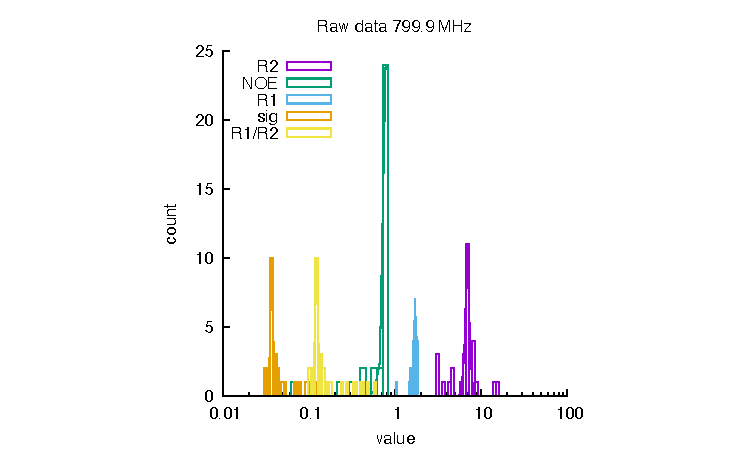
\includegraphics[trim= 3.000000cm 0.000000cm 3.000000cm 0.000000cm ,width=0.202020\textwidth]{bmr18971/LocalTc.600.17.fig0.pdf}
\noindent 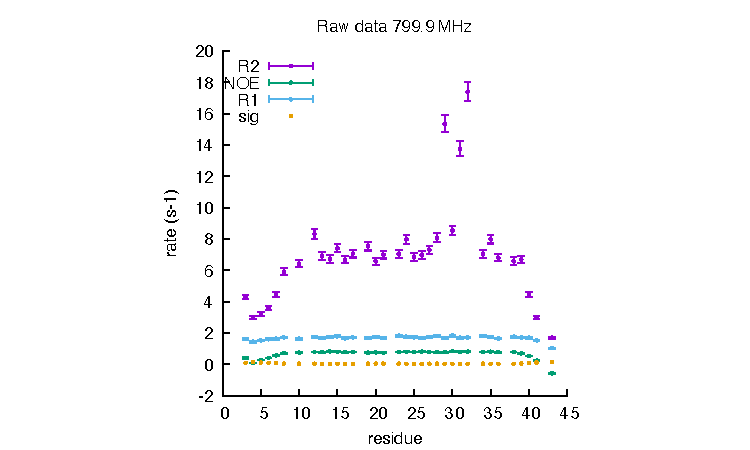
\includegraphics[trim= 3.000000cm 0.000000cm 3.000000cm 0.000000cm ,width=0.202020\textwidth]{bmr18971/LocalTc.600.17.fig1.pdf}
\noindent 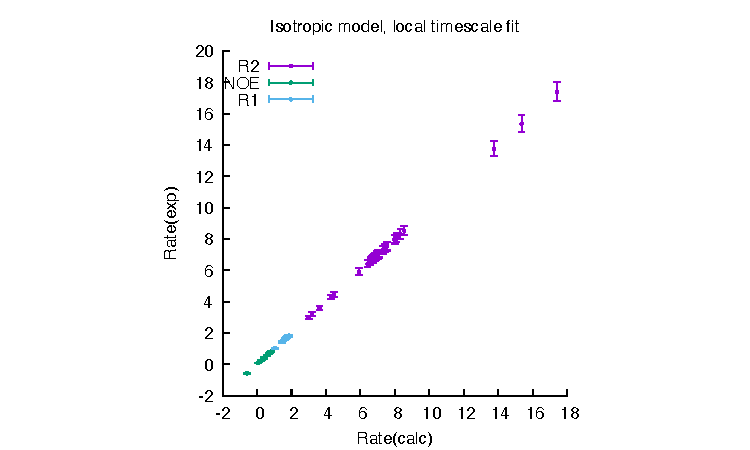
\includegraphics[trim= 3.000000cm 0.000000cm 3.000000cm 0.000000cm ,width=0.202020\textwidth]{bmr18971/LocalTc.600.17.fig2.pdf}
\noindent 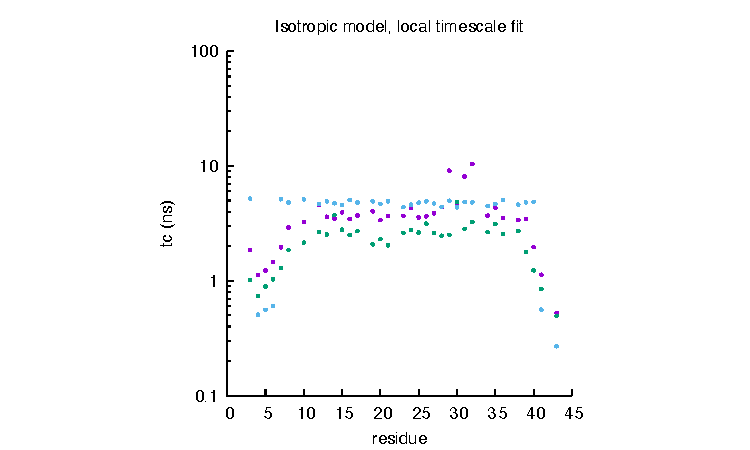
\includegraphics[trim= 3.000000cm 0.000000cm 3.000000cm 0.000000cm ,width=0.202020\textwidth]{bmr18971/LocalTc.600.17.fig3.pdf}
\noindent 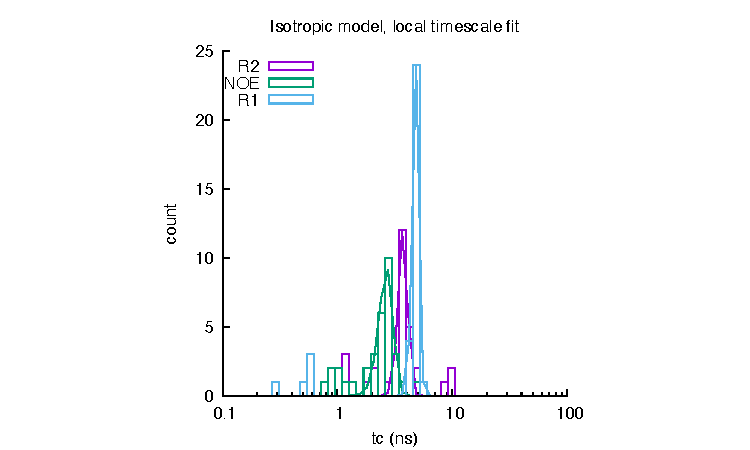
\includegraphics[trim= 3.000000cm 0.000000cm 3.000000cm 0.000000cm ,width=0.202020\textwidth]{bmr18971/LocalTc.600.17.fig4.pdf}
\noindent 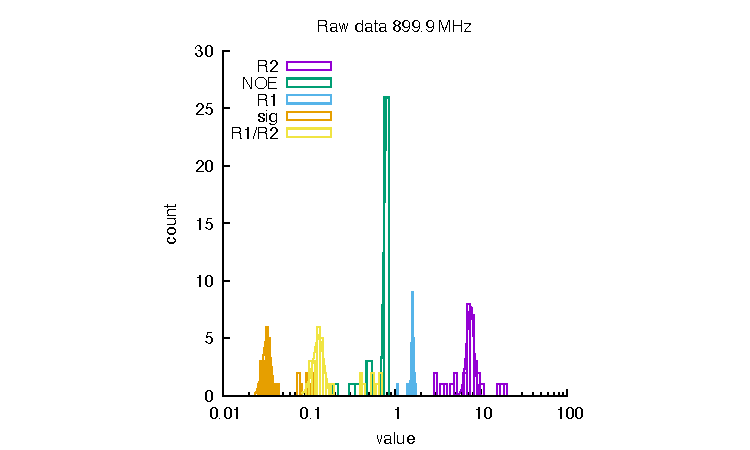
\includegraphics[trim= 3.000000cm 0.000000cm 3.000000cm 0.000000cm ,width=0.202020\textwidth]{bmr18971/LocalTc.799.857.fig0.pdf}
\noindent 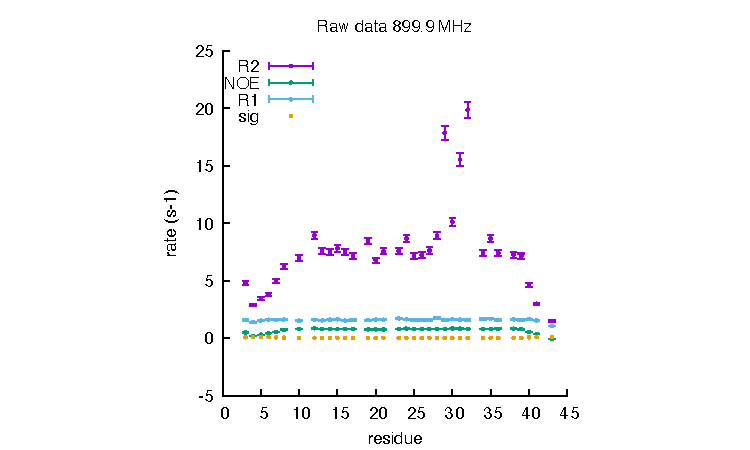
\includegraphics[trim= 3.000000cm 0.000000cm 3.000000cm 0.000000cm ,width=0.202020\textwidth]{bmr18971/LocalTc.799.857.fig1.pdf}
\noindent 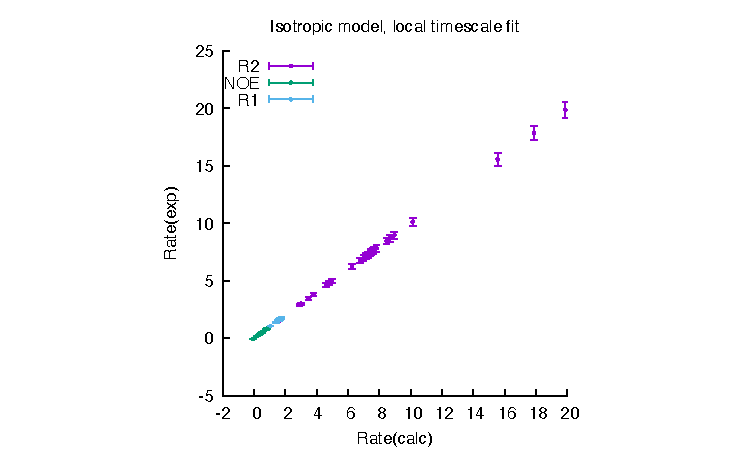
\includegraphics[trim= 3.000000cm 0.000000cm 3.000000cm 0.000000cm ,width=0.202020\textwidth]{bmr18971/LocalTc.799.857.fig2.pdf}
\noindent 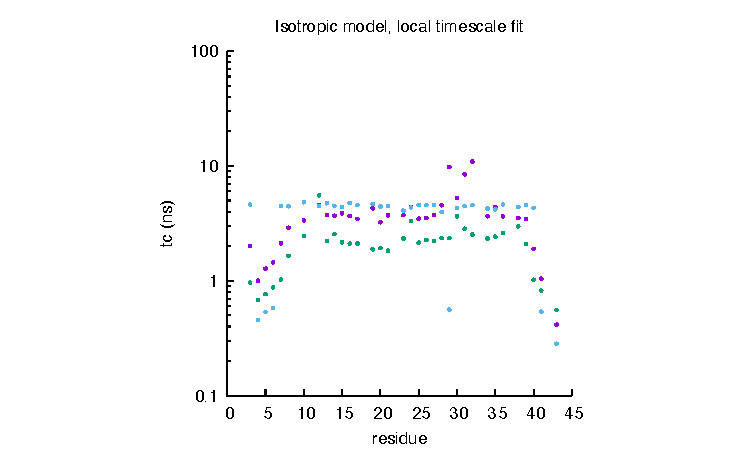
\includegraphics[trim= 3.000000cm 0.000000cm 3.000000cm 0.000000cm ,width=0.202020\textwidth]{bmr18971/LocalTc.799.857.fig3.pdf}
\noindent 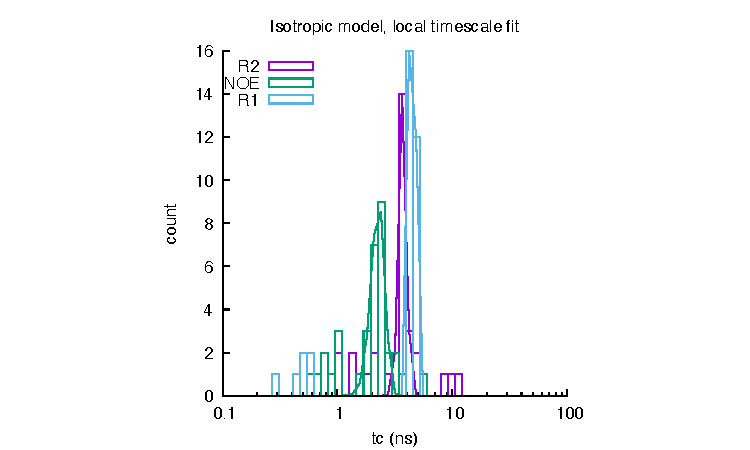
\includegraphics[trim= 3.000000cm 0.000000cm 3.000000cm 0.000000cm ,width=0.202020\textwidth]{bmr18971/LocalTc.799.857.fig4.pdf}
\noindent \subsection{bmr4390: CC-chemokine eotaxin}

\begin{tabular}{ll}
\textbf{Fields:} &  500.0 MHz\\
\textbf{DataPts:} &  171\\
 \textbf{T:} & 303 K\\
\textbf{Mw:} & 8.36 kDa\\
\textbf{Residues: } &   74\\
\end{tabular}

\begin{small}
\noindent \begin{tabular}{l|rlrl}
& \multicolumn{4}{c}{500.0 MHz}\\
&  \multicolumn{2}{c}{rate} & \multicolumn{2}{c}{$\tau_c$ (ns)}   \\
\hline$R_2$  (s$^{-1}$)  &  6.330 & $\pm$ 0.353   &  3.77 & $\pm$ 0.29 \\
NOE  &  0.683 & $\pm$ 0.100   &  3.11 & $\pm$ 0.42 \\
$R_1$ (s$^{-1}$)  &  2.161 & $\pm$ 0.158   &  7.79 & $\pm$ 0.78 \\
$\sigma_{zz}$  (s$^{-1}$)  &  0.080 & $\pm$ 0.009   & & \\
$\frac{R_1}{R_2}$  &  0.236 & $\pm$ 0.028   & & \\
\end{tabular}
\end{small}


\noindent 
\includegraphics[trim= 3.000000cm 0.000000cm 3.000000cm 0.000000cm ,width=0.202020\textwidth]{bmr4390/LocalTc.600.0.fig0.pdf}
\noindent 
\includegraphics[trim= 3.000000cm 0.000000cm 3.000000cm 0.000000cm ,width=0.202020\textwidth]{bmr4390/LocalTc.600.0.fig1.pdf}
\noindent 
\includegraphics[trim= 3.000000cm 0.000000cm 3.000000cm 0.000000cm ,width=0.202020\textwidth]{bmr4390/LocalTc.600.0.fig2.pdf}
\noindent 
\includegraphics[trim= 3.000000cm 0.000000cm 3.000000cm 0.000000cm ,width=0.202020\textwidth]{bmr4390/LocalTc.600.0.fig3.pdf}
\noindent 
\includegraphics[trim= 3.000000cm 0.000000cm 3.000000cm 0.000000cm ,width=0.202020\textwidth]{bmr4390/LocalTc.600.0.fig4.pdf}
\noindent \subsection{bmr4245: ubiquitin}

\begin{tabular}{ll}
\textbf{Fields:} &  500.0,600.0 MHz\\
\textbf{DataPts:} &  372\\
 \textbf{T:} & 298 K\\
\textbf{Mw:} & 8.56 kDa\\
\textbf{Residues: } &   76\\
\end{tabular}

\begin{small}
\noindent \begin{tabular}{l|rlrl|rlrl}
& \multicolumn{4}{c}{500.0 MHz}& \multicolumn{4}{c}{600.0 MHz}\\
&  \multicolumn{2}{c}{rate} & \multicolumn{2}{c}{$\tau_c$ (ns)}   &  \multicolumn{2}{c}{rate} & \multicolumn{2}{c}{$\tau_c$ (ns)}   \\
\hline$R_2$  (s$^{-1}$)  &  6.198 & $\pm$ 0.269   &  3.61 & $\pm$ 0.30 &  6.404 & $\pm$ 0.291   &  3.64 & $\pm$ 0.26 \\
NOE  &  1.391 & $\pm$ 0.178   &  4.03 & $\pm$ 0.61 &  1.348 & $\pm$ 0.179   &  4.12 & $\pm$ 0.82 \\
$R_1$ (s$^{-1}$)  &  2.434 & $\pm$ 0.104   &  6.65 & $\pm$ 0.46 &  2.070 & $\pm$ 0.069   &  5.95 & $\pm$ 0.25 \\
$\sigma_{zz}$  (s$^{-1}$)  &  0.071 & $\pm$ 0.009   & & &  0.049 & $\pm$ 0.005   & & \\
$\frac{R_1}{R_2}$  &  0.347 & $\pm$ 0.033   & & &  0.261 & $\pm$ 0.019   & & \\
\end{tabular}
\end{small}


\noindent 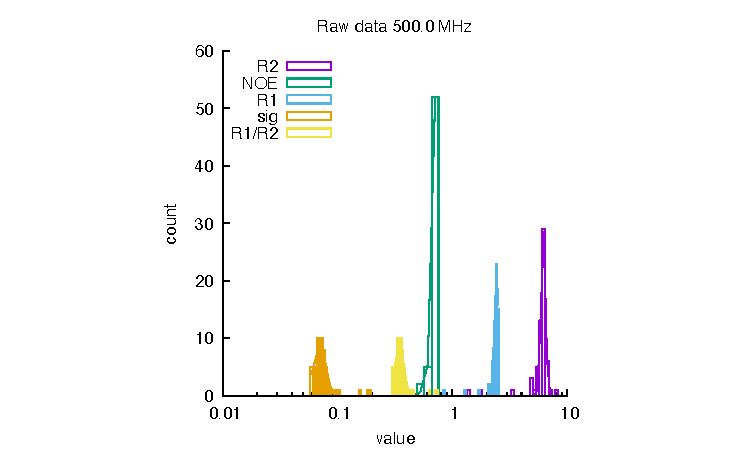
\includegraphics[trim= 3.000000cm 0.000000cm 3.000000cm 0.000000cm ,width=0.202020\textwidth]{bmr4245/LocalTc.500.13.fig0.pdf}
\noindent 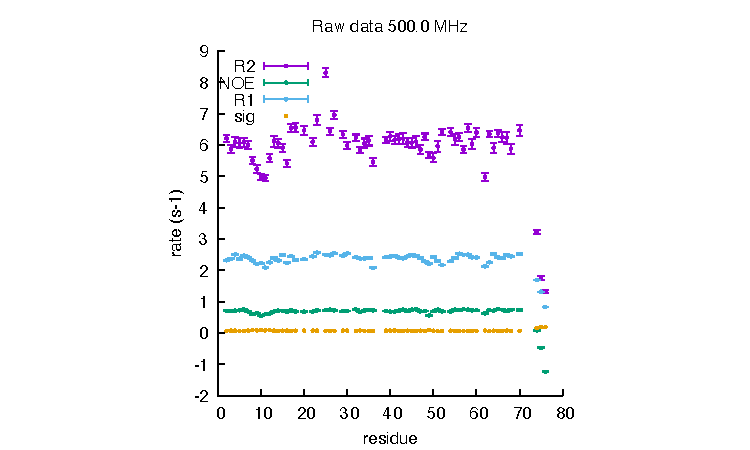
\includegraphics[trim= 3.000000cm 0.000000cm 3.000000cm 0.000000cm ,width=0.202020\textwidth]{bmr4245/LocalTc.500.13.fig1.pdf}
\noindent 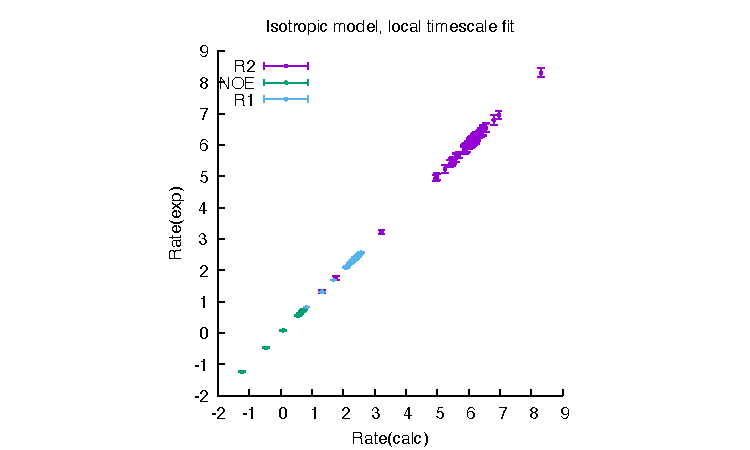
\includegraphics[trim= 3.000000cm 0.000000cm 3.000000cm 0.000000cm ,width=0.202020\textwidth]{bmr4245/LocalTc.500.13.fig2.pdf}
\noindent 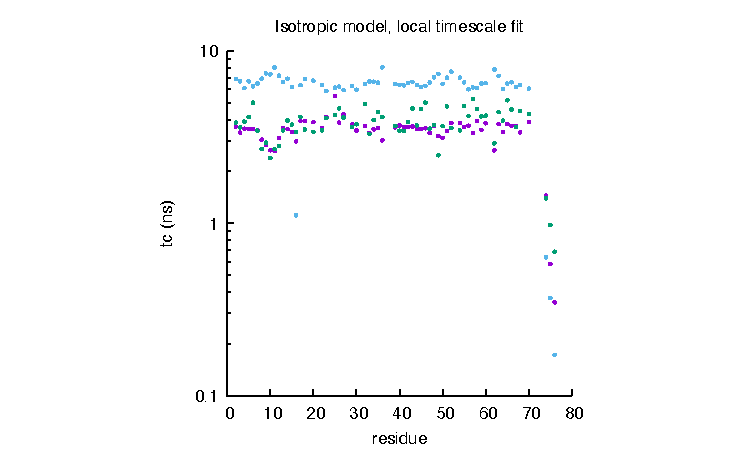
\includegraphics[trim= 3.000000cm 0.000000cm 3.000000cm 0.000000cm ,width=0.202020\textwidth]{bmr4245/LocalTc.500.13.fig3.pdf}
\noindent 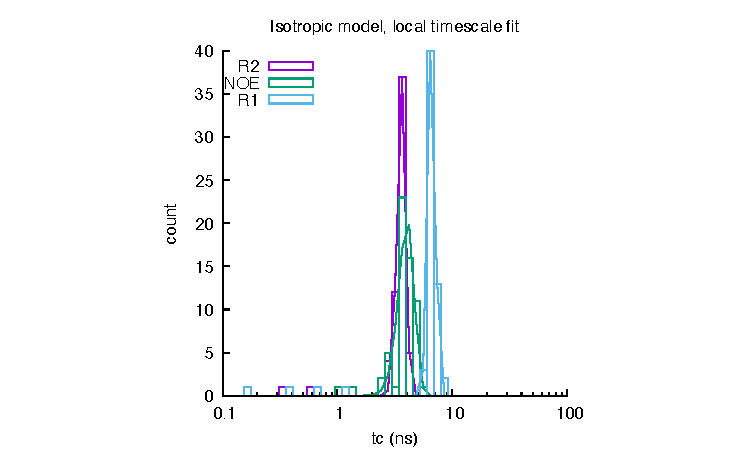
\includegraphics[trim= 3.000000cm 0.000000cm 3.000000cm 0.000000cm ,width=0.202020\textwidth]{bmr4245/LocalTc.500.13.fig4.pdf}
\noindent 
\includegraphics[trim= 3.000000cm 0.000000cm 3.000000cm 0.000000cm ,width=0.202020\textwidth]{bmr4245/LocalTc.500.0.fig0.pdf}
\noindent 
\includegraphics[trim= 3.000000cm 0.000000cm 3.000000cm 0.000000cm ,width=0.202020\textwidth]{bmr4245/LocalTc.500.0.fig1.pdf}
\noindent 
\includegraphics[trim= 3.000000cm 0.000000cm 3.000000cm 0.000000cm ,width=0.202020\textwidth]{bmr4245/LocalTc.500.0.fig2.pdf}
\noindent 
\includegraphics[trim= 3.000000cm 0.000000cm 3.000000cm 0.000000cm ,width=0.202020\textwidth]{bmr4245/LocalTc.500.0.fig3.pdf}
\noindent 
\includegraphics[trim= 3.000000cm 0.000000cm 3.000000cm 0.000000cm ,width=0.202020\textwidth]{bmr4245/LocalTc.500.0.fig4.pdf}
\noindent \subsection{bmr27011: sigma1.1 monomer}

\begin{tabular}{ll}
\textbf{Fields:} &  600.0,850.0,950.0 MHz\\
\textbf{DataPts:} &  576\\
 \textbf{T:} & 298.2 K\\
\textbf{Mw:} & 9.38 kDa\\
\textbf{Residues: } &   79\\
\end{tabular}

\begin{small}
\noindent \begin{tabular}{l|rlrl|rlrl|rlrl}
& \multicolumn{4}{c}{600.0 MHz}& \multicolumn{4}{c}{850.0 MHz}& \multicolumn{4}{c}{950.0 MHz}\\
&  \multicolumn{2}{c}{rate} & \multicolumn{2}{c}{$\tau_c$ (ns)}   &  \multicolumn{2}{c}{rate} & \multicolumn{2}{c}{$\tau_c$ (ns)}   &  \multicolumn{2}{c}{rate} & \multicolumn{2}{c}{$\tau_c$ (ns)}   \\
\hline$R_2$  (s$^{-1}$)  &  9.650 & $\pm$ 1.642   &  6.32 & $\pm$ 1.12 &  9.650 & $\pm$ 1.642   &  6.32 & $\pm$ 1.12 &  13.871 & $\pm$ 3.147   &  7.32 & $\pm$ 2.00 \\
NOE  &  0.724 & $\pm$ 0.049   &  3.00 & $\pm$ 0.40 &  0.724 & $\pm$ 0.049   &  3.00 & $\pm$ 0.40 &  3.767 & $\pm$ 0.555   &  2.26 & $\pm$ 0.78 \\
$R_1$ (s$^{-1}$)  &  1.617 & $\pm$ 0.085   &  8.39 & $\pm$ 0.72 &  1.617 & $\pm$ 0.085   &  8.39 & $\pm$ 0.72 &  1.077 & $\pm$ 0.061   &  6.88 & $\pm$ 0.63 \\
$\sigma_{zz}$  (s$^{-1}$)  &  0.047 & $\pm$ 0.006   & & &  0.047 & $\pm$ 0.006   & & &  0.021 & $\pm$ 0.004   & & \\
$\frac{R_1}{R_2}$  &  0.172 & $\pm$ 0.018   & & &  0.172 & $\pm$ 0.018   & & &  0.084 & $\pm$ 0.020   & & \\
\end{tabular}
\end{small}


\noindent 
\includegraphics[trim= 3.000000cm 0.000000cm 3.000000cm 0.000000cm ,width=0.202020\textwidth]{bmr27011/LocalTc.600.0.fig0.pdf}
\noindent 
\includegraphics[trim= 3.000000cm 0.000000cm 3.000000cm 0.000000cm ,width=0.202020\textwidth]{bmr27011/LocalTc.600.0.fig1.pdf}
\noindent 
\includegraphics[trim= 3.000000cm 0.000000cm 3.000000cm 0.000000cm ,width=0.202020\textwidth]{bmr27011/LocalTc.600.0.fig2.pdf}
\noindent 
\includegraphics[trim= 3.000000cm 0.000000cm 3.000000cm 0.000000cm ,width=0.202020\textwidth]{bmr27011/LocalTc.600.0.fig3.pdf}
\noindent 
\includegraphics[trim= 3.000000cm 0.000000cm 3.000000cm 0.000000cm ,width=0.202020\textwidth]{bmr27011/LocalTc.600.0.fig4.pdf}
\noindent 
\includegraphics[trim= 3.000000cm 0.000000cm 3.000000cm 0.000000cm ,width=0.202020\textwidth]{bmr27011/LocalTc.600.0.fig0.pdf}
\noindent 
\includegraphics[trim= 3.000000cm 0.000000cm 3.000000cm 0.000000cm ,width=0.202020\textwidth]{bmr27011/LocalTc.600.0.fig1.pdf}
\noindent 
\includegraphics[trim= 3.000000cm 0.000000cm 3.000000cm 0.000000cm ,width=0.202020\textwidth]{bmr27011/LocalTc.600.0.fig2.pdf}
\noindent 
\includegraphics[trim= 3.000000cm 0.000000cm 3.000000cm 0.000000cm ,width=0.202020\textwidth]{bmr27011/LocalTc.600.0.fig3.pdf}
\noindent 
\includegraphics[trim= 3.000000cm 0.000000cm 3.000000cm 0.000000cm ,width=0.202020\textwidth]{bmr27011/LocalTc.600.0.fig4.pdf}
\noindent 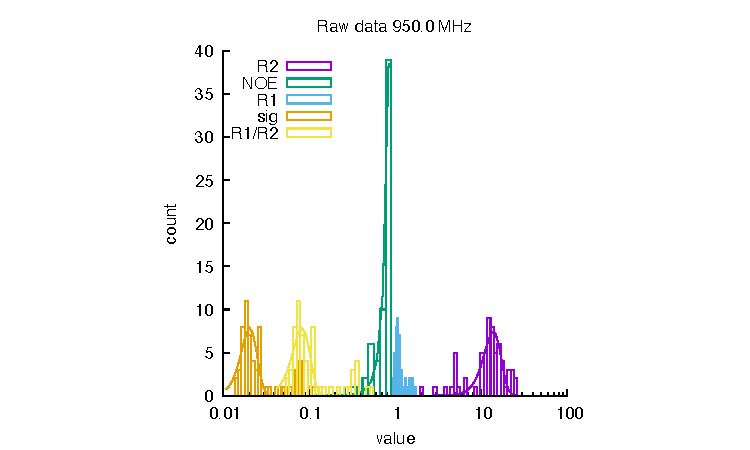
\includegraphics[trim= 3.000000cm 0.000000cm 3.000000cm 0.000000cm ,width=0.202020\textwidth]{bmr27011/LocalTc.850.0.fig0.pdf}
\noindent 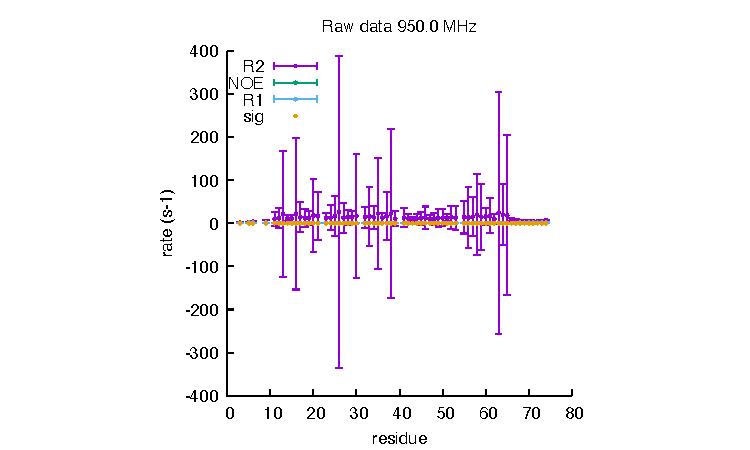
\includegraphics[trim= 3.000000cm 0.000000cm 3.000000cm 0.000000cm ,width=0.202020\textwidth]{bmr27011/LocalTc.850.0.fig1.pdf}
\noindent 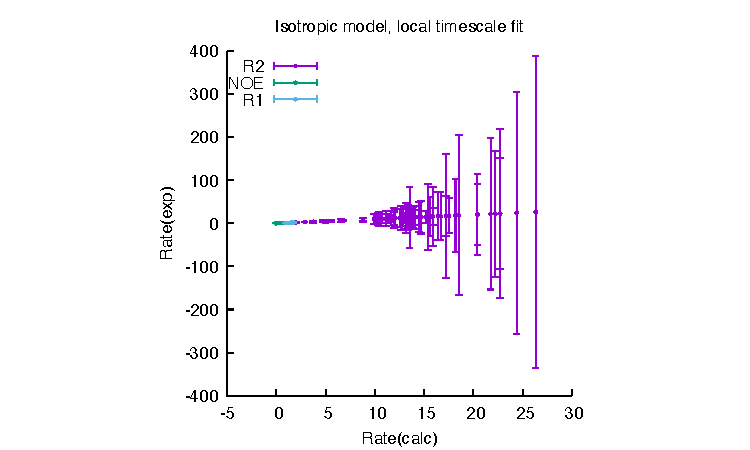
\includegraphics[trim= 3.000000cm 0.000000cm 3.000000cm 0.000000cm ,width=0.202020\textwidth]{bmr27011/LocalTc.850.0.fig2.pdf}
\noindent 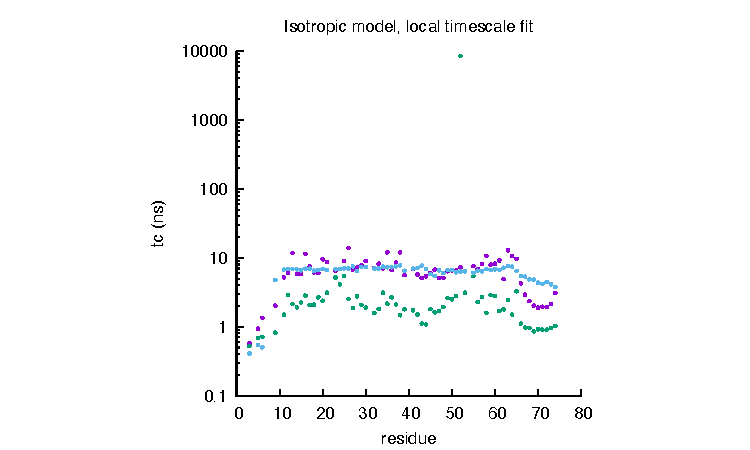
\includegraphics[trim= 3.000000cm 0.000000cm 3.000000cm 0.000000cm ,width=0.202020\textwidth]{bmr27011/LocalTc.850.0.fig3.pdf}
\noindent 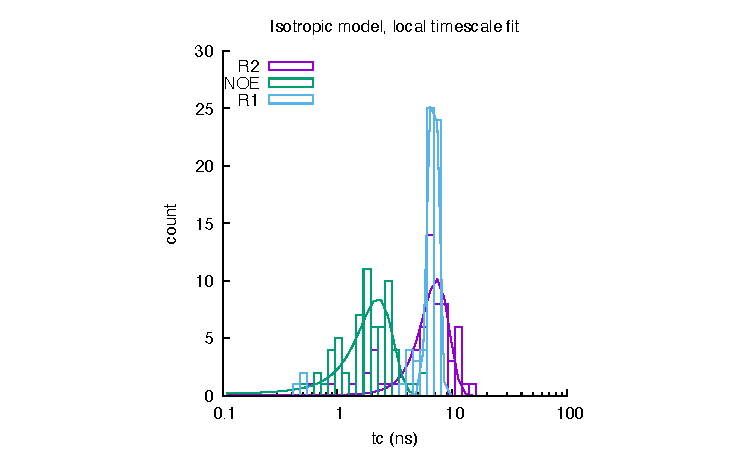
\includegraphics[trim= 3.000000cm 0.000000cm 3.000000cm 0.000000cm ,width=0.202020\textwidth]{bmr27011/LocalTc.850.0.fig4.pdf}
\noindent \subsection{bmr17069: E73 Homodimer}

\begin{tabular}{ll}
\textbf{Fields:} &  600.0 MHz\\
\textbf{DataPts:} &  174\\
 \textbf{T:} & 312 K\\
\textbf{Mw:} & 9.58 kDa\\
\textbf{Residues: } &   80\\
\end{tabular}

\begin{small}
\noindent \begin{tabular}{l|rlrl}
& \multicolumn{4}{c}{600.0 MHz}\\
&  \multicolumn{2}{c}{rate} & \multicolumn{2}{c}{$\tau_c$ (ns)}   \\
\hline$R_2$  (s$^{-1}$)  &  14.554 & $\pm$ 1.271   &  10.06 & $\pm$ 0.79 \\
NOE  &  0.776 & $\pm$ 0.076   &  3.62 & $\pm$ 0.90 \\
$R_1$ (s$^{-1}$)  &  1.364 & $\pm$ 0.074   &  9.97 & $\pm$ 0.71 \\
$\sigma_{zz}$  (s$^{-1}$)  &  0.035 & $\pm$ 0.008   & & \\
$\frac{R_1}{R_2}$  &  0.099 & $\pm$ 0.021   & & \\
\end{tabular}
\end{small}


\noindent 
\includegraphics[trim= 3.000000cm 0.000000cm 3.000000cm 0.000000cm ,width=0.202020\textwidth]{bmr17069/LocalTc.600.0.fig0.pdf}
\noindent 
\includegraphics[trim= 3.000000cm 0.000000cm 3.000000cm 0.000000cm ,width=0.202020\textwidth]{bmr17069/LocalTc.600.0.fig1.pdf}
\noindent 
\includegraphics[trim= 3.000000cm 0.000000cm 3.000000cm 0.000000cm ,width=0.202020\textwidth]{bmr17069/LocalTc.600.0.fig2.pdf}
\noindent 
\includegraphics[trim= 3.000000cm 0.000000cm 3.000000cm 0.000000cm ,width=0.202020\textwidth]{bmr17069/LocalTc.600.0.fig3.pdf}
\noindent 
\includegraphics[trim= 3.000000cm 0.000000cm 3.000000cm 0.000000cm ,width=0.202020\textwidth]{bmr17069/LocalTc.600.0.fig4.pdf}
\noindent \subsection{bmr15451: OST domain in GABP alpha}

\begin{tabular}{ll}
\textbf{Fields:} &  500.0 MHz\\
\textbf{DataPts:} &  231\\
 \textbf{T:} & 298.0 K\\
\textbf{Mw:} & 9.97 kDa\\
\textbf{Residues: } &   89\\
\end{tabular}

\begin{small}
\noindent \begin{tabular}{l|rlrl}
& \multicolumn{4}{c}{500.0 MHz}\\
&  \multicolumn{2}{c}{rate} & \multicolumn{2}{c}{$\tau_c$ (ns)}   \\
\hline$R_2$  (s$^{-1}$)  &  7.776 & $\pm$ 0.452   &  4.99 & $\pm$ 0.45 \\
NOE  &  0.770 & $\pm$ 0.087   &  4.66 & $\pm$ 1.22 \\
$R_1$ (s$^{-1}$)  &  2.287 & $\pm$ 0.144   &  7.23 & $\pm$ 0.79 \\
$\sigma_{zz}$  (s$^{-1}$)  &  0.061 & $\pm$ 0.008   & & \\
$\frac{R_1}{R_2}$  &  0.216 & $\pm$ 0.011   & & \\
\end{tabular}
\end{small}


\noindent 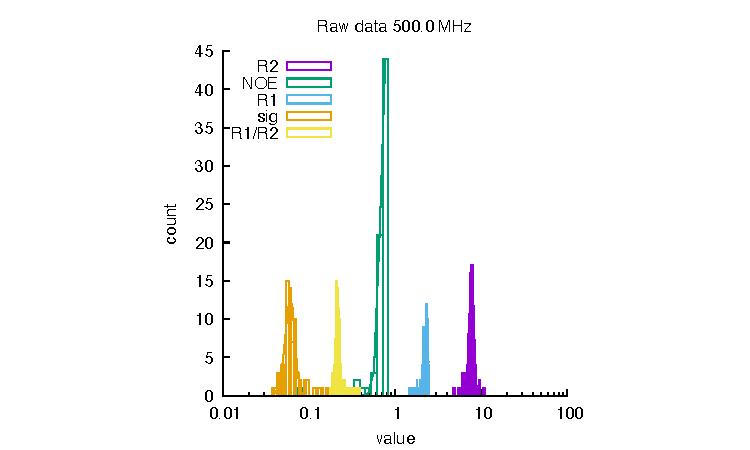
\includegraphics[trim= 3.000000cm 0.000000cm 3.000000cm 0.000000cm ,width=0.202020\textwidth]{bmr15451/LocalTc.899.864.fig0.pdf}
\noindent 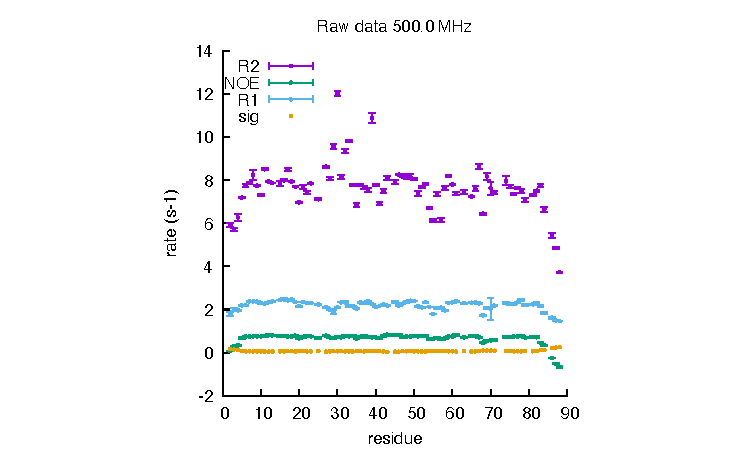
\includegraphics[trim= 3.000000cm 0.000000cm 3.000000cm 0.000000cm ,width=0.202020\textwidth]{bmr15451/LocalTc.899.864.fig1.pdf}
\noindent 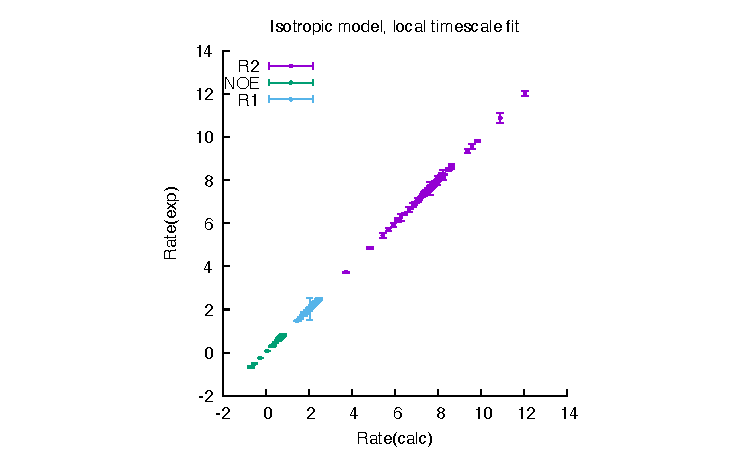
\includegraphics[trim= 3.000000cm 0.000000cm 3.000000cm 0.000000cm ,width=0.202020\textwidth]{bmr15451/LocalTc.899.864.fig2.pdf}
\noindent 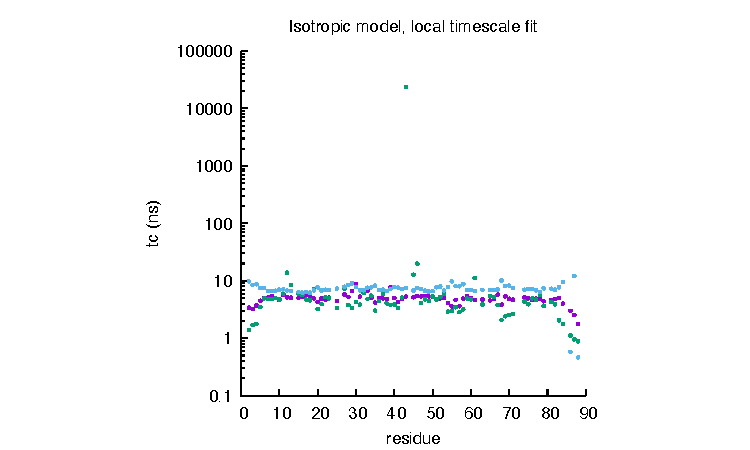
\includegraphics[trim= 3.000000cm 0.000000cm 3.000000cm 0.000000cm ,width=0.202020\textwidth]{bmr15451/LocalTc.899.864.fig3.pdf}
\noindent 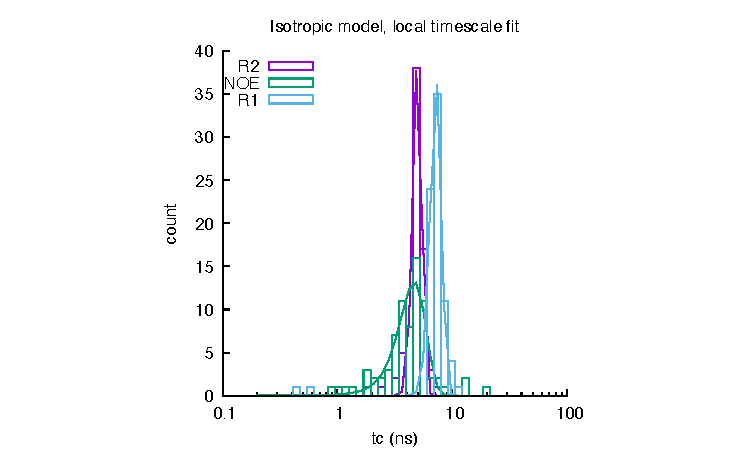
\includegraphics[trim= 3.000000cm 0.000000cm 3.000000cm 0.000000cm ,width=0.202020\textwidth]{bmr15451/LocalTc.899.864.fig4.pdf}
\noindent \subsection{bmr11080: CsPin}

\begin{tabular}{ll}
\textbf{Fields:} &  500.0 MHz\\
\textbf{DataPts:} &  222\\
 \textbf{T:} & 289 K\\
\textbf{Mw:} & 10.50 kDa\\
\textbf{Residues: } &   97\\
\end{tabular}

\begin{small}
\noindent \begin{tabular}{l|rlrl}
& \multicolumn{4}{c}{500.0 MHz}\\
&  \multicolumn{2}{c}{rate} & \multicolumn{2}{c}{$\tau_c$ (ns)}   \\
\hline$R_2$  (s$^{-1}$)  &  9.367 & $\pm$ 0.413   &  6.40 & $\pm$ 0.47 \\
NOE  &  0.762 & $\pm$ 0.071   &  4.53 & $\pm$ 1.27 \\
$R_1$ (s$^{-1}$)  &  2.052 & $\pm$ 0.073   &  8.38 & $\pm$ 0.62 \\
$\sigma_{zz}$  (s$^{-1}$)  &  0.055 & $\pm$ 0.014   & & \\
$\frac{R_1}{R_2}$  &  0.240 & $\pm$ 0.010   & & \\
\end{tabular}
\end{small}


\noindent 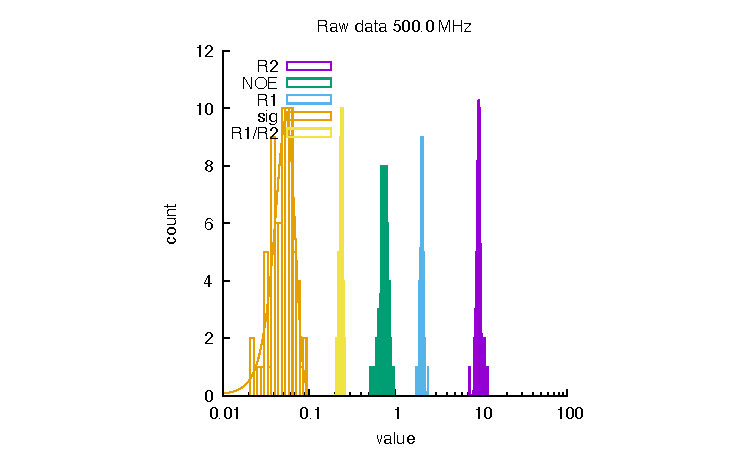
\includegraphics[trim= 3.000000cm 0.000000cm 3.000000cm 0.000000cm ,width=0.202020\textwidth]{bmr11080/LocalTc.600.0.fig0.pdf}
\noindent 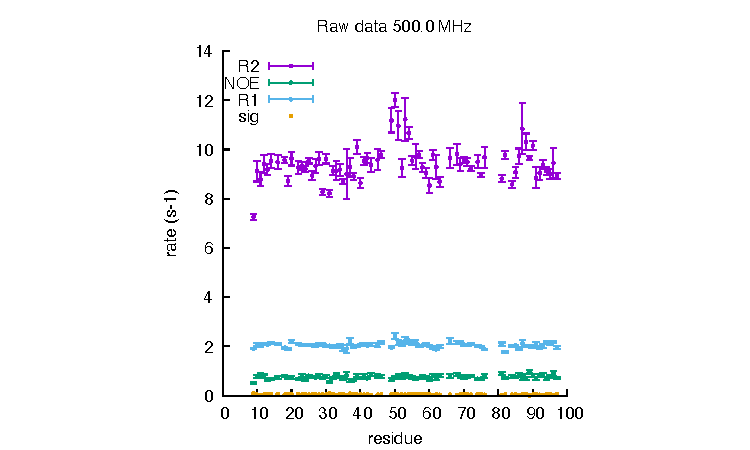
\includegraphics[trim= 3.000000cm 0.000000cm 3.000000cm 0.000000cm ,width=0.202020\textwidth]{bmr11080/LocalTc.600.0.fig1.pdf}
\noindent 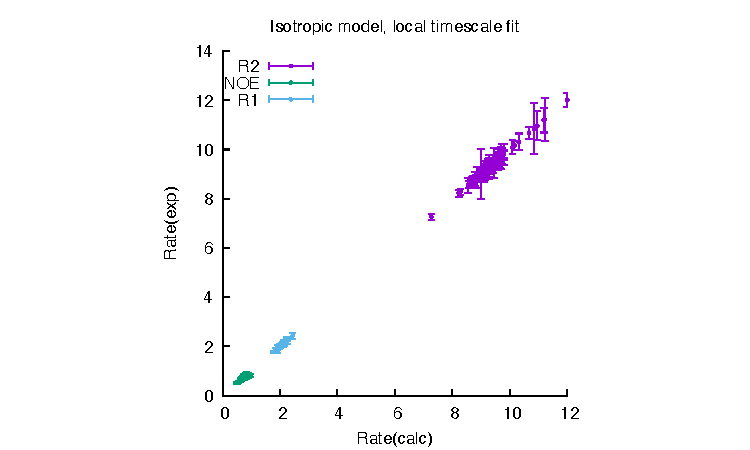
\includegraphics[trim= 3.000000cm 0.000000cm 3.000000cm 0.000000cm ,width=0.202020\textwidth]{bmr11080/LocalTc.600.0.fig2.pdf}
\noindent 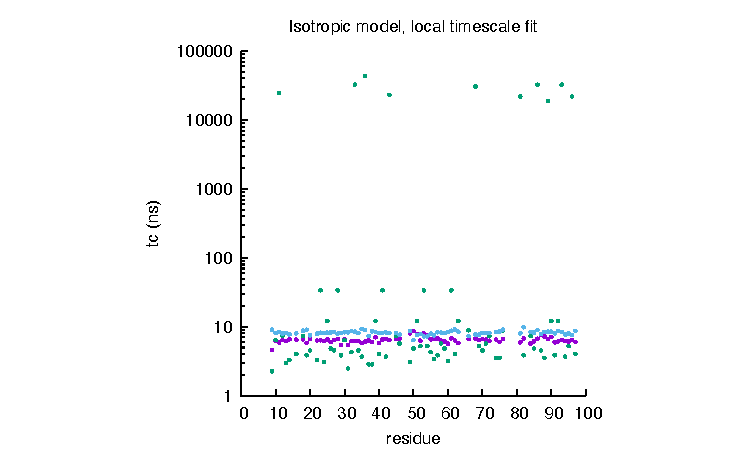
\includegraphics[trim= 3.000000cm 0.000000cm 3.000000cm 0.000000cm ,width=0.202020\textwidth]{bmr11080/LocalTc.600.0.fig3.pdf}
\noindent 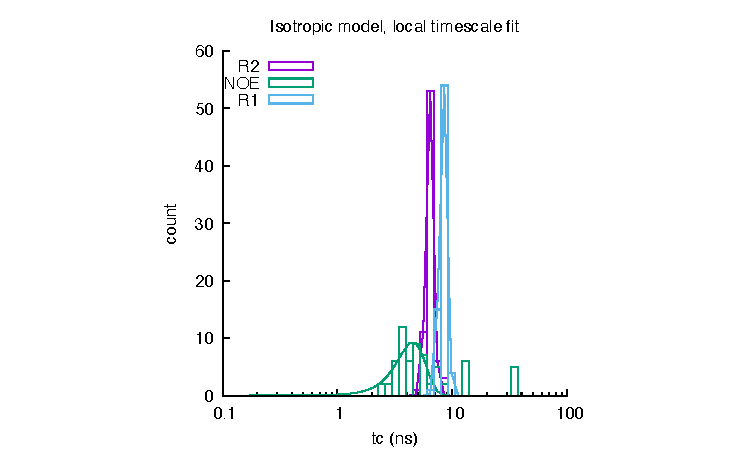
\includegraphics[trim= 3.000000cm 0.000000cm 3.000000cm 0.000000cm ,width=0.202020\textwidth]{bmr11080/LocalTc.600.0.fig4.pdf}
\noindent \subsection{bmr5079: cytochrome c552}

\begin{tabular}{ll}
\textbf{Fields:} &  500.0,600.0 MHz\\
\textbf{DataPts:} &  522\\
 \textbf{T:} & 298 K\\
\textbf{Mw:} & 10.54 kDa\\
\textbf{Residues: } &   100\\
\end{tabular}

\begin{small}
\noindent \begin{tabular}{l|rlrl|rlrl}
& \multicolumn{4}{c}{500.0 MHz}& \multicolumn{4}{c}{600.0 MHz}\\
&  \multicolumn{2}{c}{rate} & \multicolumn{2}{c}{$\tau_c$ (ns)}   &  \multicolumn{2}{c}{rate} & \multicolumn{2}{c}{$\tau_c$ (ns)}   \\
\hline$R_2$  (s$^{-1}$)  &  8.481 & $\pm$ 0.554   &  5.50 & $\pm$ 0.43 &  8.575 & $\pm$ 0.584   &  5.46 & $\pm$ 0.51 \\
NOE  &  0.871 & $\pm$ 0.064   &  5.22 & $\pm$ 0.72 &  0.972 & $\pm$ 0.080   &  5.60 & $\pm$ 0.85 \\
$R_1$ (s$^{-1}$)  &  2.124 & $\pm$ 0.128   &  7.95 & $\pm$ 0.50 &  1.767 & $\pm$ 0.090   &  7.46 & $\pm$ 0.56 \\
$\sigma_{zz}$  (s$^{-1}$)  &  0.051 & $\pm$ 0.005   & & &  0.036 & $\pm$ 0.003   & & \\
$\frac{R_1}{R_2}$  &  0.245 & $\pm$ 0.007   & & &  0.182 & $\pm$ 0.007   & & \\
\end{tabular}
\end{small}


\noindent 
\includegraphics[trim= 3.000000cm 0.000000cm 3.000000cm 0.000000cm ,width=0.202020\textwidth]{bmr5079/LocalTc.800.066.fig0.pdf}
\noindent 
\includegraphics[trim= 3.000000cm 0.000000cm 3.000000cm 0.000000cm ,width=0.202020\textwidth]{bmr5079/LocalTc.800.066.fig1.pdf}
\noindent 
\includegraphics[trim= 3.000000cm 0.000000cm 3.000000cm 0.000000cm ,width=0.202020\textwidth]{bmr5079/LocalTc.800.066.fig2.pdf}
\noindent 
\includegraphics[trim= 3.000000cm 0.000000cm 3.000000cm 0.000000cm ,width=0.202020\textwidth]{bmr5079/LocalTc.800.066.fig3.pdf}
\noindent 
\includegraphics[trim= 3.000000cm 0.000000cm 3.000000cm 0.000000cm ,width=0.202020\textwidth]{bmr5079/LocalTc.800.066.fig4.pdf}
\noindent 
\includegraphics[trim= 3.000000cm 0.000000cm 3.000000cm 0.000000cm ,width=0.202020\textwidth]{bmr5079/LocalTc.500.0.fig0.pdf}
\noindent 
\includegraphics[trim= 3.000000cm 0.000000cm 3.000000cm 0.000000cm ,width=0.202020\textwidth]{bmr5079/LocalTc.500.0.fig1.pdf}
\noindent 
\includegraphics[trim= 3.000000cm 0.000000cm 3.000000cm 0.000000cm ,width=0.202020\textwidth]{bmr5079/LocalTc.500.0.fig2.pdf}
\noindent 
\includegraphics[trim= 3.000000cm 0.000000cm 3.000000cm 0.000000cm ,width=0.202020\textwidth]{bmr5079/LocalTc.500.0.fig3.pdf}
\noindent 
\includegraphics[trim= 3.000000cm 0.000000cm 3.000000cm 0.000000cm ,width=0.202020\textwidth]{bmr5079/LocalTc.500.0.fig4.pdf}
\noindent \subsection{bmr5080: cytochrome c552}

\begin{tabular}{ll}
\textbf{Fields:} &  500.0,600.0 MHz\\
\textbf{DataPts:} &  528\\
 \textbf{T:} & 298 K\\
\textbf{Mw:} & 10.54 kDa\\
\textbf{Residues: } &   100\\
\end{tabular}

\begin{small}
\noindent \begin{tabular}{l|rlrl|rlrl}
& \multicolumn{4}{c}{500.0 MHz}& \multicolumn{4}{c}{600.0 MHz}\\
&  \multicolumn{2}{c}{rate} & \multicolumn{2}{c}{$\tau_c$ (ns)}   &  \multicolumn{2}{c}{rate} & \multicolumn{2}{c}{$\tau_c$ (ns)}   \\
\hline$R_2$  (s$^{-1}$)  &  10.163 & $\pm$ 0.702   &  7.04 & $\pm$ 0.59 &  10.033 & $\pm$ 0.552   &  6.49 & $\pm$ 0.56 \\
NOE  &  1.010 & $\pm$ 0.101   &  4.71 & $\pm$ 0.52 &  0.973 & $\pm$ 0.087   &  5.13 & $\pm$ 1.13 \\
$R_1$ (s$^{-1}$)  &  1.950 & $\pm$ 0.086   &  9.10 & $\pm$ 0.32 &  1.649 & $\pm$ 0.069   &  7.93 & $\pm$ 0.45 \\
$\sigma_{zz}$  (s$^{-1}$)  &  0.050 & $\pm$ 0.004   & & &  0.035 & $\pm$ 0.003   & & \\
$\frac{R_1}{R_2}$  &  0.196 & $\pm$ 0.006   & & &  0.164 & $\pm$ 0.004   & & \\
\end{tabular}
\end{small}


\noindent 
\includegraphics[trim= 3.000000cm 0.000000cm 3.000000cm 0.000000cm ,width=0.202020\textwidth]{bmr5080/LocalTc.600.0.fig0.pdf}
\noindent 
\includegraphics[trim= 3.000000cm 0.000000cm 3.000000cm 0.000000cm ,width=0.202020\textwidth]{bmr5080/LocalTc.600.0.fig1.pdf}
\noindent 
\includegraphics[trim= 3.000000cm 0.000000cm 3.000000cm 0.000000cm ,width=0.202020\textwidth]{bmr5080/LocalTc.600.0.fig2.pdf}
\noindent 
\includegraphics[trim= 3.000000cm 0.000000cm 3.000000cm 0.000000cm ,width=0.202020\textwidth]{bmr5080/LocalTc.600.0.fig3.pdf}
\noindent 
\includegraphics[trim= 3.000000cm 0.000000cm 3.000000cm 0.000000cm ,width=0.202020\textwidth]{bmr5080/LocalTc.600.0.fig4.pdf}
\noindent 
\includegraphics[trim= 3.000000cm 0.000000cm 3.000000cm 0.000000cm ,width=0.202020\textwidth]{bmr5080/LocalTc.500.0.fig0.pdf}
\noindent 
\includegraphics[trim= 3.000000cm 0.000000cm 3.000000cm 0.000000cm ,width=0.202020\textwidth]{bmr5080/LocalTc.500.0.fig1.pdf}
\noindent 
\includegraphics[trim= 3.000000cm 0.000000cm 3.000000cm 0.000000cm ,width=0.202020\textwidth]{bmr5080/LocalTc.500.0.fig2.pdf}
\noindent 
\includegraphics[trim= 3.000000cm 0.000000cm 3.000000cm 0.000000cm ,width=0.202020\textwidth]{bmr5080/LocalTc.500.0.fig3.pdf}
\noindent 
\includegraphics[trim= 3.000000cm 0.000000cm 3.000000cm 0.000000cm ,width=0.202020\textwidth]{bmr5080/LocalTc.500.0.fig4.pdf}
\noindent \subsection{bmr15437: S836 monomer}

\begin{tabular}{ll}
\textbf{Fields:} &  500.0,600.0 MHz\\
\textbf{DataPts:} &  594\\
 \textbf{T:} & 298 K\\
\textbf{Mw:} & 11.93 kDa\\
\textbf{Residues: } &   102\\
\end{tabular}

\begin{small}
\noindent \begin{tabular}{l|rlrl|rlrl}
& \multicolumn{4}{c}{500.0 MHz}& \multicolumn{4}{c}{600.0 MHz}\\
&  \multicolumn{2}{c}{rate} & \multicolumn{2}{c}{$\tau_c$ (ns)}   &  \multicolumn{2}{c}{rate} & \multicolumn{2}{c}{$\tau_c$ (ns)}   \\
\hline$R_2$  (s$^{-1}$)  &  10.104 & $\pm$ 0.657   &  7.23 & $\pm$ 0.79 &  11.950 & $\pm$ 1.260   &  8.26 & $\pm$ 1.04 \\
NOE  &  0.826 & $\pm$ 0.097   &  4.58 & $\pm$ 1.84 &  0.772 & $\pm$ 0.089   &  3.22 & $\pm$ 1.00 \\
$R_1$ (s$^{-1}$)  &  2.092 & $\pm$ 0.051   &  8.15 & $\pm$ 0.66 &  1.659 & $\pm$ 0.030   &  7.80 & $\pm$ 0.51 \\
$\sigma_{zz}$  (s$^{-1}$)  &  0.058 & $\pm$ 0.028   & & &  0.045 & $\pm$ 0.018   & & \\
$\frac{R_1}{R_2}$  &  0.220 & $\pm$ 0.067   & & &  0.109 & $\pm$ 0.035   & & \\
\end{tabular}
\end{small}


\noindent 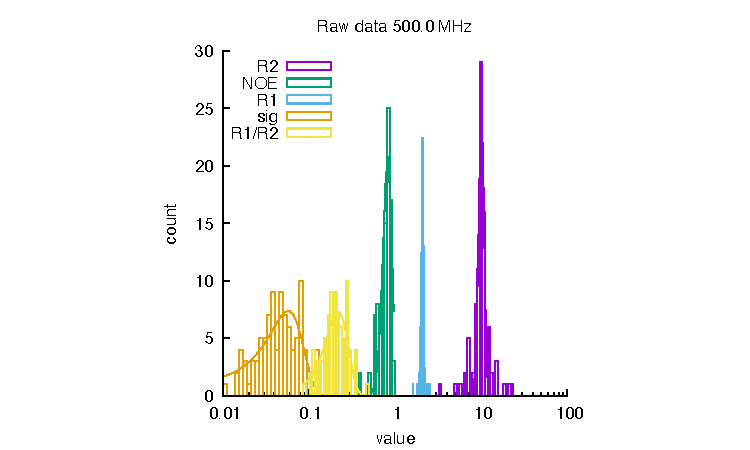
\includegraphics[trim= 3.000000cm 0.000000cm 3.000000cm 0.000000cm ,width=0.202020\textwidth]{bmr15437/LocalTc.600.12282197.fig0.pdf}
\noindent 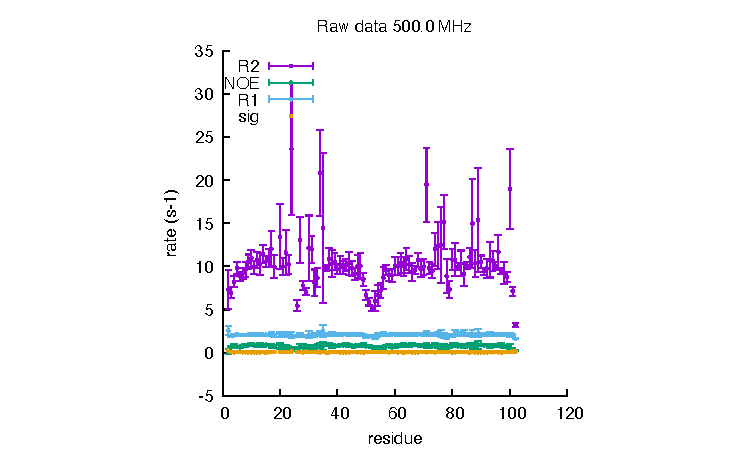
\includegraphics[trim= 3.000000cm 0.000000cm 3.000000cm 0.000000cm ,width=0.202020\textwidth]{bmr15437/LocalTc.600.12282197.fig1.pdf}
\noindent 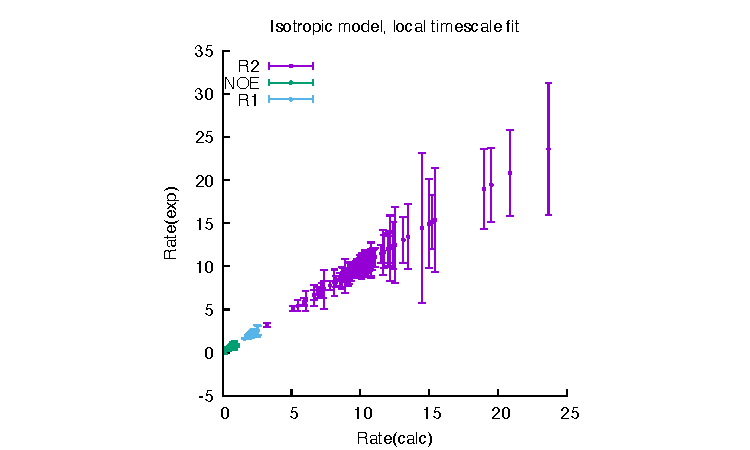
\includegraphics[trim= 3.000000cm 0.000000cm 3.000000cm 0.000000cm ,width=0.202020\textwidth]{bmr15437/LocalTc.600.12282197.fig2.pdf}
\noindent 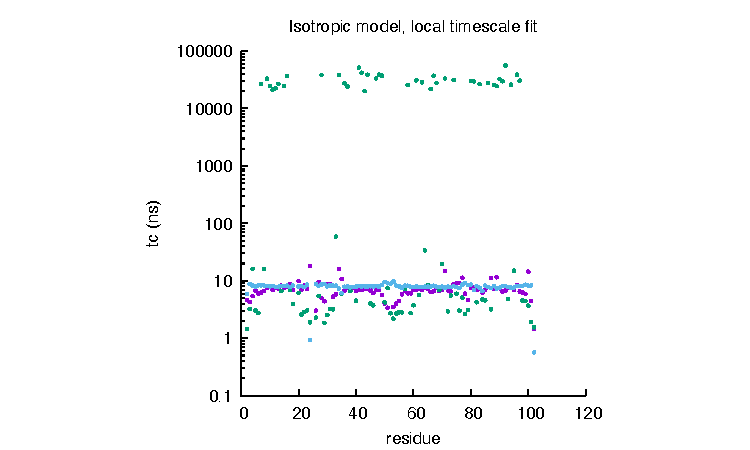
\includegraphics[trim= 3.000000cm 0.000000cm 3.000000cm 0.000000cm ,width=0.202020\textwidth]{bmr15437/LocalTc.600.12282197.fig3.pdf}
\noindent 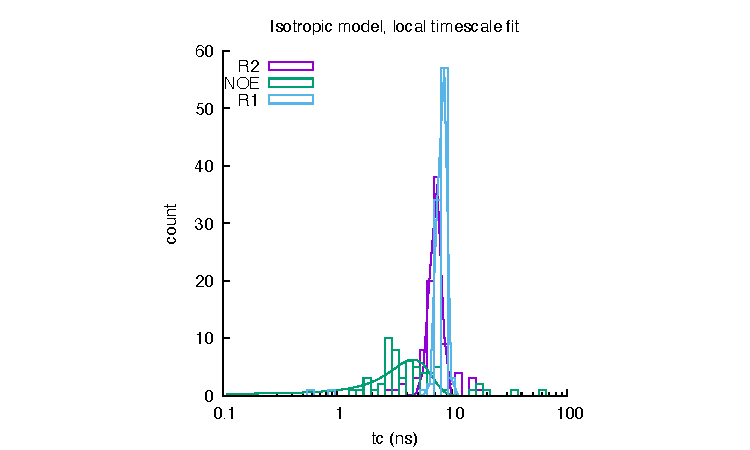
\includegraphics[trim= 3.000000cm 0.000000cm 3.000000cm 0.000000cm ,width=0.202020\textwidth]{bmr15437/LocalTc.600.12282197.fig4.pdf}
\noindent 
\includegraphics[trim= 3.000000cm 0.000000cm 3.000000cm 0.000000cm ,width=0.202020\textwidth]{bmr15437/LocalTc.500.0.fig0.pdf}
\noindent 
\includegraphics[trim= 3.000000cm 0.000000cm 3.000000cm 0.000000cm ,width=0.202020\textwidth]{bmr15437/LocalTc.500.0.fig1.pdf}
\noindent 
\includegraphics[trim= 3.000000cm 0.000000cm 3.000000cm 0.000000cm ,width=0.202020\textwidth]{bmr15437/LocalTc.500.0.fig2.pdf}
\noindent 
\includegraphics[trim= 3.000000cm 0.000000cm 3.000000cm 0.000000cm ,width=0.202020\textwidth]{bmr15437/LocalTc.500.0.fig3.pdf}
\noindent 
\includegraphics[trim= 3.000000cm 0.000000cm 3.000000cm 0.000000cm ,width=0.202020\textwidth]{bmr15437/LocalTc.500.0.fig4.pdf}
\noindent \subsection{bmr5687: protein S-824}

\begin{tabular}{ll}
\textbf{Fields:} &  500.0,600.0 MHz\\
\textbf{DataPts:} &  606\\
 \textbf{T:} & 298 K\\
\textbf{Mw:} & 11.93 kDa\\
\textbf{Residues: } &   102\\
\end{tabular}

\begin{small}
\noindent \begin{tabular}{l|rlrl|rlrl}
& \multicolumn{4}{c}{500.0 MHz}& \multicolumn{4}{c}{600.0 MHz}\\
&  \multicolumn{2}{c}{rate} & \multicolumn{2}{c}{$\tau_c$ (ns)}   &  \multicolumn{2}{c}{rate} & \multicolumn{2}{c}{$\tau_c$ (ns)}   \\
\hline$R_2$  (s$^{-1}$)  &  9.376 & $\pm$ 0.461   &  6.44 & $\pm$ 0.51 &  11.127 & $\pm$ 0.579   &  7.51 & $\pm$ 0.62 \\
NOE  &  0.803 & $\pm$ 0.091   &  4.90 & $\pm$ 1.83 &  0.784 & $\pm$ 0.096   &  3.24 & $\pm$ 0.85 \\
$R_1$ (s$^{-1}$)  &  2.096 & $\pm$ 0.035   &  8.16 & $\pm$ 0.64 &  1.649 & $\pm$ 0.042   &  7.83 & $\pm$ 0.52 \\
$\sigma_{zz}$  (s$^{-1}$)  &  0.053 & $\pm$ 0.019   & & &  0.043 & $\pm$ 0.015   & & \\
$\frac{R_1}{R_2}$  &  0.280 & $\pm$ 0.055   & & &  0.123 & $\pm$ 0.028   & & \\
\end{tabular}
\end{small}


\noindent 
\includegraphics[trim= 3.000000cm 0.000000cm 3.000000cm 0.000000cm ,width=0.202020\textwidth]{bmr5687/LocalTc.600.0.fig0.pdf}
\noindent 
\includegraphics[trim= 3.000000cm 0.000000cm 3.000000cm 0.000000cm ,width=0.202020\textwidth]{bmr5687/LocalTc.600.0.fig1.pdf}
\noindent 
\includegraphics[trim= 3.000000cm 0.000000cm 3.000000cm 0.000000cm ,width=0.202020\textwidth]{bmr5687/LocalTc.600.0.fig2.pdf}
\noindent 
\includegraphics[trim= 3.000000cm 0.000000cm 3.000000cm 0.000000cm ,width=0.202020\textwidth]{bmr5687/LocalTc.600.0.fig3.pdf}
\noindent 
\includegraphics[trim= 3.000000cm 0.000000cm 3.000000cm 0.000000cm ,width=0.202020\textwidth]{bmr5687/LocalTc.600.0.fig4.pdf}
\noindent 
\includegraphics[trim= 3.000000cm 0.000000cm 3.000000cm 0.000000cm ,width=0.202020\textwidth]{bmr5687/LocalTc.500.0.fig0.pdf}
\noindent 
\includegraphics[trim= 3.000000cm 0.000000cm 3.000000cm 0.000000cm ,width=0.202020\textwidth]{bmr5687/LocalTc.500.0.fig1.pdf}
\noindent 
\includegraphics[trim= 3.000000cm 0.000000cm 3.000000cm 0.000000cm ,width=0.202020\textwidth]{bmr5687/LocalTc.500.0.fig2.pdf}
\noindent 
\includegraphics[trim= 3.000000cm 0.000000cm 3.000000cm 0.000000cm ,width=0.202020\textwidth]{bmr5687/LocalTc.500.0.fig3.pdf}
\noindent 
\includegraphics[trim= 3.000000cm 0.000000cm 3.000000cm 0.000000cm ,width=0.202020\textwidth]{bmr5687/LocalTc.500.0.fig4.pdf}
\noindent \subsection{bmr18758: First Catalytic Cysteine Half-domain}

\begin{tabular}{ll}
\textbf{Fields:} &  400.0 MHz\\
\textbf{DataPts:} &  291\\
 \textbf{T:} & 298 K\\
\textbf{Mw:} & 12.19 kDa\\
\textbf{Residues: } &   112\\
\end{tabular}

\begin{small}
\noindent \begin{tabular}{l|rlrl}
& \multicolumn{4}{c}{400.0 MHz}\\
&  \multicolumn{2}{c}{rate} & \multicolumn{2}{c}{$\tau_c$ (ns)}   \\
\hline$R_2$  (s$^{-1}$)  &  11.356 & $\pm$ 0.929   &  8.38 & $\pm$ 0.99 \\
NOE  &  0.695 & $\pm$ 0.075   &  4.85 & $\pm$ 1.08 \\
$R_1$ (s$^{-1}$)  &  2.209 & $\pm$ 0.139   &  11.62 & $\pm$ 0.94 \\
$\sigma_{zz}$  (s$^{-1}$)  &  0.072 & $\pm$ 0.012   & & \\
$\frac{R_1}{R_2}$  &  0.130 & $\pm$ 0.016   & & \\
\end{tabular}
\end{small}


\noindent 
\includegraphics[trim= 3.000000cm 0.000000cm 3.000000cm 0.000000cm ,width=0.202020\textwidth]{bmr18758/LocalTc.600.0.fig0.pdf}
\noindent 
\includegraphics[trim= 3.000000cm 0.000000cm 3.000000cm 0.000000cm ,width=0.202020\textwidth]{bmr18758/LocalTc.600.0.fig1.pdf}
\noindent 
\includegraphics[trim= 3.000000cm 0.000000cm 3.000000cm 0.000000cm ,width=0.202020\textwidth]{bmr18758/LocalTc.600.0.fig2.pdf}
\noindent 
\includegraphics[trim= 3.000000cm 0.000000cm 3.000000cm 0.000000cm ,width=0.202020\textwidth]{bmr18758/LocalTc.600.0.fig3.pdf}
\noindent 
\includegraphics[trim= 3.000000cm 0.000000cm 3.000000cm 0.000000cm ,width=0.202020\textwidth]{bmr18758/LocalTc.600.0.fig4.pdf}
\noindent \subsection{bmr17010: Tryptophan apo-repressor}

\begin{tabular}{ll}
\textbf{Fields:} &  600.0 MHz\\
\textbf{DataPts:} &  216\\
 \textbf{T:} & 318 K\\
\textbf{Mw:} & 12.36 kDa\\
\textbf{Residues: } &   108\\
\end{tabular}

\begin{small}
\noindent \begin{tabular}{l|rlrl}
& \multicolumn{4}{c}{600.0 MHz}\\
&  \multicolumn{2}{c}{rate} & \multicolumn{2}{c}{$\tau_c$ (ns)}   \\
\hline$R_2$  (s$^{-1}$)  &  13.106 & $\pm$ 0.776   &  8.95 & $\pm$ 0.69 \\
NOE  &  2.824 & $\pm$ 0.467   &  4.63 & $\pm$ 1.76 \\
$R_1$ (s$^{-1}$)  &  1.217 & $\pm$ 0.070   &  11.41 & $\pm$ 0.89 \\
$\sigma_{zz}$  (s$^{-1}$)  &  0.026 & $\pm$ 0.004   & & \\
$\frac{R_1}{R_2}$  &  0.076 & $\pm$ 0.010   & & \\
\end{tabular}
\end{small}


\noindent 
\includegraphics[trim= 3.000000cm 0.000000cm 3.000000cm 0.000000cm ,width=0.202020\textwidth]{bmr17010/LocalTc.600.0.fig0.pdf}
\noindent 
\includegraphics[trim= 3.000000cm 0.000000cm 3.000000cm 0.000000cm ,width=0.202020\textwidth]{bmr17010/LocalTc.600.0.fig1.pdf}
\noindent 
\includegraphics[trim= 3.000000cm 0.000000cm 3.000000cm 0.000000cm ,width=0.202020\textwidth]{bmr17010/LocalTc.600.0.fig2.pdf}
\noindent 
\includegraphics[trim= 3.000000cm 0.000000cm 3.000000cm 0.000000cm ,width=0.202020\textwidth]{bmr17010/LocalTc.600.0.fig3.pdf}
\noindent 
\includegraphics[trim= 3.000000cm 0.000000cm 3.000000cm 0.000000cm ,width=0.202020\textwidth]{bmr17010/LocalTc.600.0.fig4.pdf}
\noindent \subsection{bmr17013: Tryptophan apo-repressor}

\begin{tabular}{ll}
\textbf{Fields:} &  600.0 MHz\\
\textbf{DataPts:} &  240\\
 \textbf{T:} & 318 K\\
\textbf{Mw:} & 12.38 kDa\\
\textbf{Residues: } &   108\\
\end{tabular}

\begin{small}
\noindent \begin{tabular}{l|rlrl}
& \multicolumn{4}{c}{600.0 MHz}\\
&  \multicolumn{2}{c}{rate} & \multicolumn{2}{c}{$\tau_c$ (ns)}   \\
\hline$R_2$  (s$^{-1}$)  &  13.063 & $\pm$ 1.003   &  8.99 & $\pm$ 0.75 \\
NOE  &  0.855 & $\pm$ 0.104   &  4.50 & $\pm$ 1.60 \\
$R_1$ (s$^{-1}$)  &  1.198 & $\pm$ 0.081   &  11.66 & $\pm$ 1.01 \\
$\sigma_{zz}$  (s$^{-1}$)  &  0.028 & $\pm$ 0.007   & & \\
$\frac{R_1}{R_2}$  &  0.106 & $\pm$ 0.023   & & \\
\end{tabular}
\end{small}


\noindent 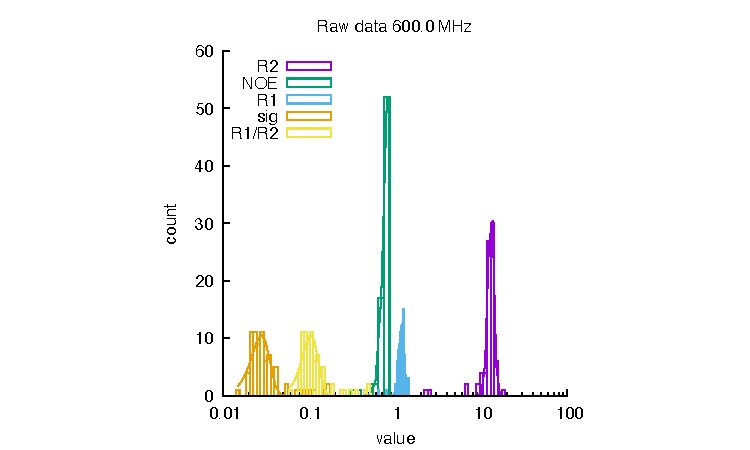
\includegraphics[trim= 3.000000cm 0.000000cm 3.000000cm 0.000000cm ,width=0.202020\textwidth]{bmr17013/LocalTc.500.fig0.pdf}
\noindent 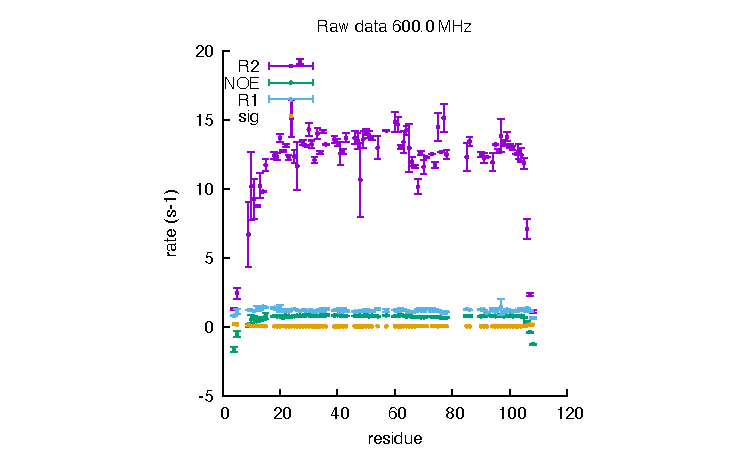
\includegraphics[trim= 3.000000cm 0.000000cm 3.000000cm 0.000000cm ,width=0.202020\textwidth]{bmr17013/LocalTc.500.fig1.pdf}
\noindent 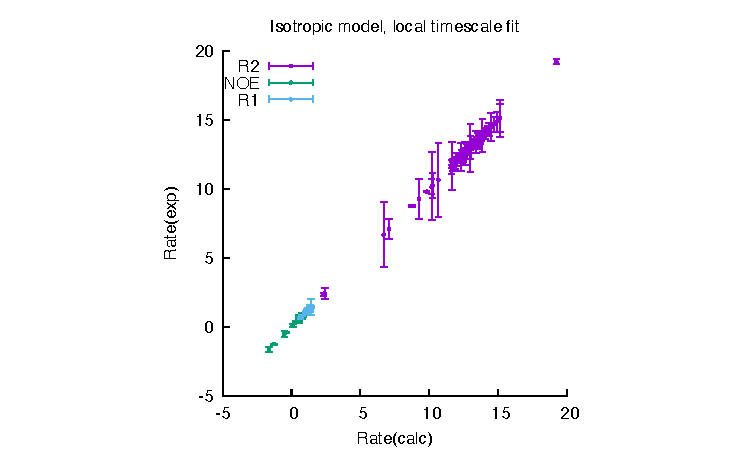
\includegraphics[trim= 3.000000cm 0.000000cm 3.000000cm 0.000000cm ,width=0.202020\textwidth]{bmr17013/LocalTc.500.fig2.pdf}
\noindent 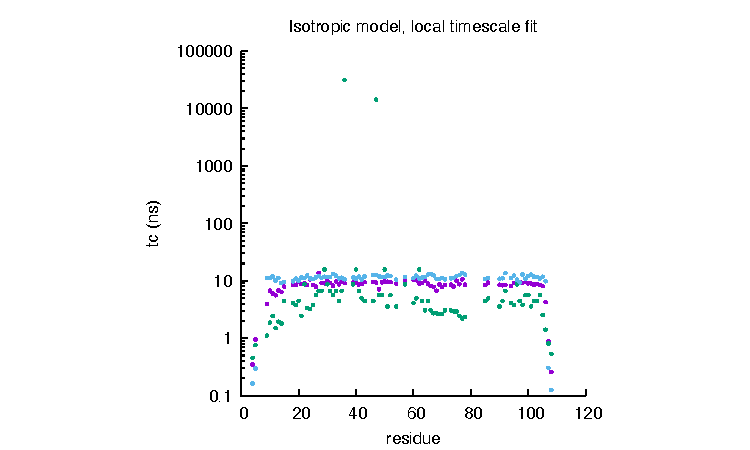
\includegraphics[trim= 3.000000cm 0.000000cm 3.000000cm 0.000000cm ,width=0.202020\textwidth]{bmr17013/LocalTc.500.fig3.pdf}
\noindent 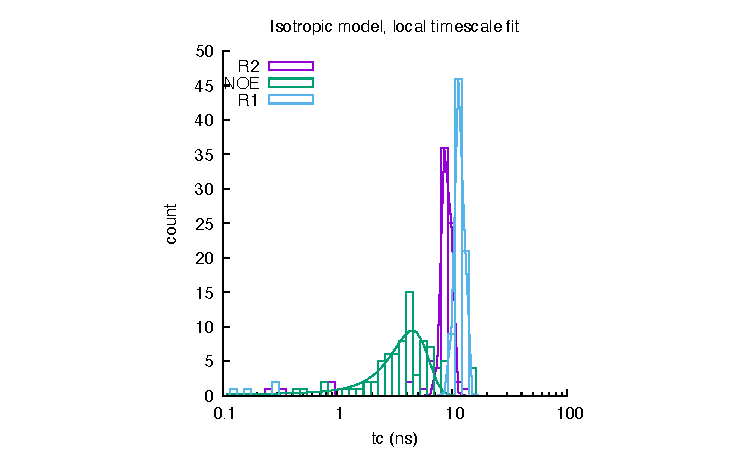
\includegraphics[trim= 3.000000cm 0.000000cm 3.000000cm 0.000000cm ,width=0.202020\textwidth]{bmr17013/LocalTc.500.fig4.pdf}
\noindent \subsection{bmr17012: Tryptophan apo-repressor}

\begin{tabular}{ll}
\textbf{Fields:} &  600.0 MHz\\
\textbf{DataPts:} &  276\\
 \textbf{T:} & 318 K\\
\textbf{Mw:} & 12.39 kDa\\
\textbf{Residues: } &   108\\
\end{tabular}

\begin{small}
\noindent \begin{tabular}{l|rlrl}
& \multicolumn{4}{c}{600.0 MHz}\\
&  \multicolumn{2}{c}{rate} & \multicolumn{2}{c}{$\tau_c$ (ns)}   \\
\hline$R_2$  (s$^{-1}$)  &  13.454 & $\pm$ 1.064   &  9.28 & $\pm$ 1.01 \\
NOE  &  1.736 & $\pm$ 0.396   &  4.03 & $\pm$ 1.58 \\
$R_1$ (s$^{-1}$)  &  1.223 & $\pm$ 0.079   &  11.27 & $\pm$ 0.91 \\
$\sigma_{zz}$  (s$^{-1}$)  &  0.026 & $\pm$ 0.004   & & \\
$\frac{R_1}{R_2}$  &  0.102 & $\pm$ 0.012   & & \\
\end{tabular}
\end{small}


\noindent 
\includegraphics[trim= 3.000000cm 0.000000cm 3.000000cm 0.000000cm ,width=0.202020\textwidth]{bmr17012/LocalTc.600.0.fig0.pdf}
\noindent 
\includegraphics[trim= 3.000000cm 0.000000cm 3.000000cm 0.000000cm ,width=0.202020\textwidth]{bmr17012/LocalTc.600.0.fig1.pdf}
\noindent 
\includegraphics[trim= 3.000000cm 0.000000cm 3.000000cm 0.000000cm ,width=0.202020\textwidth]{bmr17012/LocalTc.600.0.fig2.pdf}
\noindent 
\includegraphics[trim= 3.000000cm 0.000000cm 3.000000cm 0.000000cm ,width=0.202020\textwidth]{bmr17012/LocalTc.600.0.fig3.pdf}
\noindent 
\includegraphics[trim= 3.000000cm 0.000000cm 3.000000cm 0.000000cm ,width=0.202020\textwidth]{bmr17012/LocalTc.600.0.fig4.pdf}
\noindent \subsection{bmr17041: holoTrpR dimer}

\begin{tabular}{ll}
\textbf{Fields:} &  600.0 MHz\\
\textbf{DataPts:} &  228\\
 \textbf{T:} & 318 K\\
\textbf{Mw:} & 13.05 kDa\\
\textbf{Residues: } &   113\\
\end{tabular}

\begin{small}
\noindent \begin{tabular}{l|rlrl}
& \multicolumn{4}{c}{600.0 MHz}\\
&  \multicolumn{2}{c}{rate} & \multicolumn{2}{c}{$\tau_c$ (ns)}   \\
\hline$R_2$  (s$^{-1}$)  &  13.383 & $\pm$ 0.900   &  9.14 & $\pm$ 0.78 \\
NOE  &  2.290 & $\pm$ 0.366   &  4.60 & $\pm$ 1.52 \\
$R_1$ (s$^{-1}$)  &  1.231 & $\pm$ 0.075   &  11.11 & $\pm$ 0.88 \\
$\sigma_{zz}$  (s$^{-1}$)  &  0.027 & $\pm$ 0.005   & & \\
$\frac{R_1}{R_2}$  &  0.112 & $\pm$ 0.019   & & \\
\end{tabular}
\end{small}


\noindent 
\includegraphics[trim= 3.000000cm 0.000000cm 3.000000cm 0.000000cm ,width=0.202020\textwidth]{bmr17041/LocalTc.600.0.fig0.pdf}
\noindent 
\includegraphics[trim= 3.000000cm 0.000000cm 3.000000cm 0.000000cm ,width=0.202020\textwidth]{bmr17041/LocalTc.600.0.fig1.pdf}
\noindent 
\includegraphics[trim= 3.000000cm 0.000000cm 3.000000cm 0.000000cm ,width=0.202020\textwidth]{bmr17041/LocalTc.600.0.fig2.pdf}
\noindent 
\includegraphics[trim= 3.000000cm 0.000000cm 3.000000cm 0.000000cm ,width=0.202020\textwidth]{bmr17041/LocalTc.600.0.fig3.pdf}
\noindent 
\includegraphics[trim= 3.000000cm 0.000000cm 3.000000cm 0.000000cm ,width=0.202020\textwidth]{bmr17041/LocalTc.600.0.fig4.pdf}
\noindent \subsection{bmr17047: holoTrpR dimer A77V variant}

\begin{tabular}{ll}
\textbf{Fields:} &  600.0 MHz\\
\textbf{DataPts:} &  246\\
 \textbf{T:} & 318 K\\
\textbf{Mw:} & 13.07 kDa\\
\textbf{Residues: } &   113\\
\end{tabular}

\begin{small}
\noindent \begin{tabular}{l|rlrl}
& \multicolumn{4}{c}{600.0 MHz}\\
&  \multicolumn{2}{c}{rate} & \multicolumn{2}{c}{$\tau_c$ (ns)}   \\
\hline$R_2$  (s$^{-1}$)  &  13.683 & $\pm$ 0.862   &  9.48 & $\pm$ 0.75 \\
NOE  &  0.799 & $\pm$ 0.093   &  4.12 & $\pm$ 1.56 \\
$R_1$ (s$^{-1}$)  &  1.131 & $\pm$ 0.063   &  12.24 & $\pm$ 1.04 \\
$\sigma_{zz}$  (s$^{-1}$)  &  0.027 & $\pm$ 0.007   & & \\
$\frac{R_1}{R_2}$  &  0.160 & $\pm$ 0.035   & & \\
\end{tabular}
\end{small}


\noindent 
\includegraphics[trim= 3.000000cm 0.000000cm 3.000000cm 0.000000cm ,width=0.202020\textwidth]{bmr17047/LocalTc.500.0.fig0.pdf}
\noindent 
\includegraphics[trim= 3.000000cm 0.000000cm 3.000000cm 0.000000cm ,width=0.202020\textwidth]{bmr17047/LocalTc.500.0.fig1.pdf}
\noindent 
\includegraphics[trim= 3.000000cm 0.000000cm 3.000000cm 0.000000cm ,width=0.202020\textwidth]{bmr17047/LocalTc.500.0.fig2.pdf}
\noindent 
\includegraphics[trim= 3.000000cm 0.000000cm 3.000000cm 0.000000cm ,width=0.202020\textwidth]{bmr17047/LocalTc.500.0.fig3.pdf}
\noindent 
\includegraphics[trim= 3.000000cm 0.000000cm 3.000000cm 0.000000cm ,width=0.202020\textwidth]{bmr17047/LocalTc.500.0.fig4.pdf}
\noindent \subsection{bmr17046: holoTrpR dimer L75F variant}

\begin{tabular}{ll}
\textbf{Fields:} &  600.0 MHz\\
\textbf{DataPts:} &  246\\
 \textbf{T:} & 318 K\\
\textbf{Mw:} & 13.08 kDa\\
\textbf{Residues: } &   113\\
\end{tabular}

\begin{small}
\noindent \begin{tabular}{l|rlrl}
& \multicolumn{4}{c}{600.0 MHz}\\
&  \multicolumn{2}{c}{rate} & \multicolumn{2}{c}{$\tau_c$ (ns)}   \\
\hline$R_2$  (s$^{-1}$)  &  12.956 & $\pm$ 0.956   &  8.85 & $\pm$ 0.81 \\
NOE  &  3.002 & $\pm$ 0.482   &  4.15 & $\pm$ 0.37 \\
$R_1$ (s$^{-1}$)  &  1.262 & $\pm$ 0.099   &  11.02 & $\pm$ 1.09 \\
$\sigma_{zz}$  (s$^{-1}$)  &  0.027 & $\pm$ 0.005   & & \\
$\frac{R_1}{R_2}$  &  0.123 & $\pm$ 0.018   & & \\
\end{tabular}
\end{small}


\noindent 
\includegraphics[trim= 3.000000cm 0.000000cm 3.000000cm 0.000000cm ,width=0.202020\textwidth]{bmr17046/LocalTc.600.0.fig0.pdf}
\noindent 
\includegraphics[trim= 3.000000cm 0.000000cm 3.000000cm 0.000000cm ,width=0.202020\textwidth]{bmr17046/LocalTc.600.0.fig1.pdf}
\noindent 
\includegraphics[trim= 3.000000cm 0.000000cm 3.000000cm 0.000000cm ,width=0.202020\textwidth]{bmr17046/LocalTc.600.0.fig2.pdf}
\noindent 
\includegraphics[trim= 3.000000cm 0.000000cm 3.000000cm 0.000000cm ,width=0.202020\textwidth]{bmr17046/LocalTc.600.0.fig3.pdf}
\noindent 
\includegraphics[trim= 3.000000cm 0.000000cm 3.000000cm 0.000000cm ,width=0.202020\textwidth]{bmr17046/LocalTc.600.0.fig4.pdf}
\noindent \subsection{bmr26506: Rho-GTPase Binding Domain}

\begin{tabular}{ll}
\textbf{Fields:} &  600.0 MHz\\
\textbf{DataPts:} &  291\\
 \textbf{T:} & 298 K\\
\textbf{Mw:} & 13.44 kDa\\
\textbf{Residues: } &   122\\
\end{tabular}

\begin{small}
\noindent \begin{tabular}{l|rlrl}
& \multicolumn{4}{c}{600.0 MHz}\\
&  \multicolumn{2}{c}{rate} & \multicolumn{2}{c}{$\tau_c$ (ns)}   \\
\hline$R_2$  (s$^{-1}$)  &  22.097 & $\pm$ 2.042   &  15.79 & $\pm$ 1.71 \\
NOE  &  4.045 & $\pm$ 0.602   &  2.34 & $\pm$ 1.04 \\
$R_1$ (s$^{-1}$)  &  1.589 & $\pm$ 0.085   &  8.59 & $\pm$ 0.75 \\
$\sigma_{zz}$  (s$^{-1}$)  &  0.023 & $\pm$ 0.007   & & \\
$\frac{R_1}{R_2}$  &  0.111 & $\pm$ 0.023   & & \\
\end{tabular}
\end{small}


\noindent 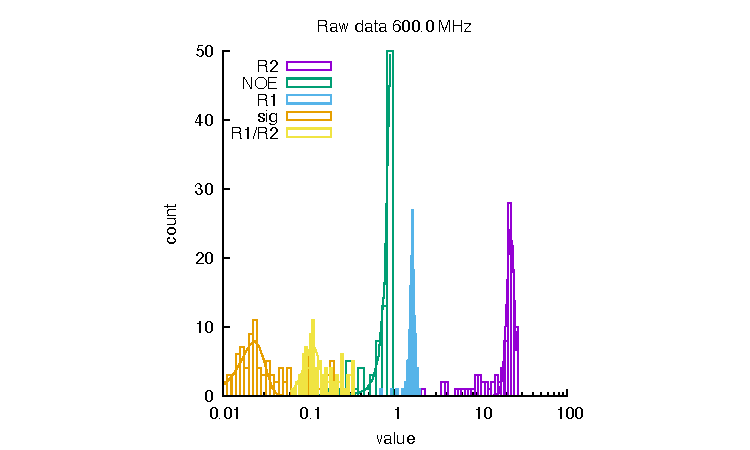
\includegraphics[trim= 3.000000cm 0.000000cm 3.000000cm 0.000000cm ,width=0.202020\textwidth]{bmr26506/LocalTc.950.0.fig0.pdf}
\noindent 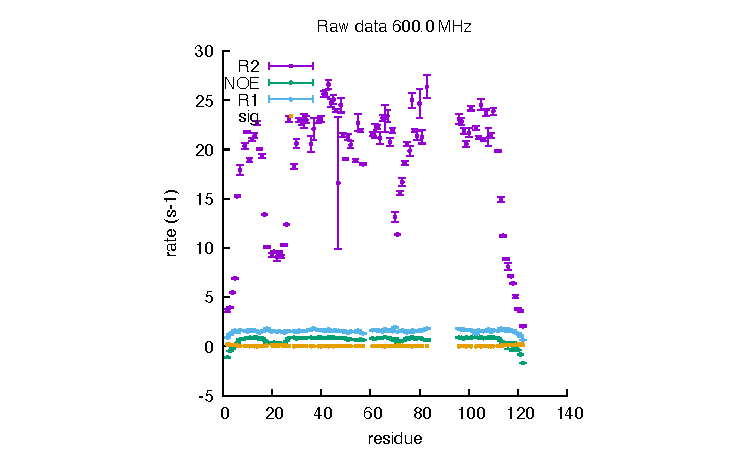
\includegraphics[trim= 3.000000cm 0.000000cm 3.000000cm 0.000000cm ,width=0.202020\textwidth]{bmr26506/LocalTc.950.0.fig1.pdf}
\noindent 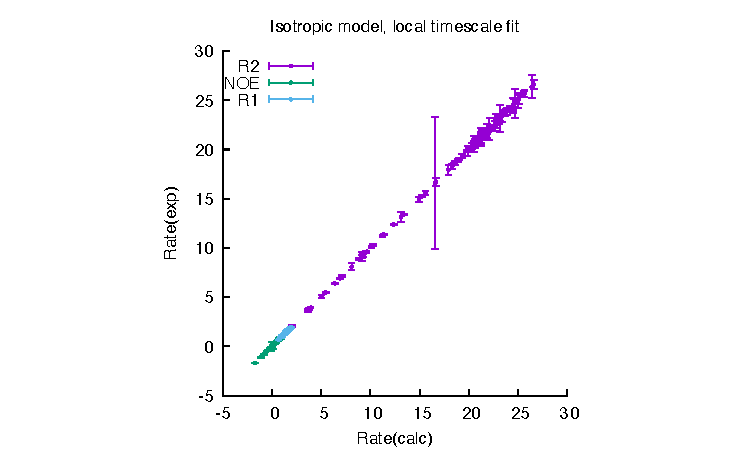
\includegraphics[trim= 3.000000cm 0.000000cm 3.000000cm 0.000000cm ,width=0.202020\textwidth]{bmr26506/LocalTc.950.0.fig2.pdf}
\noindent 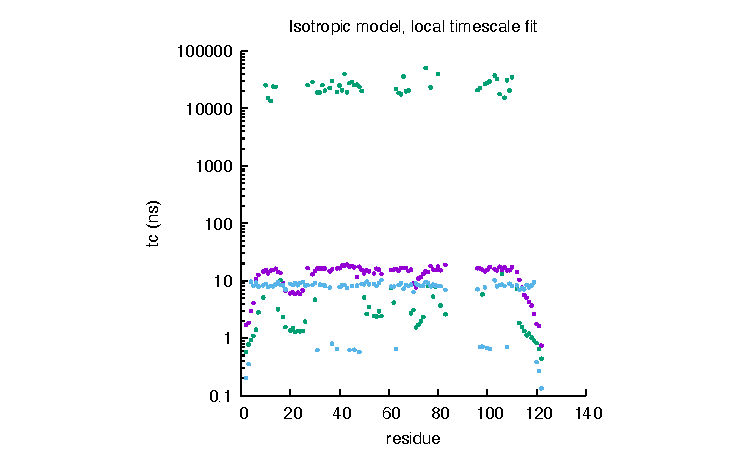
\includegraphics[trim= 3.000000cm 0.000000cm 3.000000cm 0.000000cm ,width=0.202020\textwidth]{bmr26506/LocalTc.950.0.fig3.pdf}
\noindent 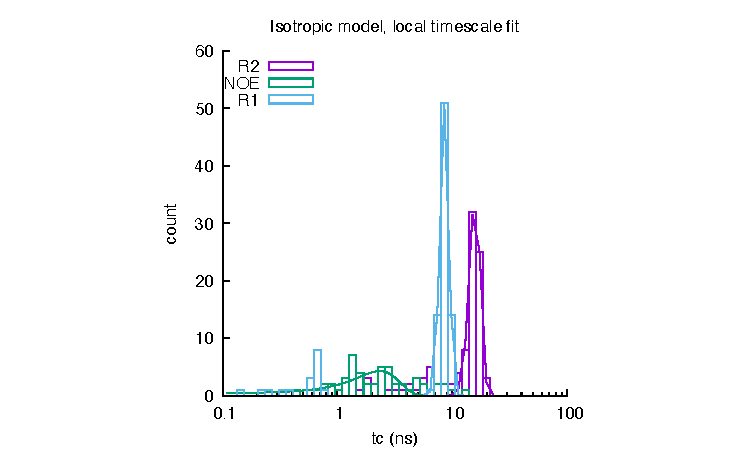
\includegraphics[trim= 3.000000cm 0.000000cm 3.000000cm 0.000000cm ,width=0.202020\textwidth]{bmr26506/LocalTc.950.0.fig4.pdf}
\noindent \subsection{bmr15562: Ymr074cp (1-116) monomer}

\begin{tabular}{ll}
\textbf{Fields:} &  600.1,500.1 MHz\\
\textbf{DataPts:} &  468\\
 \textbf{T:} & 295 K\\
\textbf{Mw:} & 13.77 kDa\\
\textbf{Residues: } &   127\\
\end{tabular}

\begin{small}
\noindent \begin{tabular}{l|rlrl|rlrl}
& \multicolumn{4}{c}{600.13 MHz}& \multicolumn{4}{c}{500.13 MHz}\\
&  \multicolumn{2}{c}{rate} & \multicolumn{2}{c}{$\tau_c$ (ns)}   &  \multicolumn{2}{c}{rate} & \multicolumn{2}{c}{$\tau_c$ (ns)}   \\
\hline$R_2$  (s$^{-1}$)  &  13.112 & $\pm$ 0.761   &  9.07 & $\pm$ 1.00 &  13.044 & $\pm$ 4.457   &  9.72 & $\pm$ 1.41 \\
NOE  &  2.526 & $\pm$ 0.381   &  3.06 & $\pm$ 1.31 &  0.691 & $\pm$ 0.077   &  3.38 & $\pm$ 1.42 \\
$R_1$ (s$^{-1}$)  &  1.418 & $\pm$ 0.067   &  9.39 & $\pm$ 0.87 &  1.658 & $\pm$ 0.083   &  10.72 & $\pm$ 0.87 \\
$\sigma_{zz}$  (s$^{-1}$)  &  0.033 & $\pm$ 0.014   & & &  0.055 & $\pm$ 0.013   & & \\
$\frac{R_1}{R_2}$  &  0.086 & $\pm$ 0.023   & & &  0.115 & $\pm$ 0.017   & & \\
\end{tabular}
\end{small}


\noindent 
\includegraphics[trim= 3.000000cm 0.000000cm 3.000000cm 0.000000cm ,width=0.202020\textwidth]{bmr15562/LocalTc.600.0.fig0.pdf}
\noindent 
\includegraphics[trim= 3.000000cm 0.000000cm 3.000000cm 0.000000cm ,width=0.202020\textwidth]{bmr15562/LocalTc.600.0.fig1.pdf}
\noindent 
\includegraphics[trim= 3.000000cm 0.000000cm 3.000000cm 0.000000cm ,width=0.202020\textwidth]{bmr15562/LocalTc.600.0.fig2.pdf}
\noindent 
\includegraphics[trim= 3.000000cm 0.000000cm 3.000000cm 0.000000cm ,width=0.202020\textwidth]{bmr15562/LocalTc.600.0.fig3.pdf}
\noindent 
\includegraphics[trim= 3.000000cm 0.000000cm 3.000000cm 0.000000cm ,width=0.202020\textwidth]{bmr15562/LocalTc.600.0.fig4.pdf}
\noindent 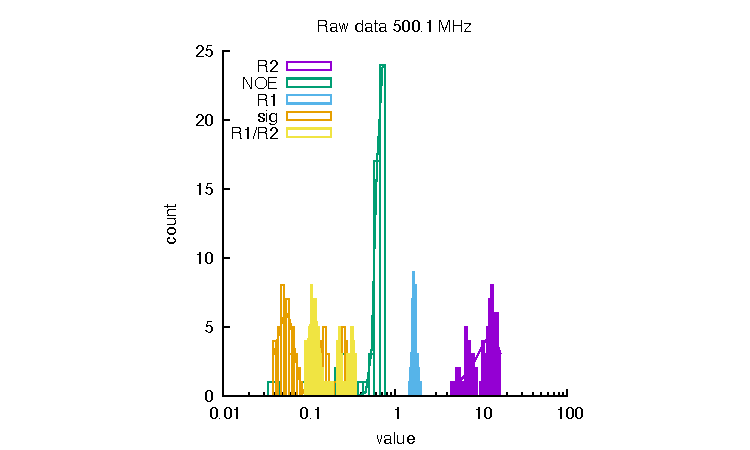
\includegraphics[trim= 3.000000cm 0.000000cm 3.000000cm 0.000000cm ,width=0.202020\textwidth]{bmr15562/LocalTc.600.13.fig0.pdf}
\noindent 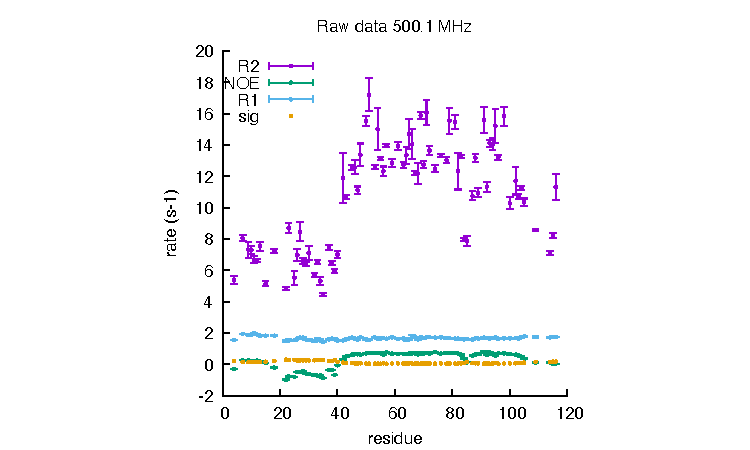
\includegraphics[trim= 3.000000cm 0.000000cm 3.000000cm 0.000000cm ,width=0.202020\textwidth]{bmr15562/LocalTc.600.13.fig1.pdf}
\noindent 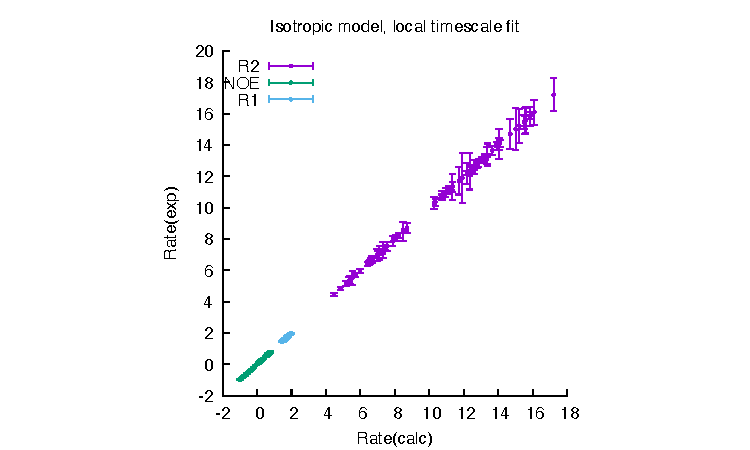
\includegraphics[trim= 3.000000cm 0.000000cm 3.000000cm 0.000000cm ,width=0.202020\textwidth]{bmr15562/LocalTc.600.13.fig2.pdf}
\noindent 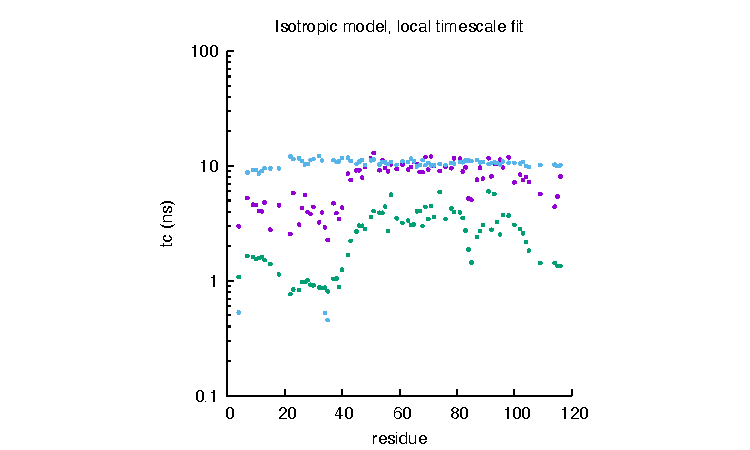
\includegraphics[trim= 3.000000cm 0.000000cm 3.000000cm 0.000000cm ,width=0.202020\textwidth]{bmr15562/LocalTc.600.13.fig3.pdf}
\noindent 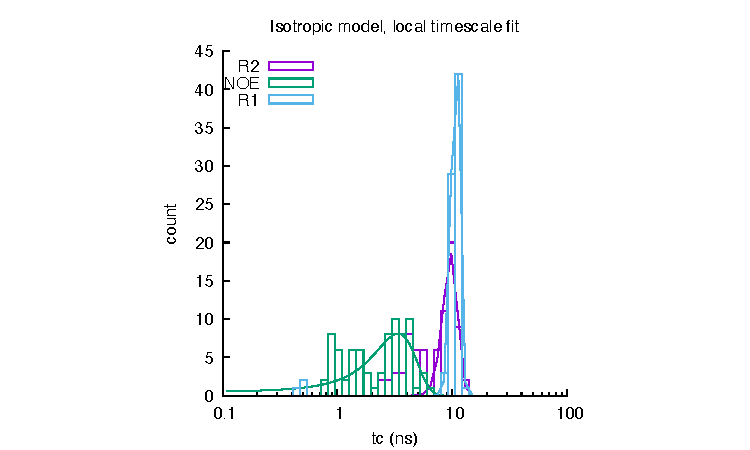
\includegraphics[trim= 3.000000cm 0.000000cm 3.000000cm 0.000000cm ,width=0.202020\textwidth]{bmr15562/LocalTc.600.13.fig4.pdf}
\noindent \subsection{bmr51417: apo Bromodomain 2 (BD2) of BRD4}

\begin{tabular}{ll}
\textbf{Fields:} &  600.0,800.0 MHz\\
\textbf{DataPts:} &  540\\
 \textbf{T:} & 303 K\\
\textbf{Mw:} & 13.92 kDa\\
\textbf{Residues: } &   120\\
\end{tabular}

\begin{small}
\noindent \begin{tabular}{l|rlrl|rlrl}
& \multicolumn{4}{c}{600.0 MHz}& \multicolumn{4}{c}{800.0 MHz}\\
&  \multicolumn{2}{c}{rate} & \multicolumn{2}{c}{$\tau_c$ (ns)}   &  \multicolumn{2}{c}{rate} & \multicolumn{2}{c}{$\tau_c$ (ns)}   \\
\hline$R_2$  (s$^{-1}$)  &  14.394 & $\pm$ 1.224   &  10.02 & $\pm$ 1.02 &  17.847 & $\pm$ 1.358   &  10.81 & $\pm$ 1.16 \\
NOE  &  1.002 & $\pm$ 0.151   &  7.08 & $\pm$ 3.12 &  1.112 & $\pm$ 0.165   &  5.41 & $\pm$ 3.08 \\
$R_1$ (s$^{-1}$)  &  1.081 & $\pm$ 0.047   &  12.69 & $\pm$ 0.77 &  0.784 & $\pm$ 0.037   &  11.97 & $\pm$ 0.88 \\
$\sigma_{zz}$  (s$^{-1}$)  &  0.019 & $\pm$ 0.003   & & &  0.011 & $\pm$ 0.002   & & \\
$\frac{R_1}{R_2}$  &  0.101 & $\pm$ 0.010   & & &  0.080 & $\pm$ 0.010   & & \\
\end{tabular}
\end{small}


\noindent 
\includegraphics[trim= 3.000000cm 0.000000cm 3.000000cm 0.000000cm ,width=0.202020\textwidth]{bmr51417/LocalTc.700.0.fig0.pdf}
\noindent 
\includegraphics[trim= 3.000000cm 0.000000cm 3.000000cm 0.000000cm ,width=0.202020\textwidth]{bmr51417/LocalTc.700.0.fig1.pdf}
\noindent 
\includegraphics[trim= 3.000000cm 0.000000cm 3.000000cm 0.000000cm ,width=0.202020\textwidth]{bmr51417/LocalTc.700.0.fig2.pdf}
\noindent 
\includegraphics[trim= 3.000000cm 0.000000cm 3.000000cm 0.000000cm ,width=0.202020\textwidth]{bmr51417/LocalTc.700.0.fig3.pdf}
\noindent 
\includegraphics[trim= 3.000000cm 0.000000cm 3.000000cm 0.000000cm ,width=0.202020\textwidth]{bmr51417/LocalTc.700.0.fig4.pdf}
\noindent 
\includegraphics[trim= 3.000000cm 0.000000cm 3.000000cm 0.000000cm ,width=0.202020\textwidth]{bmr51417/LocalTc.600.0.fig0.pdf}
\noindent 
\includegraphics[trim= 3.000000cm 0.000000cm 3.000000cm 0.000000cm ,width=0.202020\textwidth]{bmr51417/LocalTc.600.0.fig1.pdf}
\noindent 
\includegraphics[trim= 3.000000cm 0.000000cm 3.000000cm 0.000000cm ,width=0.202020\textwidth]{bmr51417/LocalTc.600.0.fig2.pdf}
\noindent 
\includegraphics[trim= 3.000000cm 0.000000cm 3.000000cm 0.000000cm ,width=0.202020\textwidth]{bmr51417/LocalTc.600.0.fig3.pdf}
\noindent \includegraphics[trim= 3.000000cm 0.000000cm 3.000000cm 0.000000cm ,width=0.202020\textwidth]{bmr51417/LocalTc.600.0.fig4.pdf}
\noindent \subsection{bmr51414: H4Kac bound Bromodomain 2 (BD2) of BRD4}

\begin{tabular}{ll}
\textbf{Fields:} &  600.0,800.0 MHz\\
\textbf{DataPts:} &  582\\
 \textbf{T:} & 303 K\\
\textbf{Mw:} & 13.92 kDa\\
\textbf{Residues: } &   120, 16\\
\end{tabular}

\begin{small}
\noindent \begin{tabular}{l|rlrl|rlrl}
& \multicolumn{4}{c}{600.0 MHz}& \multicolumn{4}{c}{800.0 MHz}\\
&  \multicolumn{2}{c}{rate} & \multicolumn{2}{c}{$\tau_c$ (ns)}   &  \multicolumn{2}{c}{rate} & \multicolumn{2}{c}{$\tau_c$ (ns)}   \\
\hline$R_2$  (s$^{-1}$)  &  17.664 & $\pm$ 1.881   &  12.53 & $\pm$ 1.68 &  22.191 & $\pm$ 1.704   &  13.41 & $\pm$ 1.28 \\
NOE  &  0.829 & $\pm$ 0.073   &  5.98 & $\pm$ 2.41 &  0.860 & $\pm$ 0.065   &  3.95 & $\pm$ 1.55 \\
$R_1$ (s$^{-1}$)  &  0.934 & $\pm$ 0.069   &  14.77 & $\pm$ 1.25 &  0.661 & $\pm$ 0.051   &  14.30 & $\pm$ 1.22 \\
$\sigma_{zz}$  (s$^{-1}$)  &  0.019 & $\pm$ 0.004   & & &  -0.064 & $\pm$ 0.019   & & \\
$\frac{R_1}{R_2}$  &  0.065 & $\pm$ 0.013   & & &  -0.209 & $\pm$ 0.050   & & \\
\end{tabular}
\end{small}


\noindent \includegraphics[trim= 3.000000cm 0.000000cm 3.000000cm 0.000000cm ,width=0.202020\textwidth]{bmr51414/LocalTc.800.0.fig0.pdf}
\noindent \includegraphics[trim= 3.000000cm 0.000000cm 3.000000cm 0.000000cm ,width=0.202020\textwidth]{bmr51414/LocalTc.800.0.fig1.pdf}
\noindent \includegraphics[trim= 3.000000cm 0.000000cm 3.000000cm 0.000000cm ,width=0.202020\textwidth]{bmr51414/LocalTc.800.0.fig2.pdf}
\noindent \includegraphics[trim= 3.000000cm 0.000000cm 3.000000cm 0.000000cm ,width=0.202020\textwidth]{bmr51414/LocalTc.800.0.fig3.pdf}
\noindent \includegraphics[trim= 3.000000cm 0.000000cm 3.000000cm 0.000000cm ,width=0.202020\textwidth]{bmr51414/LocalTc.800.0.fig4.pdf}
\noindent \includegraphics[trim= 3.000000cm 0.000000cm 3.000000cm 0.000000cm ,width=0.202020\textwidth]{bmr51414/LocalTc.600.0.fig0.pdf}
\noindent \includegraphics[trim= 3.000000cm 0.000000cm 3.000000cm 0.000000cm ,width=0.202020\textwidth]{bmr51414/LocalTc.600.0.fig1.pdf}
\noindent \includegraphics[trim= 3.000000cm 0.000000cm 3.000000cm 0.000000cm ,width=0.202020\textwidth]{bmr51414/LocalTc.600.0.fig2.pdf}
\noindent \includegraphics[trim= 3.000000cm 0.000000cm 3.000000cm 0.000000cm ,width=0.202020\textwidth]{bmr51414/LocalTc.600.0.fig3.pdf}
\noindent \includegraphics[trim= 3.000000cm 0.000000cm 3.000000cm 0.000000cm ,width=0.202020\textwidth]{bmr51414/LocalTc.600.0.fig4.pdf}
\noindent \subsection{bmr6243: azurin}

\begin{tabular}{ll}
\textbf{Fields:} &  500.0,600.0,800.0 MHz\\
\textbf{DataPts:} &  972\\
 \textbf{T:} & 289 K\\
\textbf{Mw:} & 13.95 kDa\\
\textbf{Residues: } &   128\\
\end{tabular}

\begin{small}
\noindent \begin{tabular}{l|rlrl|rlrl|rlrl}
& \multicolumn{4}{c}{500.0 MHz}& \multicolumn{4}{c}{600.0 MHz}& \multicolumn{4}{c}{800.0 MHz}\\
&  \multicolumn{2}{c}{rate} & \multicolumn{2}{c}{$\tau_c$ (ns)}   &  \multicolumn{2}{c}{rate} & \multicolumn{2}{c}{$\tau_c$ (ns)}   &  \multicolumn{2}{c}{rate} & \multicolumn{2}{c}{$\tau_c$ (ns)}   \\
\hline$R_2$  (s$^{-1}$)  &  6.523 & $\pm$ 0.379   &  3.96 & $\pm$ 0.45 &  6.786 & $\pm$ 0.465   &  4.06 & $\pm$ 0.48 &  8.014 & $\pm$ 0.560   &  4.35 & $\pm$ 0.41 \\
NOE  &  0.721 & $\pm$ 0.027   &  4.04 & $\pm$ 0.43 &  0.754 & $\pm$ 0.026   &  3.77 & $\pm$ 0.52 &  0.858 & $\pm$ 0.034   &  4.59 & $\pm$ 1.60 \\
$R_1$ (s$^{-1}$)  &  2.437 & $\pm$ 0.099   &  6.58 & $\pm$ 0.47 &  2.071 & $\pm$ 0.089   &  5.96 & $\pm$ 0.24 &  1.598 & $\pm$ 0.080   &  5.35 & $\pm$ 0.38 \\
$\sigma_{zz}$  (s$^{-1}$)  &  0.071 & $\pm$ 0.003   & & &  0.052 & $\pm$ 0.004   & & &  0.025 & $\pm$ 0.005   & & \\
$\frac{R_1}{R_2}$  &  0.294 & $\pm$ 0.012   & & &  0.227 & $\pm$ 0.014   & & &  0.151 & $\pm$ 0.015   & & \\
\end{tabular}
\end{small}


\noindent \includegraphics[trim= 3.000000cm 0.000000cm 3.000000cm 0.000000cm ,width=0.202020\textwidth]{bmr6243/LocalTc.600.18.fig0.pdf}
\noindent \includegraphics[trim= 3.000000cm 0.000000cm 3.000000cm 0.000000cm ,width=0.202020\textwidth]{bmr6243/LocalTc.600.18.fig1.pdf}
\noindent \includegraphics[trim= 3.000000cm 0.000000cm 3.000000cm 0.000000cm ,width=0.202020\textwidth]{bmr6243/LocalTc.600.18.fig2.pdf}
\noindent \includegraphics[trim= 3.000000cm 0.000000cm 3.000000cm 0.000000cm ,width=0.202020\textwidth]{bmr6243/LocalTc.600.18.fig3.pdf}
\noindent \includegraphics[trim= 3.000000cm 0.000000cm 3.000000cm 0.000000cm ,width=0.202020\textwidth]{bmr6243/LocalTc.600.18.fig4.pdf}
\noindent \includegraphics[trim= 3.000000cm 0.000000cm 3.000000cm 0.000000cm ,width=0.202020\textwidth]{bmr6243/LocalTc.500.0.fig0.pdf}
\noindent \includegraphics[trim= 3.000000cm 0.000000cm 3.000000cm 0.000000cm ,width=0.202020\textwidth]{bmr6243/LocalTc.500.0.fig1.pdf}
\noindent \includegraphics[trim= 3.000000cm 0.000000cm 3.000000cm 0.000000cm ,width=0.202020\textwidth]{bmr6243/LocalTc.500.0.fig2.pdf}
\noindent \includegraphics[trim= 3.000000cm 0.000000cm 3.000000cm 0.000000cm ,width=0.202020\textwidth]{bmr6243/LocalTc.500.0.fig3.pdf}
\noindent \includegraphics[trim= 3.000000cm 0.000000cm 3.000000cm 0.000000cm ,width=0.202020\textwidth]{bmr6243/LocalTc.500.0.fig4.pdf}
\noindent \includegraphics[trim= 3.000000cm 0.000000cm 3.000000cm 0.000000cm ,width=0.202020\textwidth]{bmr6243/LocalTc.600.0.fig0.pdf}
\noindent \includegraphics[trim= 3.000000cm 0.000000cm 3.000000cm 0.000000cm ,width=0.202020\textwidth]{bmr6243/LocalTc.600.0.fig1.pdf}
\noindent \includegraphics[trim= 3.000000cm 0.000000cm 3.000000cm 0.000000cm ,width=0.202020\textwidth]{bmr6243/LocalTc.600.0.fig2.pdf}
\noindent \includegraphics[trim= 3.000000cm 0.000000cm 3.000000cm 0.000000cm ,width=0.202020\textwidth]{bmr6243/LocalTc.600.0.fig3.pdf}
\noindent \includegraphics[trim= 3.000000cm 0.000000cm 3.000000cm 0.000000cm ,width=0.202020\textwidth]{bmr6243/LocalTc.600.0.fig4.pdf}
\noindent \subsection{bmr5154: N-terminal domain of Tissue Inhibitor of Metalloproteinases-1}

\begin{tabular}{ll}
\textbf{Fields:} &  500.0 MHz\\
\textbf{DataPts:} &  306\\
 \textbf{T:} & 293 K\\
\textbf{Mw:} & 14.25 kDa\\
\textbf{Residues: } &   126\\
\end{tabular}

\begin{small}
\noindent \begin{tabular}{l|rlrl}
& \multicolumn{4}{c}{500.0 MHz}\\
&  \multicolumn{2}{c}{rate} & \multicolumn{2}{c}{$\tau_c$ (ns)}   \\
\hline$R_2$  (s$^{-1}$)  &  15.205 & $\pm$ 1.028   &  11.22 & $\pm$ 0.93 \\
NOE  &  0.912 & $\pm$ 0.152   &  5.07 & $\pm$ 1.75 \\
$R_1$ (s$^{-1}$)  &  1.855 & $\pm$ 0.216   &  9.60 & $\pm$ 1.42 \\
$\sigma_{zz}$  (s$^{-1}$)  &  0.049 & $\pm$ 0.014   & & \\
$\frac{R_1}{R_2}$  &  0.129 & $\pm$ 0.032   & & \\
\end{tabular}
\end{small}


\noindent \includegraphics[trim= 3.000000cm 0.000000cm 3.000000cm 0.000000cm ,width=0.202020\textwidth]{bmr5154/LocalTc.800.0.fig0.pdf}
\noindent \includegraphics[trim= 3.000000cm 0.000000cm 3.000000cm 0.000000cm ,width=0.202020\textwidth]{bmr5154/LocalTc.800.0.fig1.pdf}
\noindent \includegraphics[trim= 3.000000cm 0.000000cm 3.000000cm 0.000000cm ,width=0.202020\textwidth]{bmr5154/LocalTc.800.0.fig2.pdf}
\noindent \includegraphics[trim= 3.000000cm 0.000000cm 3.000000cm 0.000000cm ,width=0.202020\textwidth]{bmr5154/LocalTc.800.0.fig3.pdf}
\noindent \includegraphics[trim= 3.000000cm 0.000000cm 3.000000cm 0.000000cm ,width=0.202020\textwidth]{bmr5154/LocalTc.800.0.fig4.pdf}
\noindent \subsection{bmr6577: Bacillus stearothermophilus IF2-C1}

\begin{tabular}{ll}
\textbf{Fields:} &  600.1 MHz\\
\textbf{DataPts:} &  210\\
 \textbf{T:} & 307.4 K\\
\textbf{Mw:} & 14.80 kDa\\
\textbf{Residues: } &   135\\
\end{tabular}

\begin{small}
\noindent \begin{tabular}{l|rlrl}
& \multicolumn{4}{c}{600.13 MHz}\\
&  \multicolumn{2}{c}{rate} & \multicolumn{2}{c}{$\tau_c$ (ns)}   \\
\hline$R_2$  (s$^{-1}$)  &  12.269 & $\pm$ 1.232   &  8.34 & $\pm$ 1.10 \\
NOE  &  0.760 & $\pm$ 0.104   &  3.20 & $\pm$ 1.01 \\
$R_1$ (s$^{-1}$)  &  1.284 & $\pm$ 0.077   &  10.69 & $\pm$ 0.73 \\
$\sigma_{zz}$  (s$^{-1}$)  &  0.037 & $\pm$ 0.011   & & \\
$\frac{R_1}{R_2}$  &  0.200 & $\pm$ 0.043   & & \\
\end{tabular}
\end{small}


\noindent \includegraphics[trim= 3.000000cm 0.000000cm 3.000000cm 0.000000cm ,width=0.202020\textwidth]{bmr6577/LocalTc.800.0.fig0.pdf}
\noindent \includegraphics[trim= 3.000000cm 0.000000cm 3.000000cm 0.000000cm ,width=0.202020\textwidth]{bmr6577/LocalTc.800.0.fig1.pdf}
\noindent \includegraphics[trim= 3.000000cm 0.000000cm 3.000000cm 0.000000cm ,width=0.202020\textwidth]{bmr6577/LocalTc.800.0.fig2.pdf}
\noindent \includegraphics[trim= 3.000000cm 0.000000cm 3.000000cm 0.000000cm ,width=0.202020\textwidth]{bmr6577/LocalTc.800.0.fig3.pdf}
\noindent \includegraphics[trim= 3.000000cm 0.000000cm 3.000000cm 0.000000cm ,width=0.202020\textwidth]{bmr6577/LocalTc.800.0.fig4.pdf}
\noindent \subsection{bmr51416: apo Bromodomain 1 (BD1) of BRD4}

\begin{tabular}{ll}
\textbf{Fields:} &  600.0,800.0 MHz\\
\textbf{DataPts:} &  624\\
 \textbf{T:} & 303 K\\
\textbf{Mw:} & 14.86 kDa\\
\textbf{Residues: } &   125\\
\end{tabular}

\begin{small}
\noindent \begin{tabular}{l|rlrl|rlrl}
& \multicolumn{4}{c}{600.0 MHz}& \multicolumn{4}{c}{800.0 MHz}\\
&  \multicolumn{2}{c}{rate} & \multicolumn{2}{c}{$\tau_c$ (ns)}   &  \multicolumn{2}{c}{rate} & \multicolumn{2}{c}{$\tau_c$ (ns)}   \\
\hline$R_2$  (s$^{-1}$)  &  13.645 & $\pm$ 1.104   &  9.43 & $\pm$ 0.89 &  15.895 & $\pm$ 1.157   &  9.53 & $\pm$ 0.79 \\
NOE  &  0.791 & $\pm$ 0.061   &  6.23 & $\pm$ 2.73 &  0.855 & $\pm$ 0.102   &  3.74 & $\pm$ 1.51 \\
$R_1$ (s$^{-1}$)  &  1.336 & $\pm$ 0.076   &  10.12 & $\pm$ 0.84 &  0.946 & $\pm$ 0.036   &  9.51 & $\pm$ 0.63 \\
$\sigma_{zz}$  (s$^{-1}$)  &  0.027 & $\pm$ 0.005   & & &  0.017 & $\pm$ 0.004   & & \\
$\frac{R_1}{R_2}$  &  0.156 & $\pm$ 0.030   & & &  0.125 & $\pm$ 0.019   & & \\
\end{tabular}
\end{small}


\noindent \includegraphics[trim= 3.000000cm 0.000000cm 3.000000cm 0.000000cm ,width=0.202020\textwidth]{bmr51416/LocalTc.800.0.fig0.pdf}
\noindent \includegraphics[trim= 3.000000cm 0.000000cm 3.000000cm 0.000000cm ,width=0.202020\textwidth]{bmr51416/LocalTc.800.0.fig1.pdf}
\noindent \includegraphics[trim= 3.000000cm 0.000000cm 3.000000cm 0.000000cm ,width=0.202020\textwidth]{bmr51416/LocalTc.800.0.fig2.pdf}
\noindent \includegraphics[trim= 3.000000cm 0.000000cm 3.000000cm 0.000000cm ,width=0.202020\textwidth]{bmr51416/LocalTc.800.0.fig3.pdf}
\noindent \includegraphics[trim= 3.000000cm 0.000000cm 3.000000cm 0.000000cm ,width=0.202020\textwidth]{bmr51416/LocalTc.800.0.fig4.pdf}
\noindent \includegraphics[trim= 3.000000cm 0.000000cm 3.000000cm 0.000000cm ,width=0.202020\textwidth]{bmr51416/LocalTc.600.0.fig0.pdf}
\noindent \includegraphics[trim= 3.000000cm 0.000000cm 3.000000cm 0.000000cm ,width=0.202020\textwidth]{bmr51416/LocalTc.600.0.fig1.pdf}
\noindent \includegraphics[trim= 3.000000cm 0.000000cm 3.000000cm 0.000000cm ,width=0.202020\textwidth]{bmr51416/LocalTc.600.0.fig2.pdf}
\noindent \includegraphics[trim= 3.000000cm 0.000000cm 3.000000cm 0.000000cm ,width=0.202020\textwidth]{bmr51416/LocalTc.600.0.fig3.pdf}
\noindent \includegraphics[trim= 3.000000cm 0.000000cm 3.000000cm 0.000000cm ,width=0.202020\textwidth]{bmr51416/LocalTc.600.0.fig4.pdf}
\noindent \subsection{bmr51415: H4Kac-bound Bromodomain 1 (BD1) of BRD4}

\begin{tabular}{ll}
\textbf{Fields:} &  600.0,800.0 MHz\\
\textbf{DataPts:} &  462\\
 \textbf{T:} & 303 K\\
\textbf{Mw:} & 14.86 kDa\\
\textbf{Residues: } &   125, 16\\
\end{tabular}

\begin{small}
\noindent \begin{tabular}{l|rlrl|rlrl}
& \multicolumn{4}{c}{600.0 MHz}& \multicolumn{4}{c}{800.0 MHz}\\
&  \multicolumn{2}{c}{rate} & \multicolumn{2}{c}{$\tau_c$ (ns)}   &  \multicolumn{2}{c}{rate} & \multicolumn{2}{c}{$\tau_c$ (ns)}   \\
\hline$R_2$  (s$^{-1}$)  &  16.247 & $\pm$ 1.774   &  11.44 & $\pm$ 1.35 &  16.247 & $\pm$ 1.774   &  11.44 & $\pm$ 1.35 \\
NOE  &  0.833 & $\pm$ 0.134   &  2.39 & $\pm$ 0.22 &  0.833 & $\pm$ 0.134   &  2.39 & $\pm$ 0.22 \\
$R_1$ (s$^{-1}$)  &  1.140 & $\pm$ 0.083   &  12.22 & $\pm$ 1.13 &  1.140 & $\pm$ 0.083   &  12.22 & $\pm$ 1.13 \\
$\sigma_{zz}$  (s$^{-1}$)  &  0.030 & $\pm$ 0.011   & & &  0.030 & $\pm$ 0.011   & & \\
$\frac{R_1}{R_2}$  &  0.085 & $\pm$ 0.022   & & &  0.085 & $\pm$ 0.022   & & \\
\end{tabular}
\end{small}


\noindent \includegraphics[trim= 3.000000cm 0.000000cm 3.000000cm 0.000000cm ,width=0.202020\textwidth]{bmr51415/LocalTc.600.0.fig0.pdf}
\noindent \includegraphics[trim= 3.000000cm 0.000000cm 3.000000cm 0.000000cm ,width=0.202020\textwidth]{bmr51415/LocalTc.600.0.fig1.pdf}
\noindent \includegraphics[trim= 3.000000cm 0.000000cm 3.000000cm 0.000000cm ,width=0.202020\textwidth]{bmr51415/LocalTc.600.0.fig2.pdf}
\noindent \includegraphics[trim= 3.000000cm 0.000000cm 3.000000cm 0.000000cm ,width=0.202020\textwidth]{bmr51415/LocalTc.600.0.fig3.pdf}
\noindent \includegraphics[trim= 3.000000cm 0.000000cm 3.000000cm 0.000000cm ,width=0.202020\textwidth]{bmr51415/LocalTc.600.0.fig4.pdf}
\noindent \includegraphics[trim= 3.000000cm 0.000000cm 3.000000cm 0.000000cm ,width=0.202020\textwidth]{bmr51415/LocalTc.600.0.fig0.pdf}
\noindent \includegraphics[trim= 3.000000cm 0.000000cm 3.000000cm 0.000000cm ,width=0.202020\textwidth]{bmr51415/LocalTc.600.0.fig1.pdf}
\noindent \includegraphics[trim= 3.000000cm 0.000000cm 3.000000cm 0.000000cm ,width=0.202020\textwidth]{bmr51415/LocalTc.600.0.fig2.pdf}
\noindent \includegraphics[trim= 3.000000cm 0.000000cm 3.000000cm 0.000000cm ,width=0.202020\textwidth]{bmr51415/LocalTc.600.0.fig3.pdf}
\noindent \includegraphics[trim= 3.000000cm 0.000000cm 3.000000cm 0.000000cm ,width=0.202020\textwidth]{bmr51415/LocalTc.600.0.fig4.pdf}
\noindent \subsection{bmr5841: kinase associated protein phosphatase, kinase interaction domain}

\begin{tabular}{ll}
\textbf{Fields:} &  500.0,600.0 MHz\\
\textbf{DataPts:} &  582\\
 \textbf{T:} & 298 K\\
\textbf{Mw:} & 14.87 kDa\\
\textbf{Residues: } &   139\\
\end{tabular}

\begin{small}
\noindent \begin{tabular}{l|rlrl|rlrl}
& \multicolumn{4}{c}{500.0 MHz}& \multicolumn{4}{c}{600.0 MHz}\\
&  \multicolumn{2}{c}{rate} & \multicolumn{2}{c}{$\tau_c$ (ns)}   &  \multicolumn{2}{c}{rate} & \multicolumn{2}{c}{$\tau_c$ (ns)}   \\
\hline$R_2$  (s$^{-1}$)  &  11.701 & $\pm$ 1.147   &  8.48 & $\pm$ 1.04 &  12.515 & $\pm$ 0.692   &  8.76 & $\pm$ 0.65 \\
NOE  &  0.769 & $\pm$ 0.046   &  5.03 & $\pm$ 1.42 &  0.787 & $\pm$ 0.041   &  4.74 & $\pm$ 1.46 \\
$R_1$ (s$^{-1}$)  &  2.009 & $\pm$ 0.152   &  8.42 & $\pm$ 0.85 &  1.881 & $\pm$ 0.306   &  7.03 & $\pm$ 1.10 \\
$\sigma_{zz}$  (s$^{-1}$)  &  0.052 & $\pm$ 0.010   & & &  0.043 & $\pm$ 0.011   & & \\
$\frac{R_1}{R_2}$  &  0.138 & $\pm$ 0.027   & & &  0.120 & $\pm$ 0.024   & & \\
\end{tabular}
\end{small}


\noindent \includegraphics[trim= 3.000000cm 0.000000cm 3.000000cm 0.000000cm ,width=0.202020\textwidth]{bmr5841/LocalTc.850.0.fig0.pdf}
\noindent \includegraphics[trim= 3.000000cm 0.000000cm 3.000000cm 0.000000cm ,width=0.202020\textwidth]{bmr5841/LocalTc.850.0.fig1.pdf}
\noindent \includegraphics[trim= 3.000000cm 0.000000cm 3.000000cm 0.000000cm ,width=0.202020\textwidth]{bmr5841/LocalTc.850.0.fig2.pdf}
\noindent \includegraphics[trim= 3.000000cm 0.000000cm 3.000000cm 0.000000cm ,width=0.202020\textwidth]{bmr5841/LocalTc.850.0.fig3.pdf}
\noindent \includegraphics[trim= 3.000000cm 0.000000cm 3.000000cm 0.000000cm ,width=0.202020\textwidth]{bmr5841/LocalTc.850.0.fig4.pdf}
\noindent \includegraphics[trim= 3.000000cm 0.000000cm 3.000000cm 0.000000cm ,width=0.202020\textwidth]{bmr5841/LocalTc.500.0.fig0.pdf}
\noindent \includegraphics[trim= 3.000000cm 0.000000cm 3.000000cm 0.000000cm ,width=0.202020\textwidth]{bmr5841/LocalTc.500.0.fig1.pdf}
\noindent \includegraphics[trim= 3.000000cm 0.000000cm 3.000000cm 0.000000cm ,width=0.202020\textwidth]{bmr5841/LocalTc.500.0.fig2.pdf}
\noindent \includegraphics[trim= 3.000000cm 0.000000cm 3.000000cm 0.000000cm ,width=0.202020\textwidth]{bmr5841/LocalTc.500.0.fig3.pdf}
\noindent \includegraphics[trim= 3.000000cm 0.000000cm 3.000000cm 0.000000cm ,width=0.202020\textwidth]{bmr5841/LocalTc.500.0.fig4.pdf}
\noindent \subsection{bmr6474: KI-FHA domain of KAPP}

\begin{tabular}{ll}
\textbf{Fields:} &  500.0,600.0 MHz\\
\textbf{DataPts:} &  528\\
 \textbf{T:} & 295 K\\
\textbf{Mw:} & 14.87 kDa\\
\textbf{Residues: } &   139\\
\end{tabular}

\begin{small}
\noindent \begin{tabular}{l|rlrl|rlrl}
& \multicolumn{4}{c}{500.0 MHz}& \multicolumn{4}{c}{600.0 MHz}\\
&  \multicolumn{2}{c}{rate} & \multicolumn{2}{c}{$\tau_c$ (ns)}   &  \multicolumn{2}{c}{rate} & \multicolumn{2}{c}{$\tau_c$ (ns)}   \\
\hline$R_2$  (s$^{-1}$)  &  14.619 & $\pm$ 1.142   &  10.95 & $\pm$ 1.09 &  14.619 & $\pm$ 1.142   &  10.95 & $\pm$ 1.09 \\
NOE  &  0.745 & $\pm$ 0.097   &  4.11 & $\pm$ 1.41 &  0.745 & $\pm$ 0.097   &  4.11 & $\pm$ 1.41 \\
$R_1$ (s$^{-1}$)  &  1.889 & $\pm$ 0.186   &  9.40 & $\pm$ 1.19 &  1.889 & $\pm$ 0.186   &  9.40 & $\pm$ 1.19 \\
$\sigma_{zz}$  (s$^{-1}$)  &  0.055 & $\pm$ 0.019   & & &  0.055 & $\pm$ 0.019   & & \\
$\frac{R_1}{R_2}$  &  0.127 & $\pm$ 0.033   & & &  0.127 & $\pm$ 0.033   & & \\
\end{tabular}
\end{small}


\noindent \includegraphics[trim= 3.000000cm 0.000000cm 3.000000cm 0.000000cm ,width=0.202020\textwidth]{bmr6474/LocalTc.500.0.fig0.pdf}
\noindent \includegraphics[trim= 3.000000cm 0.000000cm 3.000000cm 0.000000cm ,width=0.202020\textwidth]{bmr6474/LocalTc.500.0.fig1.pdf}
\noindent \includegraphics[trim= 3.000000cm 0.000000cm 3.000000cm 0.000000cm ,width=0.202020\textwidth]{bmr6474/LocalTc.500.0.fig2.pdf}
\noindent \includegraphics[trim= 3.000000cm 0.000000cm 3.000000cm 0.000000cm ,width=0.202020\textwidth]{bmr6474/LocalTc.500.0.fig3.pdf}
\noindent \includegraphics[trim= 3.000000cm 0.000000cm 3.000000cm 0.000000cm ,width=0.202020\textwidth]{bmr6474/LocalTc.500.0.fig4.pdf}
\noindent \includegraphics[trim= 3.000000cm 0.000000cm 3.000000cm 0.000000cm ,width=0.202020\textwidth]{bmr6474/LocalTc.500.0.fig0.pdf}
\noindent \includegraphics[trim= 3.000000cm 0.000000cm 3.000000cm 0.000000cm ,width=0.202020\textwidth]{bmr6474/LocalTc.500.0.fig1.pdf}
\noindent \includegraphics[trim= 3.000000cm 0.000000cm 3.000000cm 0.000000cm ,width=0.202020\textwidth]{bmr6474/LocalTc.500.0.fig2.pdf}
\noindent \includegraphics[trim= 3.000000cm 0.000000cm 3.000000cm 0.000000cm ,width=0.202020\textwidth]{bmr6474/LocalTc.500.0.fig3.pdf}
\noindent \includegraphics[trim= 3.000000cm 0.000000cm 3.000000cm 0.000000cm ,width=0.202020\textwidth]{bmr6474/LocalTc.500.0.fig4.pdf}
\noindent \subsection{bmr50284: P-galectin3-C}

\begin{tabular}{ll}
\textbf{Fields:} &  499.9,599.9,800.1 MHz\\
\textbf{DataPts:} &  1098\\
 \textbf{T:} & 301 K\\
\textbf{Mw:} & 15.68 kDa\\
\textbf{Residues: } &   138\\
\end{tabular}

\begin{small}
\noindent \begin{tabular}{l|rlrl|rlrl|rlrl}
& \multicolumn{4}{c}{499.8598763 MHz}& \multicolumn{4}{c}{599.8821277 MHz}& \multicolumn{4}{c}{800.066 MHz}\\
&  \multicolumn{2}{c}{rate} & \multicolumn{2}{c}{$\tau_c$ (ns)}   &  \multicolumn{2}{c}{rate} & \multicolumn{2}{c}{$\tau_c$ (ns)}   &  \multicolumn{2}{c}{rate} & \multicolumn{2}{c}{$\tau_c$ (ns)}   \\
\hline$R_2$  (s$^{-1}$)  &  9.085 & $\pm$ 0.334   &  6.29 & $\pm$ 0.54 &  9.410 & $\pm$ 0.382   &  6.27 & $\pm$ 0.53 &  10.364 & $\pm$ 0.366   &  5.93 & $\pm$ 0.50 \\
NOE  &  0.840 & $\pm$ 0.052   &  7.83 & $\pm$ 2.47 &  0.793 & $\pm$ 0.023   &  5.17 & $\pm$ 1.17 &  0.844 & $\pm$ 0.015   &  5.64 & $\pm$ 1.87 \\
$R_1$ (s$^{-1}$)  &  1.975 & $\pm$ 0.062   &  8.88 & $\pm$ 0.48 &  1.654 & $\pm$ 0.050   &  7.91 & $\pm$ 0.50 &  1.142 & $\pm$ 0.045   &  7.98 & $\pm$ 0.50 \\
$\sigma_{zz}$  (s$^{-1}$)  &  0.036 & $\pm$ 0.010   & & &  0.035 & $\pm$ 0.004   & & &  0.018 & $\pm$ 0.001   & & \\
$\frac{R_1}{R_2}$  &  0.212 & $\pm$ 0.006   & & &  0.147 & $\pm$ 0.004   & & &  0.068 & $\pm$ 0.003   & & \\
\end{tabular}
\end{small}


\noindent \includegraphics[trim= 3.000000cm 0.000000cm 3.000000cm 0.000000cm ,width=0.202020\textwidth]{bmr50284/LocalTc.700.0.fig0.pdf}
\noindent \includegraphics[trim= 3.000000cm 0.000000cm 3.000000cm 0.000000cm ,width=0.202020\textwidth]{bmr50284/LocalTc.700.0.fig1.pdf}
\noindent \includegraphics[trim= 3.000000cm 0.000000cm 3.000000cm 0.000000cm ,width=0.202020\textwidth]{bmr50284/LocalTc.700.0.fig2.pdf}
\noindent \includegraphics[trim= 3.000000cm 0.000000cm 3.000000cm 0.000000cm ,width=0.202020\textwidth]{bmr50284/LocalTc.700.0.fig3.pdf}
\noindent \includegraphics[trim= 3.000000cm 0.000000cm 3.000000cm 0.000000cm ,width=0.202020\textwidth]{bmr50284/LocalTc.700.0.fig4.pdf}
\noindent \includegraphics[trim= 3.000000cm 0.000000cm 3.000000cm 0.000000cm ,width=0.202020\textwidth]{bmr50284/LocalTc.499.8598763.fig0.pdf}
\noindent \includegraphics[trim= 3.000000cm 0.000000cm 3.000000cm 0.000000cm ,width=0.202020\textwidth]{bmr50284/LocalTc.499.8598763.fig1.pdf}
\noindent \includegraphics[trim= 3.000000cm 0.000000cm 3.000000cm 0.000000cm ,width=0.202020\textwidth]{bmr50284/LocalTc.499.8598763.fig2.pdf}
\noindent \includegraphics[trim= 3.000000cm 0.000000cm 3.000000cm 0.000000cm ,width=0.202020\textwidth]{bmr50284/LocalTc.499.8598763.fig3.pdf}
\noindent \includegraphics[trim= 3.000000cm 0.000000cm 3.000000cm 0.000000cm ,width=0.202020\textwidth]{bmr50284/LocalTc.499.8598763.fig4.pdf}
\noindent \includegraphics[trim= 3.000000cm 0.000000cm 3.000000cm 0.000000cm ,width=0.202020\textwidth]{bmr50284/LocalTc.599.8821277.fig0.pdf}
\noindent \includegraphics[trim= 3.000000cm 0.000000cm 3.000000cm 0.000000cm ,width=0.202020\textwidth]{bmr50284/LocalTc.599.8821277.fig1.pdf}
\noindent \includegraphics[trim= 3.000000cm 0.000000cm 3.000000cm 0.000000cm ,width=0.202020\textwidth]{bmr50284/LocalTc.599.8821277.fig2.pdf}
\noindent \includegraphics[trim= 3.000000cm 0.000000cm 3.000000cm 0.000000cm ,width=0.202020\textwidth]{bmr50284/LocalTc.599.8821277.fig3.pdf}
\noindent \includegraphics[trim= 3.000000cm 0.000000cm 3.000000cm 0.000000cm ,width=0.202020\textwidth]{bmr50284/LocalTc.599.8821277.fig4.pdf}
\noindent \subsection{bmr27722: Gal3C R}

\begin{tabular}{ll}
\textbf{Fields:} &  499.3,599.9,899.9 MHz\\
\textbf{DataPts:} &  900\\
 \textbf{T:} & 301 K\\
\textbf{Mw:} & 15.68 kDa\\
\textbf{Residues: } &   138\\
\end{tabular}

\begin{small}
\noindent \begin{tabular}{l|rlrl|rlrl|rlrl}
& \multicolumn{4}{c}{499.26 MHz}& \multicolumn{4}{c}{599.882 MHz}& \multicolumn{4}{c}{899.894 MHz}\\
&  \multicolumn{2}{c}{rate} & \multicolumn{2}{c}{$\tau_c$ (ns)}   &  \multicolumn{2}{c}{rate} & \multicolumn{2}{c}{$\tau_c$ (ns)}   &  \multicolumn{2}{c}{rate} & \multicolumn{2}{c}{$\tau_c$ (ns)}   \\
\hline$R_2$  (s$^{-1}$)  &  9.373 & $\pm$ 0.432   &  6.50 & $\pm$ 0.47 &  9.871 & $\pm$ 0.456   &  6.57 & $\pm$ 0.46 &  11.189 & $\pm$ 0.477   &  5.82 & $\pm$ 0.52 \\
NOE  &  0.717 & $\pm$ 0.077   &  4.00 & $\pm$ 1.10 &  0.795 & $\pm$ 0.048   &  4.14 & $\pm$ 0.85 &  0.847 & $\pm$ 0.022   &  3.58 & $\pm$ 1.03 \\
$R_1$ (s$^{-1}$)  &  2.014 & $\pm$ 0.056   &  8.65 & $\pm$ 0.51 &  1.582 & $\pm$ 0.058   &  8.46 & $\pm$ 0.61 &  0.957 & $\pm$ 0.050   &  8.54 & $\pm$ 0.69 \\
$\sigma_{zz}$  (s$^{-1}$)  &  0.062 & $\pm$ 0.014   & & &  0.035 & $\pm$ 0.008   & & &  0.015 & $\pm$ 0.002   & & \\
$\frac{R_1}{R_2}$  &  0.195 & $\pm$ 0.015   & & &  0.139 & $\pm$ 0.016   & & &  0.062 & $\pm$ 0.006   & & \\
\end{tabular}
\end{small}


\noindent \includegraphics[trim= 3.000000cm 0.000000cm 3.000000cm 0.000000cm ,width=0.202020\textwidth]{bmr27722/LocalTc.600.0.fig0.pdf}
\noindent \includegraphics[trim= 3.000000cm 0.000000cm 3.000000cm 0.000000cm ,width=0.202020\textwidth]{bmr27722/LocalTc.600.0.fig1.pdf}
\noindent \includegraphics[trim= 3.000000cm 0.000000cm 3.000000cm 0.000000cm ,width=0.202020\textwidth]{bmr27722/LocalTc.600.0.fig2.pdf}
\noindent \includegraphics[trim= 3.000000cm 0.000000cm 3.000000cm 0.000000cm ,width=0.202020\textwidth]{bmr27722/LocalTc.600.0.fig3.pdf}
\noindent \includegraphics[trim= 3.000000cm 0.000000cm 3.000000cm 0.000000cm ,width=0.202020\textwidth]{bmr27722/LocalTc.600.0.fig4.pdf}
\noindent \includegraphics[trim= 3.000000cm 0.000000cm 3.000000cm 0.000000cm ,width=0.202020\textwidth]{bmr27722/LocalTc.499.26.fig0.pdf}
\noindent \includegraphics[trim= 3.000000cm 0.000000cm 3.000000cm 0.000000cm ,width=0.202020\textwidth]{bmr27722/LocalTc.499.26.fig1.pdf}
\noindent \includegraphics[trim= 3.000000cm 0.000000cm 3.000000cm 0.000000cm ,width=0.202020\textwidth]{bmr27722/LocalTc.499.26.fig2.pdf}
\noindent \includegraphics[trim= 3.000000cm 0.000000cm 3.000000cm 0.000000cm ,width=0.202020\textwidth]{bmr27722/LocalTc.499.26.fig3.pdf}
\noindent \includegraphics[trim= 3.000000cm 0.000000cm 3.000000cm 0.000000cm ,width=0.202020\textwidth]{bmr27722/LocalTc.499.26.fig4.pdf}
\noindent \includegraphics[trim= 3.000000cm 0.000000cm 3.000000cm 0.000000cm ,width=0.202020\textwidth]{bmr27722/LocalTc.599.882.fig0.pdf}
\noindent \includegraphics[trim= 3.000000cm 0.000000cm 3.000000cm 0.000000cm ,width=0.202020\textwidth]{bmr27722/LocalTc.599.882.fig1.pdf}
\noindent \includegraphics[trim= 3.000000cm 0.000000cm 3.000000cm 0.000000cm ,width=0.202020\textwidth]{bmr27722/LocalTc.599.882.fig2.pdf}
\noindent \includegraphics[trim= 3.000000cm 0.000000cm 3.000000cm 0.000000cm ,width=0.202020\textwidth]{bmr27722/LocalTc.599.882.fig3.pdf}
\noindent \includegraphics[trim= 3.000000cm 0.000000cm 3.000000cm 0.000000cm ,width=0.202020\textwidth]{bmr27722/LocalTc.599.882.fig4.pdf}
\noindent \subsection{bmr27721: Gal3C S}

\begin{tabular}{ll}
\textbf{Fields:} &  499.3,599.9,899.9 MHz\\
\textbf{DataPts:} &  900\\
 \textbf{T:} & 301 K\\
\textbf{Mw:} & 15.68 kDa\\
\textbf{Residues: } &   138\\
\end{tabular}

\begin{small}
\noindent \begin{tabular}{l|rlrl|rlrl|rlrl}
& \multicolumn{4}{c}{499.26 MHz}& \multicolumn{4}{c}{599.882 MHz}& \multicolumn{4}{c}{899.894 MHz}\\
&  \multicolumn{2}{c}{rate} & \multicolumn{2}{c}{$\tau_c$ (ns)}   &  \multicolumn{2}{c}{rate} & \multicolumn{2}{c}{$\tau_c$ (ns)}   &  \multicolumn{2}{c}{rate} & \multicolumn{2}{c}{$\tau_c$ (ns)}   \\
\hline$R_2$  (s$^{-1}$)  &  9.987 & $\pm$ 0.586   &  6.99 & $\pm$ 0.69 &  10.510 & $\pm$ 0.562   &  7.11 & $\pm$ 0.65 &  12.023 & $\pm$ 0.954   &  6.52 & $\pm$ 0.60 \\
NOE  &  nan & $\pm$ nan   &  3.73 & $\pm$ 0.82 &  0.622 & $\pm$ 0.051   &  2.22 & $\pm$ 0.29 &  0.843 & $\pm$ 0.026   &  3.47 & $\pm$ 1.07 \\
$R_1$ (s$^{-1}$)  &  1.913 & $\pm$ 0.069   &  9.06 & $\pm$ 0.57 &  1.501 & $\pm$ 0.079   &  9.09 & $\pm$ 0.32 &  0.889 & $\pm$ 0.050   &  9.09 & $\pm$ 0.62 \\
$\sigma_{zz}$  (s$^{-1}$)  &  0.058 & $\pm$ 0.012   & & &  0.060 & $\pm$ 0.008   & & &  0.015 & $\pm$ 0.002   & & \\
$\frac{R_1}{R_2}$  &  0.148 & $\pm$ 0.009   & & &  0.129 & $\pm$ 0.015   & & &  0.055 & $\pm$ 0.006   & & \\
\end{tabular}
\end{small}


\noindent \includegraphics[trim= 3.000000cm 0.000000cm 3.000000cm 0.000000cm ,width=0.202020\textwidth]{bmr27721/LocalTc.800.0.fig0.pdf}
\noindent \includegraphics[trim= 3.000000cm 0.000000cm 3.000000cm 0.000000cm ,width=0.202020\textwidth]{bmr27721/LocalTc.800.0.fig1.pdf}
\noindent \includegraphics[trim= 3.000000cm 0.000000cm 3.000000cm 0.000000cm ,width=0.202020\textwidth]{bmr27721/LocalTc.800.0.fig2.pdf}
\noindent \includegraphics[trim= 3.000000cm 0.000000cm 3.000000cm 0.000000cm ,width=0.202020\textwidth]{bmr27721/LocalTc.800.0.fig3.pdf}
\noindent \includegraphics[trim= 3.000000cm 0.000000cm 3.000000cm 0.000000cm ,width=0.202020\textwidth]{bmr27721/LocalTc.800.0.fig4.pdf}
\noindent \includegraphics[trim= 3.000000cm 0.000000cm 3.000000cm 0.000000cm ,width=0.202020\textwidth]{bmr27721/LocalTc.499.26.fig0.pdf}
\noindent \includegraphics[trim= 3.000000cm 0.000000cm 3.000000cm 0.000000cm ,width=0.202020\textwidth]{bmr27721/LocalTc.499.26.fig1.pdf}
\noindent \includegraphics[trim= 3.000000cm 0.000000cm 3.000000cm 0.000000cm ,width=0.202020\textwidth]{bmr27721/LocalTc.499.26.fig2.pdf}
\noindent \includegraphics[trim= 3.000000cm 0.000000cm 3.000000cm 0.000000cm ,width=0.202020\textwidth]{bmr27721/LocalTc.499.26.fig3.pdf}
\noindent \includegraphics[trim= 3.000000cm 0.000000cm 3.000000cm 0.000000cm ,width=0.202020\textwidth]{bmr27721/LocalTc.499.26.fig4.pdf}
\noindent \includegraphics[trim= 3.000000cm 0.000000cm 3.000000cm 0.000000cm ,width=0.202020\textwidth]{bmr27721/LocalTc.599.882.fig0.pdf}
\noindent \includegraphics[trim= 3.000000cm 0.000000cm 3.000000cm 0.000000cm ,width=0.202020\textwidth]{bmr27721/LocalTc.599.882.fig1.pdf}
\noindent \includegraphics[trim= 3.000000cm 0.000000cm 3.000000cm 0.000000cm ,width=0.202020\textwidth]{bmr27721/LocalTc.599.882.fig2.pdf}
\noindent \includegraphics[trim= 3.000000cm 0.000000cm 3.000000cm 0.000000cm ,width=0.202020\textwidth]{bmr27721/LocalTc.599.882.fig3.pdf}
\noindent \includegraphics[trim= 3.000000cm 0.000000cm 3.000000cm 0.000000cm ,width=0.202020\textwidth]{bmr27721/LocalTc.599.882.fig4.pdf}
\noindent \subsection{bmr50283: M-galectin3-C}

\begin{tabular}{ll}
\textbf{Fields:} &  499.9,599.9,800.1 MHz\\
\textbf{DataPts:} &  1089\\
 \textbf{T:} & 301 K\\
\textbf{Mw:} & 15.68 kDa\\
\textbf{Residues: } &   138\\
\end{tabular}

\begin{small}
\noindent \begin{tabular}{l|rlrl|rlrl|rlrl}
& \multicolumn{4}{c}{499.8598763 MHz}& \multicolumn{4}{c}{599.8821277 MHz}& \multicolumn{4}{c}{800.066 MHz}\\
&  \multicolumn{2}{c}{rate} & \multicolumn{2}{c}{$\tau_c$ (ns)}   &  \multicolumn{2}{c}{rate} & \multicolumn{2}{c}{$\tau_c$ (ns)}   &  \multicolumn{2}{c}{rate} & \multicolumn{2}{c}{$\tau_c$ (ns)}   \\
\hline$R_2$  (s$^{-1}$)  &  9.387 & $\pm$ 0.388   &  6.45 & $\pm$ 0.46 &  9.601 & $\pm$ 0.455   &  6.37 & $\pm$ 0.47 &  10.579 & $\pm$ 0.386   &  6.31 & $\pm$ 0.61 \\
NOE  &  0.765 & $\pm$ 0.021   &  5.49 & $\pm$ 0.87 &  0.795 & $\pm$ 0.020   &  5.43 & $\pm$ 1.23 &  0.842 & $\pm$ 0.015   &  4.97 & $\pm$ 1.19 \\
$R_1$ (s$^{-1}$)  &  1.925 & $\pm$ 0.061   &  9.09 & $\pm$ 0.37 &  1.619 & $\pm$ 0.054   &  8.21 & $\pm$ 0.60 &  1.125 & $\pm$ 0.039   &  8.24 & $\pm$ 0.59 \\
$\sigma_{zz}$  (s$^{-1}$)  &  0.046 & $\pm$ 0.004   & & &  0.034 & $\pm$ 0.003   & & &  0.018 & $\pm$ 0.002   & & \\
$\frac{R_1}{R_2}$  &  0.129 & $\pm$ 0.007   & & &  0.129 & $\pm$ 0.007   & & &  0.056 & $\pm$ 0.003   & & \\
\end{tabular}
\end{small}


\noindent \includegraphics[trim= 3.000000cm 0.000000cm 3.000000cm 0.000000cm ,width=0.202020\textwidth]{bmr50283/LocalTc.600.0.fig0.pdf}
\noindent \includegraphics[trim= 3.000000cm 0.000000cm 3.000000cm 0.000000cm ,width=0.202020\textwidth]{bmr50283/LocalTc.600.0.fig1.pdf}
\noindent \includegraphics[trim= 3.000000cm 0.000000cm 3.000000cm 0.000000cm ,width=0.202020\textwidth]{bmr50283/LocalTc.600.0.fig2.pdf}
\noindent \includegraphics[trim= 3.000000cm 0.000000cm 3.000000cm 0.000000cm ,width=0.202020\textwidth]{bmr50283/LocalTc.600.0.fig3.pdf}
\noindent \includegraphics[trim= 3.000000cm 0.000000cm 3.000000cm 0.000000cm ,width=0.202020\textwidth]{bmr50283/LocalTc.600.0.fig4.pdf}
\noindent \includegraphics[trim= 3.000000cm 0.000000cm 3.000000cm 0.000000cm ,width=0.202020\textwidth]{bmr50283/LocalTc.499.8598763.fig0.pdf}
\noindent \includegraphics[trim= 3.000000cm 0.000000cm 3.000000cm 0.000000cm ,width=0.202020\textwidth]{bmr50283/LocalTc.499.8598763.fig1.pdf}
\noindent \includegraphics[trim= 3.000000cm 0.000000cm 3.000000cm 0.000000cm ,width=0.202020\textwidth]{bmr50283/LocalTc.499.8598763.fig2.pdf}
\noindent \includegraphics[trim= 3.000000cm 0.000000cm 3.000000cm 0.000000cm ,width=0.202020\textwidth]{bmr50283/LocalTc.499.8598763.fig3.pdf}
\noindent \includegraphics[trim= 3.000000cm 0.000000cm 3.000000cm 0.000000cm ,width=0.202020\textwidth]{bmr50283/LocalTc.499.8598763.fig4.pdf}
\noindent \includegraphics[trim= 3.000000cm 0.000000cm 3.000000cm 0.000000cm ,width=0.202020\textwidth]{bmr50283/LocalTc.599.8821277.fig0.pdf}
\noindent \includegraphics[trim= 3.000000cm 0.000000cm 3.000000cm 0.000000cm ,width=0.202020\textwidth]{bmr50283/LocalTc.599.8821277.fig1.pdf}
\noindent \includegraphics[trim= 3.000000cm 0.000000cm 3.000000cm 0.000000cm ,width=0.202020\textwidth]{bmr50283/LocalTc.599.8821277.fig2.pdf}
\noindent \includegraphics[trim= 3.000000cm 0.000000cm 3.000000cm 0.000000cm ,width=0.202020\textwidth]{bmr50283/LocalTc.599.8821277.fig3.pdf}
\noindent \includegraphics[trim= 3.000000cm 0.000000cm 3.000000cm 0.000000cm ,width=0.202020\textwidth]{bmr50283/LocalTc.599.8821277.fig4.pdf}
\noindent \subsection{bmr50285: O-galectin3-C}

\begin{tabular}{ll}
\textbf{Fields:} &  499.9,599.9,800.1 MHz\\
\textbf{DataPts:} &  1098\\
 \textbf{T:} & 301 K\\
\textbf{Mw:} & 15.68 kDa\\
\textbf{Residues: } &   138\\
\end{tabular}

\begin{small}
\noindent \begin{tabular}{l|rlrl|rlrl|rlrl}
& \multicolumn{4}{c}{499.8598763 MHz}& \multicolumn{4}{c}{599.8821277 MHz}& \multicolumn{4}{c}{800.066 MHz}\\
&  \multicolumn{2}{c}{rate} & \multicolumn{2}{c}{$\tau_c$ (ns)}   &  \multicolumn{2}{c}{rate} & \multicolumn{2}{c}{$\tau_c$ (ns)}   &  \multicolumn{2}{c}{rate} & \multicolumn{2}{c}{$\tau_c$ (ns)}   \\
\hline$R_2$  (s$^{-1}$)  &  9.104 & $\pm$ 0.317   &  6.35 & $\pm$ 0.47 &  9.387 & $\pm$ 0.390   &  6.24 & $\pm$ 0.52 &  10.397 & $\pm$ 0.367   &  5.92 & $\pm$ 0.47 \\
NOE  &  0.825 & $\pm$ 0.060   &  4.87 & $\pm$ 0.52 &  0.795 & $\pm$ 0.024   &  5.18 & $\pm$ 1.13 &  0.841 & $\pm$ 0.012   &  5.46 & $\pm$ 1.59 \\
$R_1$ (s$^{-1}$)  &  1.984 & $\pm$ 0.064   &  8.78 & $\pm$ 0.52 &  1.658 & $\pm$ 0.049   &  7.88 & $\pm$ 0.53 &  1.147 & $\pm$ 0.044   &  7.93 & $\pm$ 0.40 \\
$\sigma_{zz}$  (s$^{-1}$)  &  0.039 & $\pm$ 0.011   & & &  0.035 & $\pm$ 0.004   & & &  0.018 & $\pm$ 0.001   & & \\
$\frac{R_1}{R_2}$  &  0.193 & $\pm$ 0.014   & & &  0.166 & $\pm$ 0.005   & & &  0.052 & $\pm$ 0.003   & & \\
\end{tabular}
\end{small}


\noindent \includegraphics[trim= 3.000000cm 0.000000cm 3.000000cm 0.000000cm ,width=0.202020\textwidth]{bmr50285/LocalTc.500.0.fig0.pdf}
\noindent \includegraphics[trim= 3.000000cm 0.000000cm 3.000000cm 0.000000cm ,width=0.202020\textwidth]{bmr50285/LocalTc.500.0.fig1.pdf}
\noindent \includegraphics[trim= 3.000000cm 0.000000cm 3.000000cm 0.000000cm ,width=0.202020\textwidth]{bmr50285/LocalTc.500.0.fig2.pdf}
\noindent \includegraphics[trim= 3.000000cm 0.000000cm 3.000000cm 0.000000cm ,width=0.202020\textwidth]{bmr50285/LocalTc.500.0.fig3.pdf}
\noindent \includegraphics[trim= 3.000000cm 0.000000cm 3.000000cm 0.000000cm ,width=0.202020\textwidth]{bmr50285/LocalTc.500.0.fig4.pdf}
\noindent \includegraphics[trim= 3.000000cm 0.000000cm 3.000000cm 0.000000cm ,width=0.202020\textwidth]{bmr50285/LocalTc.499.8598763.fig0.pdf}
\noindent \includegraphics[trim= 3.000000cm 0.000000cm 3.000000cm 0.000000cm ,width=0.202020\textwidth]{bmr50285/LocalTc.499.8598763.fig1.pdf}
\noindent \includegraphics[trim= 3.000000cm 0.000000cm 3.000000cm 0.000000cm ,width=0.202020\textwidth]{bmr50285/LocalTc.499.8598763.fig2.pdf}
\noindent \includegraphics[trim= 3.000000cm 0.000000cm 3.000000cm 0.000000cm ,width=0.202020\textwidth]{bmr50285/LocalTc.499.8598763.fig3.pdf}
\noindent \includegraphics[trim= 3.000000cm 0.000000cm 3.000000cm 0.000000cm ,width=0.202020\textwidth]{bmr50285/LocalTc.499.8598763.fig4.pdf}
\noindent \includegraphics[trim= 3.000000cm 0.000000cm 3.000000cm 0.000000cm ,width=0.202020\textwidth]{bmr50285/LocalTc.599.8821277.fig0.pdf}
\noindent \includegraphics[trim= 3.000000cm 0.000000cm 3.000000cm 0.000000cm ,width=0.202020\textwidth]{bmr50285/LocalTc.599.8821277.fig1.pdf}
\noindent \includegraphics[trim= 3.000000cm 0.000000cm 3.000000cm 0.000000cm ,width=0.202020\textwidth]{bmr50285/LocalTc.599.8821277.fig2.pdf}
\noindent \includegraphics[trim= 3.000000cm 0.000000cm 3.000000cm 0.000000cm ,width=0.202020\textwidth]{bmr50285/LocalTc.599.8821277.fig3.pdf}
\noindent \includegraphics[trim= 3.000000cm 0.000000cm 3.000000cm 0.000000cm ,width=0.202020\textwidth]{bmr50285/LocalTc.599.8821277.fig4.pdf}
\noindent \subsection{bmr5330: cellular retinol-binding protein type I}

\begin{tabular}{ll}
\textbf{Fields:} &  500.0,600.0 MHz\\
\textbf{DataPts:} &  330\\
 \textbf{T:} & 298 K\\
\textbf{Mw:} & 15.83 kDa\\
\textbf{Residues: } &   135\\
\end{tabular}

\begin{small}
\noindent \begin{tabular}{l|rlrl|rlrl}
& \multicolumn{4}{c}{500.0 MHz}& \multicolumn{4}{c}{600.0 MHz}\\
&  \multicolumn{2}{c}{rate} & \multicolumn{2}{c}{$\tau_c$ (ns)}   &  \multicolumn{2}{c}{rate} & \multicolumn{2}{c}{$\tau_c$ (ns)}   \\
\hline$R_2$  (s$^{-1}$)  &  9.944 & $\pm$ 0.736   &  6.95 & $\pm$ 0.79 &  11.123 & $\pm$ 1.005   &  7.38 & $\pm$ 0.81 \\
NOE  &  0.785 & $\pm$ 0.127   &  4.60 & $\pm$ 1.36 &  0.831 & $\pm$ 0.066   &  3.24 & $\pm$ 0.26 \\
$R_1$ (s$^{-1}$)  &  1.752 & $\pm$ 0.122   &  10.30 & $\pm$ 0.65 &  1.453 & $\pm$ 0.084   &  9.31 & $\pm$ 0.95 \\
$\sigma_{zz}$  (s$^{-1}$)  &  0.051 & $\pm$ 0.021   & & &  0.029 & $\pm$ 0.009   & & \\
$\frac{R_1}{R_2}$  &  0.205 & $\pm$ 0.040   & & &  0.128 & $\pm$ 0.013   & & \\
\end{tabular}
\end{small}


\noindent \includegraphics[trim= 3.000000cm 0.000000cm 3.000000cm 0.000000cm ,width=0.202020\textwidth]{bmr5330/LocalTc.600.13.fig0.pdf}
\noindent \includegraphics[trim= 3.000000cm 0.000000cm 3.000000cm 0.000000cm ,width=0.202020\textwidth]{bmr5330/LocalTc.600.13.fig1.pdf}
\noindent \includegraphics[trim= 3.000000cm 0.000000cm 3.000000cm 0.000000cm ,width=0.202020\textwidth]{bmr5330/LocalTc.600.13.fig2.pdf}
\noindent \includegraphics[trim= 3.000000cm 0.000000cm 3.000000cm 0.000000cm ,width=0.202020\textwidth]{bmr5330/LocalTc.600.13.fig3.pdf}
\noindent \includegraphics[trim= 3.000000cm 0.000000cm 3.000000cm 0.000000cm ,width=0.202020\textwidth]{bmr5330/LocalTc.600.13.fig4.pdf}
\noindent \includegraphics[trim= 3.000000cm 0.000000cm 3.000000cm 0.000000cm ,width=0.202020\textwidth]{bmr5330/LocalTc.500.0.fig0.pdf}
\noindent \includegraphics[trim= 3.000000cm 0.000000cm 3.000000cm 0.000000cm ,width=0.202020\textwidth]{bmr5330/LocalTc.500.0.fig1.pdf}
\noindent \includegraphics[trim= 3.000000cm 0.000000cm 3.000000cm 0.000000cm ,width=0.202020\textwidth]{bmr5330/LocalTc.500.0.fig2.pdf}
\noindent \includegraphics[trim= 3.000000cm 0.000000cm 3.000000cm 0.000000cm ,width=0.202020\textwidth]{bmr5330/LocalTc.500.0.fig3.pdf}
\noindent \includegraphics[trim= 3.000000cm 0.000000cm 3.000000cm 0.000000cm ,width=0.202020\textwidth]{bmr5330/LocalTc.500.0.fig4.pdf}
\noindent \subsection{bmr5331: cellular retinol-binding protein type I}

\begin{tabular}{ll}
\textbf{Fields:} &  500.0,600.0 MHz\\
\textbf{DataPts:} &  690\\
 \textbf{T:} & 298 K\\
\textbf{Mw:} & 15.83 kDa\\
\textbf{Residues: } &   135\\
\end{tabular}

\begin{small}
\noindent \begin{tabular}{l|rlrl|rlrl}
& \multicolumn{4}{c}{500.0 MHz}& \multicolumn{4}{c}{600.0 MHz}\\
&  \multicolumn{2}{c}{rate} & \multicolumn{2}{c}{$\tau_c$ (ns)}   &  \multicolumn{2}{c}{rate} & \multicolumn{2}{c}{$\tau_c$ (ns)}   \\
\hline$R_2$  (s$^{-1}$)  &  10.795 & $\pm$ 0.507   &  7.64 & $\pm$ 0.58 &  11.159 & $\pm$ 0.532   &  7.55 & $\pm$ 0.53 \\
NOE  &  0.785 & $\pm$ 0.043   &  6.31 & $\pm$ 2.05 &  0.819 & $\pm$ 0.023   &  7.00 & $\pm$ 1.97 \\
$R_1$ (s$^{-1}$)  &  1.712 & $\pm$ 0.048   &  10.47 & $\pm$ 0.34 &  1.372 & $\pm$ 0.036   &  9.91 & $\pm$ 0.59 \\
$\sigma_{zz}$  (s$^{-1}$)  &  0.039 & $\pm$ 0.007   & & &  0.025 & $\pm$ 0.003   & & \\
$\frac{R_1}{R_2}$  &  0.158 & $\pm$ 0.010   & & &  0.111 & $\pm$ 0.005   & & \\
\end{tabular}
\end{small}


\noindent \includegraphics[trim= 3.000000cm 0.000000cm 3.000000cm 0.000000cm ,width=0.202020\textwidth]{bmr5331/LocalTc.600.0.fig0.pdf}
\noindent \includegraphics[trim= 3.000000cm 0.000000cm 3.000000cm 0.000000cm ,width=0.202020\textwidth]{bmr5331/LocalTc.600.0.fig1.pdf}
\noindent \includegraphics[trim= 3.000000cm 0.000000cm 3.000000cm 0.000000cm ,width=0.202020\textwidth]{bmr5331/LocalTc.600.0.fig2.pdf}
\noindent \includegraphics[trim= 3.000000cm 0.000000cm 3.000000cm 0.000000cm ,width=0.202020\textwidth]{bmr5331/LocalTc.600.0.fig3.pdf}
\noindent \includegraphics[trim= 3.000000cm 0.000000cm 3.000000cm 0.000000cm ,width=0.202020\textwidth]{bmr5331/LocalTc.600.0.fig4.pdf}
\noindent \includegraphics[trim= 3.000000cm 0.000000cm 3.000000cm 0.000000cm ,width=0.202020\textwidth]{bmr5331/LocalTc.500.0.fig0.pdf}
\noindent \includegraphics[trim= 3.000000cm 0.000000cm 3.000000cm 0.000000cm ,width=0.202020\textwidth]{bmr5331/LocalTc.500.0.fig1.pdf}
\noindent \includegraphics[trim= 3.000000cm 0.000000cm 3.000000cm 0.000000cm ,width=0.202020\textwidth]{bmr5331/LocalTc.500.0.fig2.pdf}
\noindent \includegraphics[trim= 3.000000cm 0.000000cm 3.000000cm 0.000000cm ,width=0.202020\textwidth]{bmr5331/LocalTc.500.0.fig3.pdf}
\noindent \includegraphics[trim= 3.000000cm 0.000000cm 3.000000cm 0.000000cm ,width=0.202020\textwidth]{bmr5331/LocalTc.500.0.fig4.pdf}
\noindent \subsection{bmr15445: 15.5K}

\begin{tabular}{ll}
\textbf{Fields:} &  500.0,600.0 MHz\\
\textbf{DataPts:} &  516\\
 \textbf{T:} & 293 K\\
\textbf{Mw:} & 16.00 kDa\\
\textbf{Residues: } &   144\\
\end{tabular}

\begin{small}
\noindent \begin{tabular}{l|rlrl|rlrl}
& \multicolumn{4}{c}{500.0 MHz}& \multicolumn{4}{c}{600.0 MHz}\\
&  \multicolumn{2}{c}{rate} & \multicolumn{2}{c}{$\tau_c$ (ns)}   &  \multicolumn{2}{c}{rate} & \multicolumn{2}{c}{$\tau_c$ (ns)}   \\
\hline$R_2$  (s$^{-1}$)  &  19.070 & $\pm$ 1.371   &  14.37 & $\pm$ 1.22 &  15.279 & $\pm$ 1.249   &  10.70 & $\pm$ 0.96 \\
NOE  &  0.749 & $\pm$ 0.071   &  4.47 & $\pm$ 1.38 &  0.790 & $\pm$ 0.036   &  4.72 & $\pm$ 1.46 \\
$R_1$ (s$^{-1}$)  &  1.263 & $\pm$ 0.064   &  14.78 & $\pm$ 0.92 &  1.144 & $\pm$ 0.029   &  12.09 & $\pm$ 0.95 \\
$\sigma_{zz}$  (s$^{-1}$)  &  0.034 & $\pm$ 0.008   & & &  0.026 & $\pm$ 0.004   & & \\
$\frac{R_1}{R_2}$  &  0.097 & $\pm$ 0.018   & & &  0.110 & $\pm$ 0.011   & & \\
\end{tabular}
\end{small}


\noindent \includegraphics[trim= 3.000000cm 0.000000cm 3.000000cm 0.000000cm ,width=0.202020\textwidth]{bmr15445/LocalTc.800.066.fig0.pdf}
\noindent \includegraphics[trim= 3.000000cm 0.000000cm 3.000000cm 0.000000cm ,width=0.202020\textwidth]{bmr15445/LocalTc.800.066.fig1.pdf}
\noindent \includegraphics[trim= 3.000000cm 0.000000cm 3.000000cm 0.000000cm ,width=0.202020\textwidth]{bmr15445/LocalTc.800.066.fig2.pdf}
\noindent \includegraphics[trim= 3.000000cm 0.000000cm 3.000000cm 0.000000cm ,width=0.202020\textwidth]{bmr15445/LocalTc.800.066.fig3.pdf}
\noindent \includegraphics[trim= 3.000000cm 0.000000cm 3.000000cm 0.000000cm ,width=0.202020\textwidth]{bmr15445/LocalTc.800.066.fig4.pdf}
\noindent \includegraphics[trim= 3.000000cm 0.000000cm 3.000000cm 0.000000cm ,width=0.202020\textwidth]{bmr15445/LocalTc.500.0.fig0.pdf}
\noindent \includegraphics[trim= 3.000000cm 0.000000cm 3.000000cm 0.000000cm ,width=0.202020\textwidth]{bmr15445/LocalTc.500.0.fig1.pdf}
\noindent \includegraphics[trim= 3.000000cm 0.000000cm 3.000000cm 0.000000cm ,width=0.202020\textwidth]{bmr15445/LocalTc.500.0.fig2.pdf}
\noindent \includegraphics[trim= 3.000000cm 0.000000cm 3.000000cm 0.000000cm ,width=0.202020\textwidth]{bmr15445/LocalTc.500.0.fig3.pdf}
\noindent \includegraphics[trim= 3.000000cm 0.000000cm 3.000000cm 0.000000cm ,width=0.202020\textwidth]{bmr15445/LocalTc.500.0.fig4.pdf}
\noindent \subsection{bmr4970: Calmodulin}

\begin{tabular}{ll}
\textbf{Fields:} &  500.0 MHz\\
\textbf{DataPts:} &  165\\
 \textbf{T:} & 340 K\\
\textbf{Mw:} & 16.71 kDa\\
\textbf{Residues: } &   148, 21\\
\end{tabular}

\begin{small}
\noindent \begin{tabular}{l|rlrl}
& \multicolumn{4}{c}{500.0 MHz}\\
&  \multicolumn{2}{c}{rate} & \multicolumn{2}{c}{$\tau_c$ (ns)}   \\
\hline$R_2$  (s$^{-1}$)  &  6.289 & $\pm$ 0.484   &  3.64 & $\pm$ 0.34 \\
NOE  &  0.754 & $\pm$ 0.034   &  5.20 & $\pm$ 1.39 \\
$R_1$ (s$^{-1}$)  &  2.234 & $\pm$ 0.063   &  7.55 & $\pm$ 0.45 \\
$\sigma_{zz}$  (s$^{-1}$)  &  0.055 & $\pm$ 0.009   & & \\
$\frac{R_1}{R_2}$  &  0.386 & $\pm$ 0.018   & & \\
\end{tabular}
\end{small}


\noindent \includegraphics[trim= 3.000000cm 0.000000cm 3.000000cm 0.000000cm ,width=0.202020\textwidth]{bmr4970/LocalTc.800.0.fig0.pdf}
\noindent \includegraphics[trim= 3.000000cm 0.000000cm 3.000000cm 0.000000cm ,width=0.202020\textwidth]{bmr4970/LocalTc.800.0.fig1.pdf}
\noindent \includegraphics[trim= 3.000000cm 0.000000cm 3.000000cm 0.000000cm ,width=0.202020\textwidth]{bmr4970/LocalTc.800.0.fig2.pdf}
\noindent \includegraphics[trim= 3.000000cm 0.000000cm 3.000000cm 0.000000cm ,width=0.202020\textwidth]{bmr4970/LocalTc.800.0.fig3.pdf}
\noindent \includegraphics[trim= 3.000000cm 0.000000cm 3.000000cm 0.000000cm ,width=0.202020\textwidth]{bmr4970/LocalTc.800.0.fig4.pdf}
\noindent \subsection{bmr19388: MptpA}

\begin{tabular}{ll}
\textbf{Fields:} &  600.0 MHz\\
\textbf{DataPts:} &  375\\
 \textbf{T:} & 298 K\\
\textbf{Mw:} & 17.99 kDa\\
\textbf{Residues: } &   164\\
\end{tabular}

\begin{small}
\noindent \begin{tabular}{l|rlrl}
& \multicolumn{4}{c}{600.0 MHz}\\
&  \multicolumn{2}{c}{rate} & \multicolumn{2}{c}{$\tau_c$ (ns)}   \\
\hline$R_2$  (s$^{-1}$)  &  13.588 & $\pm$ 1.261   &  9.37 & $\pm$ 1.01 \\
NOE  &  0.915 & $\pm$ 0.113   &  5.32 & $\pm$ 1.45 \\
$R_1$ (s$^{-1}$)  &  1.216 & $\pm$ 0.064   &  11.39 & $\pm$ 0.74 \\
$\sigma_{zz}$  (s$^{-1}$)  &  0.026 & $\pm$ 0.004   & & \\
$\frac{R_1}{R_2}$  &  0.123 & $\pm$ 0.013   & & \\
\end{tabular}
\end{small}


\noindent \includegraphics[trim= 3.000000cm 0.000000cm 3.000000cm 0.000000cm ,width=0.202020\textwidth]{bmr19388/LocalTc.600.0.fig0.pdf}
\noindent \includegraphics[trim= 3.000000cm 0.000000cm 3.000000cm 0.000000cm ,width=0.202020\textwidth]{bmr19388/LocalTc.600.0.fig1.pdf}
\noindent \includegraphics[trim= 3.000000cm 0.000000cm 3.000000cm 0.000000cm ,width=0.202020\textwidth]{bmr19388/LocalTc.600.0.fig2.pdf}
\noindent \includegraphics[trim= 3.000000cm 0.000000cm 3.000000cm 0.000000cm ,width=0.202020\textwidth]{bmr19388/LocalTc.600.0.fig3.pdf}
\noindent \includegraphics[trim= 3.000000cm 0.000000cm 3.000000cm 0.000000cm ,width=0.202020\textwidth]{bmr19388/LocalTc.600.0.fig4.pdf}
\noindent \subsection{bmr26513: ligand-free MptpA}

\begin{tabular}{ll}
\textbf{Fields:} &  600.0 MHz\\
\textbf{DataPts:} &  372\\
 \textbf{T:} & 298 K\\
\textbf{Mw:} & 18.25 kDa\\
\textbf{Residues: } &   167\\
\end{tabular}

\begin{small}
\noindent \begin{tabular}{l|rlrl}
& \multicolumn{4}{c}{600.0 MHz}\\
&  \multicolumn{2}{c}{rate} & \multicolumn{2}{c}{$\tau_c$ (ns)}   \\
\hline$R_2$  (s$^{-1}$)  &  13.571 & $\pm$ 1.244   &  9.36 & $\pm$ 0.99 \\
NOE  &  1.245 & $\pm$ 0.138   &  5.29 & $\pm$ 1.43 \\
$R_1$ (s$^{-1}$)  &  1.217 & $\pm$ 0.065   &  11.35 & $\pm$ 0.74 \\
$\sigma_{zz}$  (s$^{-1}$)  &  0.025 & $\pm$ 0.004   & & \\
$\frac{R_1}{R_2}$  &  0.098 & $\pm$ 0.012   & & \\
\end{tabular}
\end{small}


\noindent \includegraphics[trim= 3.000000cm 0.000000cm 3.000000cm 0.000000cm ,width=0.202020\textwidth]{bmr26513/LocalTc.800.0.fig0.pdf}
\noindent \includegraphics[trim= 3.000000cm 0.000000cm 3.000000cm 0.000000cm ,width=0.202020\textwidth]{bmr26513/LocalTc.800.0.fig1.pdf}
\noindent \includegraphics[trim= 3.000000cm 0.000000cm 3.000000cm 0.000000cm ,width=0.202020\textwidth]{bmr26513/LocalTc.800.0.fig2.pdf}
\noindent \includegraphics[trim= 3.000000cm 0.000000cm 3.000000cm 0.000000cm ,width=0.202020\textwidth]{bmr26513/LocalTc.800.0.fig3.pdf}
\noindent \includegraphics[trim= 3.000000cm 0.000000cm 3.000000cm 0.000000cm ,width=0.202020\textwidth]{bmr26513/LocalTc.800.0.fig4.pdf}
\noindent \subsection{bmr50212: Mt-PPase}

\begin{tabular}{ll}
\textbf{Fields:} &  700.0 MHz\\
\textbf{DataPts:} &  408\\
 \textbf{T:} & 318 K\\
\textbf{Mw:} & 18.33 kDa\\
\textbf{Residues: } &   162\\
\end{tabular}

\begin{small}
\noindent \begin{tabular}{l|rlrl}
& \multicolumn{4}{c}{700.0 MHz}\\
&  \multicolumn{2}{c}{rate} & \multicolumn{2}{c}{$\tau_c$ (ns)}   \\
\hline$R_2$  (s$^{-1}$)  &  56.307 & $\pm$ 5.864   &  37.39 & $\pm$ 4.11 \\
NOE  &  0.906 & $\pm$ 0.091   &  3.30 & $\pm$ 1.41 \\
$R_1$ (s$^{-1}$)  &  0.299 & $\pm$ 0.021   &  38.75 & $\pm$ 3.98 \\
$\sigma_{zz}$  (s$^{-1}$)  &  0.009 & $\pm$ 0.007   & & \\
$\frac{R_1}{R_2}$  &  0.010 & $\pm$ 0.000   & & \\
\end{tabular}
\end{small}


\noindent \includegraphics[trim= 3.000000cm 0.000000cm 3.000000cm 0.000000cm ,width=0.202020\textwidth]{bmr50212/LocalTc.500.0.fig0.pdf}
\noindent \includegraphics[trim= 3.000000cm 0.000000cm 3.000000cm 0.000000cm ,width=0.202020\textwidth]{bmr50212/LocalTc.500.0.fig1.pdf}
\noindent \includegraphics[trim= 3.000000cm 0.000000cm 3.000000cm 0.000000cm ,width=0.202020\textwidth]{bmr50212/LocalTc.500.0.fig2.pdf}
\noindent \includegraphics[trim= 3.000000cm 0.000000cm 3.000000cm 0.000000cm ,width=0.202020\textwidth]{bmr50212/LocalTc.500.0.fig3.pdf}
\noindent \includegraphics[trim= 3.000000cm 0.000000cm 3.000000cm 0.000000cm ,width=0.202020\textwidth]{bmr50212/LocalTc.500.0.fig4.pdf}
\noindent \subsection{bmr4365: stromelysin-ligand complexes}

\begin{tabular}{ll}
\textbf{Fields:} &  600.0 MHz\\
\textbf{DataPts:} &  423\\
 \textbf{T:} & 300 K\\
\textbf{Mw:} & 18.57 kDa\\
\textbf{Residues: } &   166\\
\end{tabular}

\begin{small}
\noindent \begin{tabular}{l|rlrl}
& \multicolumn{4}{c}{600.0 MHz}\\
&  \multicolumn{2}{c}{rate} & \multicolumn{2}{c}{$\tau_c$ (ns)}   \\
\hline$R_2$  (s$^{-1}$)  &  14.060 & $\pm$ 1.142   &  9.73 & $\pm$ 0.91 \\
NOE  &  0.836 & $\pm$ 0.082   &  6.25 & $\pm$ 0.45 \\
$R_1$ (s$^{-1}$)  &  1.154 & $\pm$ 0.054   &  12.05 & $\pm$ 0.45 \\
$\sigma_{zz}$  (s$^{-1}$)  &  0.020 & $\pm$ 0.005   & & \\
$\frac{R_1}{R_2}$  &  0.161 & $\pm$ 0.015   & & \\
\end{tabular}
\end{small}


\noindent \includegraphics[trim= 3.000000cm 0.000000cm 3.000000cm 0.000000cm ,width=0.202020\textwidth]{bmr4365/LocalTc.800.066.fig0.pdf}
\noindent \includegraphics[trim= 3.000000cm 0.000000cm 3.000000cm 0.000000cm ,width=0.202020\textwidth]{bmr4365/LocalTc.800.066.fig1.pdf}
\noindent \includegraphics[trim= 3.000000cm 0.000000cm 3.000000cm 0.000000cm ,width=0.202020\textwidth]{bmr4365/LocalTc.800.066.fig2.pdf}
\noindent \includegraphics[trim= 3.000000cm 0.000000cm 3.000000cm 0.000000cm ,width=0.202020\textwidth]{bmr4365/LocalTc.800.066.fig3.pdf}
\noindent \includegraphics[trim= 3.000000cm 0.000000cm 3.000000cm 0.000000cm ,width=0.202020\textwidth]{bmr4365/LocalTc.800.066.fig4.pdf}
\noindent \subsection{bmr4364: stromelysin-ligand complexes}

\begin{tabular}{ll}
\textbf{Fields:} &  600.0 MHz\\
\textbf{DataPts:} &  414\\
 \textbf{T:} & 300 K\\
\textbf{Mw:} & 18.57 kDa\\
\textbf{Residues: } &   166\\
\end{tabular}

\begin{small}
\noindent \begin{tabular}{l|rlrl}
& \multicolumn{4}{c}{600.0 MHz}\\
&  \multicolumn{2}{c}{rate} & \multicolumn{2}{c}{$\tau_c$ (ns)}   \\
\hline$R_2$  (s$^{-1}$)  &  15.963 & $\pm$ 1.330   &  11.42 & $\pm$ 1.26 \\
NOE  &  0.883 & $\pm$ 0.113   &  5.84 & $\pm$ 2.43 \\
$R_1$ (s$^{-1}$)  &  1.042 & $\pm$ 0.073   &  13.62 & $\pm$ 0.88 \\
$\sigma_{zz}$  (s$^{-1}$)  &  0.020 & $\pm$ 0.005   & & \\
$\frac{R_1}{R_2}$  &  0.082 & $\pm$ 0.017   & & \\
\end{tabular}
\end{small}


\noindent \includegraphics[trim= 3.000000cm 0.000000cm 3.000000cm 0.000000cm ,width=0.202020\textwidth]{bmr4364/LocalTc.800.0.fig0.pdf}
\noindent \includegraphics[trim= 3.000000cm 0.000000cm 3.000000cm 0.000000cm ,width=0.202020\textwidth]{bmr4364/LocalTc.800.0.fig1.pdf}
\noindent \includegraphics[trim= 3.000000cm 0.000000cm 3.000000cm 0.000000cm ,width=0.202020\textwidth]{bmr4364/LocalTc.800.0.fig2.pdf}
\noindent \includegraphics[trim= 3.000000cm 0.000000cm 3.000000cm 0.000000cm ,width=0.202020\textwidth]{bmr4364/LocalTc.800.0.fig3.pdf}
\noindent \includegraphics[trim= 3.000000cm 0.000000cm 3.000000cm 0.000000cm ,width=0.202020\textwidth]{bmr4364/LocalTc.800.0.fig4.pdf}
\noindent \subsection{bmr4366: stromelysin-ligand complexes}

\begin{tabular}{ll}
\textbf{Fields:} &  600.0 MHz\\
\textbf{DataPts:} &  435\\
 \textbf{T:} & 300 K\\
\textbf{Mw:} & 18.57 kDa\\
\textbf{Residues: } &   166\\
\end{tabular}

\begin{small}
\noindent \begin{tabular}{l|rlrl}
& \multicolumn{4}{c}{600.0 MHz}\\
&  \multicolumn{2}{c}{rate} & \multicolumn{2}{c}{$\tau_c$ (ns)}   \\
\hline$R_2$  (s$^{-1}$)  &  14.562 & $\pm$ 1.284   &  10.16 & $\pm$ 0.94 \\
NOE  &  0.839 & $\pm$ 0.076   &  4.99 & $\pm$ 1.74 \\
$R_1$ (s$^{-1}$)  &  1.125 & $\pm$ 0.054   &  12.30 & $\pm$ 0.76 \\
$\sigma_{zz}$  (s$^{-1}$)  &  0.022 & $\pm$ 0.007   & & \\
$\frac{R_1}{R_2}$  &  0.106 & $\pm$ 0.024   & & \\
\end{tabular}
\end{small}


\noindent \includegraphics[trim= 3.000000cm 0.000000cm 3.000000cm 0.000000cm ,width=0.202020\textwidth]{bmr4366/LocalTc.899.894.fig0.pdf}
\noindent \includegraphics[trim= 3.000000cm 0.000000cm 3.000000cm 0.000000cm ,width=0.202020\textwidth]{bmr4366/LocalTc.899.894.fig1.pdf}
\noindent \includegraphics[trim= 3.000000cm 0.000000cm 3.000000cm 0.000000cm ,width=0.202020\textwidth]{bmr4366/LocalTc.899.894.fig2.pdf}
\noindent \includegraphics[trim= 3.000000cm 0.000000cm 3.000000cm 0.000000cm ,width=0.202020\textwidth]{bmr4366/LocalTc.899.894.fig3.pdf}
\noindent \includegraphics[trim= 3.000000cm 0.000000cm 3.000000cm 0.000000cm ,width=0.202020\textwidth]{bmr4366/LocalTc.899.894.fig4.pdf}
\noindent \subsection{bmr18389: CtCBM11}

\begin{tabular}{ll}
\textbf{Fields:} &  600.0 MHz\\
\textbf{DataPts:} &  447\\
 \textbf{T:} & 323 K\\
\textbf{Mw:} & 18.94 kDa\\
\textbf{Residues: } &   172\\
\end{tabular}

\begin{small}
\noindent \begin{tabular}{l|rlrl}
& \multicolumn{4}{c}{600.0 MHz}\\
&  \multicolumn{2}{c}{rate} & \multicolumn{2}{c}{$\tau_c$ (ns)}   \\
\hline$R_2$  (s$^{-1}$)  &  8.029 & $\pm$ 0.675   &  5.05 & $\pm$ 0.55 \\
NOE  &  0.814 & $\pm$ 0.031   &  5.78 & $\pm$ 1.92 \\
$R_1$ (s$^{-1}$)  &  1.882 & $\pm$ 0.108   &  6.80 & $\pm$ 0.44 \\
$\sigma_{zz}$  (s$^{-1}$)  &  0.036 & $\pm$ 0.005   & & \\
$\frac{R_1}{R_2}$  &  0.513 & $\pm$ 0.070   & & \\
\end{tabular}
\end{small}


\noindent \includegraphics[trim= 3.000000cm 0.000000cm 3.000000cm 0.000000cm ,width=0.202020\textwidth]{bmr18389/LocalTc.800.0.fig0.pdf}
\noindent \includegraphics[trim= 3.000000cm 0.000000cm 3.000000cm 0.000000cm ,width=0.202020\textwidth]{bmr18389/LocalTc.800.0.fig1.pdf}
\noindent \includegraphics[trim= 3.000000cm 0.000000cm 3.000000cm 0.000000cm ,width=0.202020\textwidth]{bmr18389/LocalTc.800.0.fig2.pdf}
\noindent \includegraphics[trim= 3.000000cm 0.000000cm 3.000000cm 0.000000cm ,width=0.202020\textwidth]{bmr18389/LocalTc.800.0.fig3.pdf}
\noindent \includegraphics[trim= 3.000000cm 0.000000cm 3.000000cm 0.000000cm ,width=0.202020\textwidth]{bmr18389/LocalTc.800.0.fig4.pdf}
\noindent \subsection{bmr18388: CtCBM11}

\begin{tabular}{ll}
\textbf{Fields:} &  600.0 MHz\\
\textbf{DataPts:} &  468\\
 \textbf{T:} & 298 K\\
\textbf{Mw:} & 18.94 kDa\\
\textbf{Residues: } &   172\\
\end{tabular}

\begin{small}
\noindent \begin{tabular}{l|rlrl}
& \multicolumn{4}{c}{600.0 MHz}\\
&  \multicolumn{2}{c}{rate} & \multicolumn{2}{c}{$\tau_c$ (ns)}   \\
\hline$R_2$  (s$^{-1}$)  &  11.992 & $\pm$ 1.242   &  8.25 & $\pm$ 0.93 \\
NOE  &  0.836 & $\pm$ 0.040   &  6.45 & $\pm$ 0.61 \\
$R_1$ (s$^{-1}$)  &  1.334 & $\pm$ 0.076   &  10.29 & $\pm$ 0.82 \\
$\sigma_{zz}$  (s$^{-1}$)  &  0.023 & $\pm$ 0.005   & & \\
$\frac{R_1}{R_2}$  &  0.080 & $\pm$ 0.011   & & \\
\end{tabular}
\end{small}


\noindent \includegraphics[trim= 3.000000cm 0.000000cm 3.000000cm 0.000000cm ,width=0.202020\textwidth]{bmr18388/LocalTc.600.0.fig0.pdf}
\noindent \includegraphics[trim= 3.000000cm 0.000000cm 3.000000cm 0.000000cm ,width=0.202020\textwidth]{bmr18388/LocalTc.600.0.fig1.pdf}
\noindent \includegraphics[trim= 3.000000cm 0.000000cm 3.000000cm 0.000000cm ,width=0.202020\textwidth]{bmr18388/LocalTc.600.0.fig2.pdf}
\noindent \includegraphics[trim= 3.000000cm 0.000000cm 3.000000cm 0.000000cm ,width=0.202020\textwidth]{bmr18388/LocalTc.600.0.fig3.pdf}
\noindent \includegraphics[trim= 3.000000cm 0.000000cm 3.000000cm 0.000000cm ,width=0.202020\textwidth]{bmr18388/LocalTc.600.0.fig4.pdf}
\noindent \subsection{bmr5153: N-terminal domain of Tissue Inhibitor of Metalloproteinases-1/MatrixMetalloProteinase-3(E202Q)(deltaC) complex}

\begin{tabular}{ll}
\textbf{Fields:} &  600.0 MHz\\
\textbf{DataPts:} &  249\\
 \textbf{T:} & 307 K\\
\textbf{Mw:} & 19.39 kDa\\
\textbf{Residues: } &   126, 173\\
\end{tabular}

\begin{small}
\noindent \begin{tabular}{l|rlrl}
& \multicolumn{4}{c}{600.0 MHz}\\
&  \multicolumn{2}{c}{rate} & \multicolumn{2}{c}{$\tau_c$ (ns)}   \\
\hline$R_2$  (s$^{-1}$)  &  21.436 & $\pm$ 1.155   &  15.48 & $\pm$ 1.14 \\
NOE  &  0.861 & $\pm$ 0.148   &  3.26 & $\pm$ 0.95 \\
$R_1$ (s$^{-1}$)  &  1.241 & $\pm$ 0.123   &  11.30 & $\pm$ 1.37 \\
$\sigma_{zz}$  (s$^{-1}$)  &  0.036 & $\pm$ 0.012   & & \\
$\frac{R_1}{R_2}$  &  0.068 & $\pm$ 0.014   & & \\
\end{tabular}
\end{small}


\noindent \includegraphics[trim= 3.000000cm 0.000000cm 3.000000cm 0.000000cm ,width=0.202020\textwidth]{bmr5153/LocalTc.500.0.fig0.pdf}
\noindent \includegraphics[trim= 3.000000cm 0.000000cm 3.000000cm 0.000000cm ,width=0.202020\textwidth]{bmr5153/LocalTc.500.0.fig1.pdf}
\noindent \includegraphics[trim= 3.000000cm 0.000000cm 3.000000cm 0.000000cm ,width=0.202020\textwidth]{bmr5153/LocalTc.500.0.fig2.pdf}
\noindent \includegraphics[trim= 3.000000cm 0.000000cm 3.000000cm 0.000000cm ,width=0.202020\textwidth]{bmr5153/LocalTc.500.0.fig3.pdf}
\noindent \includegraphics[trim= 3.000000cm 0.000000cm 3.000000cm 0.000000cm ,width=0.202020\textwidth]{bmr5153/LocalTc.500.0.fig4.pdf}
\noindent \subsection{bmr27646: KRas-G12C(1-169)-GDP}

\begin{tabular}{ll}
\textbf{Fields:} &  700.0 MHz\\
\textbf{DataPts:} &  414\\
 \textbf{T:} & 298 K\\
\textbf{Mw:} & 19.49 kDa\\
\textbf{Residues: } &   171\\
\end{tabular}

\begin{small}
\noindent \begin{tabular}{l|rlrl}
& \multicolumn{4}{c}{700.0 MHz}\\
&  \multicolumn{2}{c}{rate} & \multicolumn{2}{c}{$\tau_c$ (ns)}   \\
\hline$R_2$  (s$^{-1}$)  &  14.166 & $\pm$ 1.094   &  9.20 & $\pm$ 1.00 \\
NOE  &  0.814 & $\pm$ 0.055   &  3.72 & $\pm$ 1.19 \\
$R_1$ (s$^{-1}$)  &  0.984 & $\pm$ 0.055   &  11.28 & $\pm$ 0.86 \\
$\sigma_{zz}$  (s$^{-1}$)  &  0.020 & $\pm$ 0.005   & & \\
$\frac{R_1}{R_2}$  &  0.091 & $\pm$ 0.014   & & \\
\end{tabular}
\end{small}


\noindent \includegraphics[trim= 3.000000cm 0.000000cm 3.000000cm 0.000000cm ,width=0.202020\textwidth]{bmr27646/LocalTc.600.0.fig0.pdf}
\noindent \includegraphics[trim= 3.000000cm 0.000000cm 3.000000cm 0.000000cm ,width=0.202020\textwidth]{bmr27646/LocalTc.600.0.fig1.pdf}
\noindent \includegraphics[trim= 3.000000cm 0.000000cm 3.000000cm 0.000000cm ,width=0.202020\textwidth]{bmr27646/LocalTc.600.0.fig2.pdf}
\noindent \includegraphics[trim= 3.000000cm 0.000000cm 3.000000cm 0.000000cm ,width=0.202020\textwidth]{bmr27646/LocalTc.600.0.fig3.pdf}
\noindent \includegraphics[trim= 3.000000cm 0.000000cm 3.000000cm 0.000000cm ,width=0.202020\textwidth]{bmr27646/LocalTc.600.0.fig4.pdf}
\noindent \subsection{bmr4267: apo-HNGAL Human Neutrophil Gelatinase-Associated Lipocalin}

\begin{tabular}{ll}
\textbf{Fields:} &  750.0,600.0,500.0 MHz\\
\textbf{DataPts:} &  1224\\
 \textbf{T:} & 298 K\\
\textbf{Mw:} & 20.68 kDa\\
\textbf{Residues: } &   179\\
\end{tabular}

\begin{small}
\noindent \begin{tabular}{l|rlrl|rlrl|rlrl}
& \multicolumn{4}{c}{750.0 MHz}& \multicolumn{4}{c}{600.0 MHz}& \multicolumn{4}{c}{500.0 MHz}\\
&  \multicolumn{2}{c}{rate} & \multicolumn{2}{c}{$\tau_c$ (ns)}   &  \multicolumn{2}{c}{rate} & \multicolumn{2}{c}{$\tau_c$ (ns)}   &  \multicolumn{2}{c}{rate} & \multicolumn{2}{c}{$\tau_c$ (ns)}   \\
\hline$R_2$  (s$^{-1}$)  &  15.732 & $\pm$ 0.846   &  11.88 & $\pm$ 1.06 &  17.045 & $\pm$ 0.910   &  12.07 & $\pm$ 1.07 &  15.732 & $\pm$ 0.846   &  11.88 & $\pm$ 1.06 \\
NOE  &  0.800 & $\pm$ 0.072   &  5.61 & $\pm$ 1.79 &  0.809 & $\pm$ 0.080   &  3.98 & $\pm$ 1.13 &  0.800 & $\pm$ 0.072   &  5.61 & $\pm$ 1.79 \\
$R_1$ (s$^{-1}$)  &  1.218 & $\pm$ 0.062   &  15.46 & $\pm$ 1.02 &  0.963 & $\pm$ 0.036   &  14.75 & $\pm$ 1.00 &  1.218 & $\pm$ 0.062   &  15.46 & $\pm$ 1.02 \\
$\sigma_{zz}$  (s$^{-1}$)  &  0.028 & $\pm$ 0.007   & & &  0.022 & $\pm$ 0.007   & & &  0.028 & $\pm$ 0.007   & & \\
$\frac{R_1}{R_2}$  &  0.087 & $\pm$ 0.016   & & &  0.140 & $\pm$ 0.021   & & &  0.087 & $\pm$ 0.016   & & \\
\end{tabular}
\end{small}


\noindent \includegraphics[trim= 3.000000cm 0.000000cm 3.000000cm 0.000000cm ,width=0.202020\textwidth]{bmr4267/LocalTc.600.0.fig0.pdf}
\noindent \includegraphics[trim= 3.000000cm 0.000000cm 3.000000cm 0.000000cm ,width=0.202020\textwidth]{bmr4267/LocalTc.600.0.fig1.pdf}
\noindent \includegraphics[trim= 3.000000cm 0.000000cm 3.000000cm 0.000000cm ,width=0.202020\textwidth]{bmr4267/LocalTc.600.0.fig2.pdf}
\noindent \includegraphics[trim= 3.000000cm 0.000000cm 3.000000cm 0.000000cm ,width=0.202020\textwidth]{bmr4267/LocalTc.600.0.fig3.pdf}
\noindent \includegraphics[trim= 3.000000cm 0.000000cm 3.000000cm 0.000000cm ,width=0.202020\textwidth]{bmr4267/LocalTc.600.0.fig4.pdf}
\noindent \includegraphics[trim= 3.000000cm 0.000000cm 3.000000cm 0.000000cm ,width=0.202020\textwidth]{bmr4267/LocalTc.750.0.fig0.pdf}
\noindent \includegraphics[trim= 3.000000cm 0.000000cm 3.000000cm 0.000000cm ,width=0.202020\textwidth]{bmr4267/LocalTc.750.0.fig1.pdf}
\noindent \includegraphics[trim= 3.000000cm 0.000000cm 3.000000cm 0.000000cm ,width=0.202020\textwidth]{bmr4267/LocalTc.750.0.fig2.pdf}
\noindent \includegraphics[trim= 3.000000cm 0.000000cm 3.000000cm 0.000000cm ,width=0.202020\textwidth]{bmr4267/LocalTc.750.0.fig3.pdf}
\noindent \includegraphics[trim= 3.000000cm 0.000000cm 3.000000cm 0.000000cm ,width=0.202020\textwidth]{bmr4267/LocalTc.750.0.fig4.pdf}
\noindent \includegraphics[trim= 3.000000cm 0.000000cm 3.000000cm 0.000000cm ,width=0.202020\textwidth]{bmr4267/LocalTc.600.0.fig0.pdf}
\noindent \includegraphics[trim= 3.000000cm 0.000000cm 3.000000cm 0.000000cm ,width=0.202020\textwidth]{bmr4267/LocalTc.600.0.fig1.pdf}
\noindent \includegraphics[trim= 3.000000cm 0.000000cm 3.000000cm 0.000000cm ,width=0.202020\textwidth]{bmr4267/LocalTc.600.0.fig2.pdf}
\noindent \includegraphics[trim= 3.000000cm 0.000000cm 3.000000cm 0.000000cm ,width=0.202020\textwidth]{bmr4267/LocalTc.600.0.fig3.pdf}
\noindent \includegraphics[trim= 3.000000cm 0.000000cm 3.000000cm 0.000000cm ,width=0.202020\textwidth]{bmr4267/LocalTc.600.0.fig4.pdf}
\noindent \subsection{bmr15230: RalB-GMPPNP}

\begin{tabular}{ll}
\textbf{Fields:} &  500.0 MHz\\
\textbf{DataPts:} &  381\\
 \textbf{T:} & 298 K\\
\textbf{Mw:} & 21.11 kDa\\
\textbf{Residues: } &   186\\
\end{tabular}

\begin{small}
\noindent \begin{tabular}{l|rlrl}
& \multicolumn{4}{c}{500.0 MHz}\\
&  \multicolumn{2}{c}{rate} & \multicolumn{2}{c}{$\tau_c$ (ns)}   \\
\hline$R_2$  (s$^{-1}$)  &  14.258 & $\pm$ 0.814   &  10.62 & $\pm$ 0.95 \\
NOE  &  0.802 & $\pm$ 0.054   &  5.92 & $\pm$ 2.07 \\
$R_1$ (s$^{-1}$)  &  1.362 & $\pm$ 0.078   &  13.48 & $\pm$ 0.99 \\
$\sigma_{zz}$  (s$^{-1}$)  &  0.029 & $\pm$ 0.007   & & \\
$\frac{R_1}{R_2}$  &  0.117 & $\pm$ 0.009   & & \\
\end{tabular}
\end{small}


\noindent \includegraphics[trim= 3.000000cm 0.000000cm 3.000000cm 0.000000cm ,width=0.202020\textwidth]{bmr15230/LocalTc.500.0.fig0.pdf}
\noindent \includegraphics[trim= 3.000000cm 0.000000cm 3.000000cm 0.000000cm ,width=0.202020\textwidth]{bmr15230/LocalTc.500.0.fig1.pdf}
\noindent \includegraphics[trim= 3.000000cm 0.000000cm 3.000000cm 0.000000cm ,width=0.202020\textwidth]{bmr15230/LocalTc.500.0.fig2.pdf}
\noindent \includegraphics[trim= 3.000000cm 0.000000cm 3.000000cm 0.000000cm ,width=0.202020\textwidth]{bmr15230/LocalTc.500.0.fig3.pdf}
\noindent \includegraphics[trim= 3.000000cm 0.000000cm 3.000000cm 0.000000cm ,width=0.202020\textwidth]{bmr15230/LocalTc.500.0.fig4.pdf}
\noindent \subsection{bmr18477: A.fAglB_S2}

\begin{tabular}{ll}
\textbf{Fields:} &  600.0,700.0 MHz\\
\textbf{DataPts:} &  792\\
 \textbf{T:} & 308 K\\
\textbf{Mw:} & 21.17 kDa\\
\textbf{Residues: } &   180\\
\end{tabular}

\begin{small}
\noindent \begin{tabular}{l|rlrl|rlrl}
& \multicolumn{4}{c}{600.0 MHz}& \multicolumn{4}{c}{700.0 MHz}\\
&  \multicolumn{2}{c}{rate} & \multicolumn{2}{c}{$\tau_c$ (ns)}   &  \multicolumn{2}{c}{rate} & \multicolumn{2}{c}{$\tau_c$ (ns)}   \\
\hline$R_2$  (s$^{-1}$)  &  16.974 & $\pm$ 1.170   &  11.91 & $\pm$ 1.06 &  21.740 & $\pm$ 1.641   &  14.52 & $\pm$ 1.48 \\
NOE  &  0.791 & $\pm$ 0.032   &  4.87 & $\pm$ 1.64 &  21.740 & $\pm$ 1.641   &  93.43 & $\pm$ 9.34 \\
$R_1$ (s$^{-1}$)  &  1.196 & $\pm$ 0.050   &  11.34 & $\pm$ 0.82 &  0.960 & $\pm$ 0.047   &  11.49 & $\pm$ 0.89 \\
$\sigma_{zz}$  (s$^{-1}$)  &  0.026 & $\pm$ 0.004   & & &  nan & $\pm$ nan   & & \\
$\frac{R_1}{R_2}$  &  0.067 & $\pm$ 0.007   & & &  0.106 & $\pm$ 0.011   & & \\
\end{tabular}
\end{small}


\noindent \includegraphics[trim= 3.000000cm 0.000000cm 3.000000cm 0.000000cm ,width=0.202020\textwidth]{bmr18477/LocalTc.499.98.fig0.pdf}
\noindent \includegraphics[trim= 3.000000cm 0.000000cm 3.000000cm 0.000000cm ,width=0.202020\textwidth]{bmr18477/LocalTc.499.98.fig1.pdf}
\noindent \includegraphics[trim= 3.000000cm 0.000000cm 3.000000cm 0.000000cm ,width=0.202020\textwidth]{bmr18477/LocalTc.499.98.fig2.pdf}
\noindent \includegraphics[trim= 3.000000cm 0.000000cm 3.000000cm 0.000000cm ,width=0.202020\textwidth]{bmr18477/LocalTc.499.98.fig3.pdf}
\noindent \includegraphics[trim= 3.000000cm 0.000000cm 3.000000cm 0.000000cm ,width=0.202020\textwidth]{bmr18477/LocalTc.499.98.fig4.pdf}
\noindent \includegraphics[trim= 3.000000cm 0.000000cm 3.000000cm 0.000000cm ,width=0.202020\textwidth]{bmr18477/LocalTc.600.0.fig0.pdf}
\noindent \includegraphics[trim= 3.000000cm 0.000000cm 3.000000cm 0.000000cm ,width=0.202020\textwidth]{bmr18477/LocalTc.600.0.fig1.pdf}
\noindent \includegraphics[trim= 3.000000cm 0.000000cm 3.000000cm 0.000000cm ,width=0.202020\textwidth]{bmr18477/LocalTc.600.0.fig2.pdf}
\noindent \includegraphics[trim= 3.000000cm 0.000000cm 3.000000cm 0.000000cm ,width=0.202020\textwidth]{bmr18477/LocalTc.600.0.fig3.pdf}
\noindent \includegraphics[trim= 3.000000cm 0.000000cm 3.000000cm 0.000000cm ,width=0.202020\textwidth]{bmr18477/LocalTc.600.0.fig4.pdf}
\noindent \subsection{bmr4689: Human Growth Hormone}

\begin{tabular}{ll}
\textbf{Fields:} &  500.0 MHz\\
\textbf{DataPts:} &  261\\
 \textbf{T:} & 305 K\\
\textbf{Mw:} & 22.13 kDa\\
\textbf{Residues: } &   191\\
\end{tabular}

\begin{small}
\noindent \begin{tabular}{l|rlrl}
& \multicolumn{4}{c}{499.98 MHz}\\
&  \multicolumn{2}{c}{rate} & \multicolumn{2}{c}{$\tau_c$ (ns)}   \\
\hline$R_2$  (s$^{-1}$)  &  19.450 & $\pm$ 1.131   &  14.93 & $\pm$ 1.23 \\
NOE  &  0.732 & $\pm$ 0.101   &  3.88 & $\pm$ 1.38 \\
$R_1$ (s$^{-1}$)  &  1.322 & $\pm$ 0.113   &  14.01 & $\pm$ 1.60 \\
$\sigma_{zz}$  (s$^{-1}$)  &  0.040 & $\pm$ 0.013   & & \\
$\frac{R_1}{R_2}$  &  0.076 & $\pm$ 0.013   & & \\
\end{tabular}
\end{small}


\noindent \includegraphics[trim= 3.000000cm 0.000000cm 3.000000cm 0.000000cm ,width=0.202020\textwidth]{bmr4689/LocalTc.600.0.fig0.pdf}
\noindent \includegraphics[trim= 3.000000cm 0.000000cm 3.000000cm 0.000000cm ,width=0.202020\textwidth]{bmr4689/LocalTc.600.0.fig1.pdf}
\noindent \includegraphics[trim= 3.000000cm 0.000000cm 3.000000cm 0.000000cm ,width=0.202020\textwidth]{bmr4689/LocalTc.600.0.fig2.pdf}
\noindent \includegraphics[trim= 3.000000cm 0.000000cm 3.000000cm 0.000000cm ,width=0.202020\textwidth]{bmr4689/LocalTc.600.0.fig3.pdf}
\noindent \includegraphics[trim= 3.000000cm 0.000000cm 3.000000cm 0.000000cm ,width=0.202020\textwidth]{bmr4689/LocalTc.600.0.fig4.pdf}
\noindent \subsection{bmr25025: NOX}

\begin{tabular}{ll}
\textbf{Fields:} &  500.0,800.0 MHz\\
\textbf{DataPts:} &  588\\
 \textbf{T:} & 323 K\\
\textbf{Mw:} & 22.75 kDa\\
\textbf{Residues: } &   205\\
\end{tabular}

\begin{small}
\noindent \begin{tabular}{l|rlrl|rlrl}
& \multicolumn{4}{c}{500.0 MHz}& \multicolumn{4}{c}{800.0 MHz}\\
&  \multicolumn{2}{c}{rate} & \multicolumn{2}{c}{$\tau_c$ (ns)}   &  \multicolumn{2}{c}{rate} & \multicolumn{2}{c}{$\tau_c$ (ns)}   \\
\hline$R_2$  (s$^{-1}$)  &  25.231 & $\pm$ 0.891   &  19.58 & $\pm$ 1.26 &  23.826 & $\pm$ 1.850   &  14.43 & $\pm$ 1.24 \\
NOE  &  0.777 & $\pm$ 0.070   &  4.43 & $\pm$ 1.04 &  0.858 & $\pm$ 0.123   &  2.02 & $\pm$ 0.36 \\
$R_1$ (s$^{-1}$)  &  1.283 & $\pm$ 0.109   &  14.56 & $\pm$ 1.54 &  0.671 & $\pm$ 0.048   &  14.16 & $\pm$ 1.24 \\
$\sigma_{zz}$  (s$^{-1}$)  &  0.032 & $\pm$ 0.009   & & &  0.013 & $\pm$ 0.009   & & \\
$\frac{R_1}{R_2}$  &  0.036 & $\pm$ 0.009   & & &  0.027 & $\pm$ 0.009   & & \\
\end{tabular}
\end{small}


\noindent \includegraphics[trim= 3.000000cm 0.000000cm 3.000000cm 0.000000cm ,width=0.202020\textwidth]{bmr25025/LocalTc.600.0.fig0.pdf}
\noindent \includegraphics[trim= 3.000000cm 0.000000cm 3.000000cm 0.000000cm ,width=0.202020\textwidth]{bmr25025/LocalTc.600.0.fig1.pdf}
\noindent \includegraphics[trim= 3.000000cm 0.000000cm 3.000000cm 0.000000cm ,width=0.202020\textwidth]{bmr25025/LocalTc.600.0.fig2.pdf}
\noindent \includegraphics[trim= 3.000000cm 0.000000cm 3.000000cm 0.000000cm ,width=0.202020\textwidth]{bmr25025/LocalTc.600.0.fig3.pdf}
\noindent \includegraphics[trim= 3.000000cm 0.000000cm 3.000000cm 0.000000cm ,width=0.202020\textwidth]{bmr25025/LocalTc.600.0.fig4.pdf}
\noindent \includegraphics[trim= 3.000000cm 0.000000cm 3.000000cm 0.000000cm ,width=0.202020\textwidth]{bmr25025/LocalTc.500.0.fig0.pdf}
\noindent \includegraphics[trim= 3.000000cm 0.000000cm 3.000000cm 0.000000cm ,width=0.202020\textwidth]{bmr25025/LocalTc.500.0.fig1.pdf}
\noindent \includegraphics[trim= 3.000000cm 0.000000cm 3.000000cm 0.000000cm ,width=0.202020\textwidth]{bmr25025/LocalTc.500.0.fig2.pdf}
\noindent \includegraphics[trim= 3.000000cm 0.000000cm 3.000000cm 0.000000cm ,width=0.202020\textwidth]{bmr25025/LocalTc.500.0.fig3.pdf}
\noindent \includegraphics[trim= 3.000000cm 0.000000cm 3.000000cm 0.000000cm ,width=0.202020\textwidth]{bmr25025/LocalTc.500.0.fig4.pdf}
\noindent \subsection{bmr15097: D6-HP}

\begin{tabular}{ll}
\textbf{Fields:} &  750.0 MHz\\
\textbf{DataPts:} &  432\\
 \textbf{T:} & 298 K\\
\textbf{Mw:} & 23.50 kDa\\
\textbf{Residues: } &   208\\
\end{tabular}

\begin{small}
\noindent \begin{tabular}{l|rlrl}
& \multicolumn{4}{c}{750.0 MHz}\\
&  \multicolumn{2}{c}{rate} & \multicolumn{2}{c}{$\tau_c$ (ns)}   \\
\hline$R_2$  (s$^{-1}$)  &  16.782 & $\pm$ 3.967   &  10.34 & $\pm$ 2.44 \\
NOE  &  0.866 & $\pm$ 0.095   &  3.12 & $\pm$ 1.47 \\
$R_1$ (s$^{-1}$)  &  0.952 & $\pm$ 0.071   &  9.52 & $\pm$ 2.65 \\
$\sigma_{zz}$  (s$^{-1}$)  &  0.019 & $\pm$ 0.006   & & \\
$\frac{R_1}{R_2}$  &  -0.657 & $\pm$ 0.326   & & \\
\end{tabular}
\end{small}


\noindent \includegraphics[trim= 3.000000cm 0.000000cm 3.000000cm 0.000000cm ,width=0.202020\textwidth]{bmr15097/LocalTc.750.46.fig0.pdf}
\noindent \includegraphics[trim= 3.000000cm 0.000000cm 3.000000cm 0.000000cm ,width=0.202020\textwidth]{bmr15097/LocalTc.750.46.fig1.pdf}
\noindent \includegraphics[trim= 3.000000cm 0.000000cm 3.000000cm 0.000000cm ,width=0.202020\textwidth]{bmr15097/LocalTc.750.46.fig2.pdf}
\noindent \includegraphics[trim= 3.000000cm 0.000000cm 3.000000cm 0.000000cm ,width=0.202020\textwidth]{bmr15097/LocalTc.750.46.fig3.pdf}
\noindent \includegraphics[trim= 3.000000cm 0.000000cm 3.000000cm 0.000000cm ,width=0.202020\textwidth]{bmr15097/LocalTc.750.46.fig4.pdf}
\noindent \subsection{bmr5746: Adenylate Kinase from Escherichia coli}

\begin{tabular}{ll}
\textbf{Fields:} &  600.0,800.0 MHz\\
\textbf{DataPts:} &  1182\\
 \textbf{T:} & 303 K\\
\textbf{Mw:} & 23.59 kDa\\
\textbf{Residues: } &   214\\
\end{tabular}

\begin{small}
\noindent \begin{tabular}{l|rlrl|rlrl}
& \multicolumn{4}{c}{600.0 MHz}& \multicolumn{4}{c}{800.0 MHz}\\
&  \multicolumn{2}{c}{rate} & \multicolumn{2}{c}{$\tau_c$ (ns)}   &  \multicolumn{2}{c}{rate} & \multicolumn{2}{c}{$\tau_c$ (ns)}   \\
\hline$R_2$  (s$^{-1}$)  &  15.372 & $\pm$ 0.855   &  10.82 & $\pm$ 0.87 &  15.372 & $\pm$ 0.855   &  10.82 & $\pm$ 0.87 \\
NOE  &  0.803 & $\pm$ 0.026   &  5.49 & $\pm$ 1.53 &  0.803 & $\pm$ 0.026   &  5.49 & $\pm$ 1.53 \\
$R_1$ (s$^{-1}$)  &  1.120 & $\pm$ 0.040   &  12.25 & $\pm$ 0.49 &  1.120 & $\pm$ 0.040   &  12.25 & $\pm$ 0.49 \\
$\sigma_{zz}$  (s$^{-1}$)  &  0.023 & $\pm$ 0.003   & & &  0.023 & $\pm$ 0.003   & & \\
$\frac{R_1}{R_2}$  &  0.051 & $\pm$ 0.005   & & &  0.051 & $\pm$ 0.005   & & \\
\end{tabular}
\end{small}


\noindent \includegraphics[trim= 3.000000cm 0.000000cm 3.000000cm 0.000000cm ,width=0.202020\textwidth]{bmr5746/LocalTc.600.0.fig0.pdf}
\noindent \includegraphics[trim= 3.000000cm 0.000000cm 3.000000cm 0.000000cm ,width=0.202020\textwidth]{bmr5746/LocalTc.600.0.fig1.pdf}
\noindent \includegraphics[trim= 3.000000cm 0.000000cm 3.000000cm 0.000000cm ,width=0.202020\textwidth]{bmr5746/LocalTc.600.0.fig2.pdf}
\noindent \includegraphics[trim= 3.000000cm 0.000000cm 3.000000cm 0.000000cm ,width=0.202020\textwidth]{bmr5746/LocalTc.600.0.fig3.pdf}
\noindent \includegraphics[trim= 3.000000cm 0.000000cm 3.000000cm 0.000000cm ,width=0.202020\textwidth]{bmr5746/LocalTc.600.0.fig4.pdf}
\noindent \includegraphics[trim= 3.000000cm 0.000000cm 3.000000cm 0.000000cm ,width=0.202020\textwidth]{bmr5746/LocalTc.600.0.fig0.pdf}
\noindent \includegraphics[trim= 3.000000cm 0.000000cm 3.000000cm 0.000000cm ,width=0.202020\textwidth]{bmr5746/LocalTc.600.0.fig1.pdf}
\noindent \includegraphics[trim= 3.000000cm 0.000000cm 3.000000cm 0.000000cm ,width=0.202020\textwidth]{bmr5746/LocalTc.600.0.fig2.pdf}
\noindent \includegraphics[trim= 3.000000cm 0.000000cm 3.000000cm 0.000000cm ,width=0.202020\textwidth]{bmr5746/LocalTc.600.0.fig3.pdf}
\noindent \includegraphics[trim= 3.000000cm 0.000000cm 3.000000cm 0.000000cm ,width=0.202020\textwidth]{bmr5746/LocalTc.600.0.fig4.pdf}
\noindent \subsection{bmr26779: Cdc25B monomer}

\begin{tabular}{ll}
\textbf{Fields:} &  800.0 MHz\\
\textbf{DataPts:} &  249\\
 \textbf{T:} & 298 K\\
\textbf{Mw:} & 23.72 kDa\\
\textbf{Residues: } &   201\\
\end{tabular}

\begin{small}
\noindent \begin{tabular}{l|rlrl}
& \multicolumn{4}{c}{800.0 MHz}\\
&  \multicolumn{2}{c}{rate} & \multicolumn{2}{c}{$\tau_c$ (ns)}   \\
\hline$R_2$  (s$^{-1}$)  &  20.939 & $\pm$ 2.063   &  12.67 & $\pm$ 1.25 \\
NOE  &  0.808 & $\pm$ 0.077   &  2.79 & $\pm$ 0.98 \\
$R_1$ (s$^{-1}$)  &  0.727 & $\pm$ 0.050   &  12.89 & $\pm$ 1.08 \\
$\sigma_{zz}$  (s$^{-1}$)  &  0.016 & $\pm$ 0.005   & & \\
$\frac{R_1}{R_2}$  &  0.109 & $\pm$ 0.018   & & \\
\end{tabular}
\end{small}


\noindent \includegraphics[trim= 3.000000cm 0.000000cm 3.000000cm 0.000000cm ,width=0.202020\textwidth]{bmr26779/LocalTc.500.0.fig0.pdf}
\noindent \includegraphics[trim= 3.000000cm 0.000000cm 3.000000cm 0.000000cm ,width=0.202020\textwidth]{bmr26779/LocalTc.500.0.fig1.pdf}
\noindent \includegraphics[trim= 3.000000cm 0.000000cm 3.000000cm 0.000000cm ,width=0.202020\textwidth]{bmr26779/LocalTc.500.0.fig2.pdf}
\noindent \includegraphics[trim= 3.000000cm 0.000000cm 3.000000cm 0.000000cm ,width=0.202020\textwidth]{bmr26779/LocalTc.500.0.fig3.pdf}
\noindent \includegraphics[trim= 3.000000cm 0.000000cm 3.000000cm 0.000000cm ,width=0.202020\textwidth]{bmr26779/LocalTc.500.0.fig4.pdf}
\noindent \subsection{bmr15066: apo PGG/GGG}

\begin{tabular}{ll}
\textbf{Fields:} &  600.0,800.0 MHz\\
\textbf{DataPts:} &  1140\\
 \textbf{T:} & 293 K\\
\textbf{Mw:} & 26.32 kDa\\
\textbf{Residues: } &   248\\
\end{tabular}

\begin{small}
\noindent \begin{tabular}{l|rlrl|rlrl}
& \multicolumn{4}{c}{600.0 MHz}& \multicolumn{4}{c}{800.0 MHz}\\
&  \multicolumn{2}{c}{rate} & \multicolumn{2}{c}{$\tau_c$ (ns)}   &  \multicolumn{2}{c}{rate} & \multicolumn{2}{c}{$\tau_c$ (ns)}   \\
\hline$R_2$  (s$^{-1}$)  &  40.765 & $\pm$ 4.719   &  29.94 & $\pm$ 4.11 &  47.622 & $\pm$ 5.560   &  29.34 & $\pm$ 3.75 \\
NOE  &  0.805 & $\pm$ 0.112   &  3.63 & $\pm$ 1.29 &  0.810 & $\pm$ 0.136   &  2.23 & $\pm$ 0.78 \\
$R_1$ (s$^{-1}$)  &  0.429 & $\pm$ 0.066   &  34.48 & $\pm$ 5.45 &  0.329 & $\pm$ 0.057   &  30.91 & $\pm$ 5.69 \\
$\sigma_{zz}$  (s$^{-1}$)  &  0.012 & $\pm$ 0.004   & & &  0.011 & $\pm$ 0.004   & & \\
$\frac{R_1}{R_2}$  &  0.006 & $\pm$ 0.003   & & &  0.003 & $\pm$ 0.002   & & \\
\end{tabular}
\end{small}


\noindent \includegraphics[trim= 3.000000cm 0.000000cm 3.000000cm 0.000000cm ,width=0.202020\textwidth]{bmr15066/LocalTc.600.18.fig0.pdf}
\noindent \includegraphics[trim= 3.000000cm 0.000000cm 3.000000cm 0.000000cm ,width=0.202020\textwidth]{bmr15066/LocalTc.600.18.fig1.pdf}
\noindent \includegraphics[trim= 3.000000cm 0.000000cm 3.000000cm 0.000000cm ,width=0.202020\textwidth]{bmr15066/LocalTc.600.18.fig2.pdf}
\noindent \includegraphics[trim= 3.000000cm 0.000000cm 3.000000cm 0.000000cm ,width=0.202020\textwidth]{bmr15066/LocalTc.600.18.fig3.pdf}
\noindent \includegraphics[trim= 3.000000cm 0.000000cm 3.000000cm 0.000000cm ,width=0.202020\textwidth]{bmr15066/LocalTc.600.18.fig4.pdf}
\noindent \includegraphics[trim= 3.000000cm 0.000000cm 3.000000cm 0.000000cm ,width=0.202020\textwidth]{bmr15066/LocalTc.600.0.fig0.pdf}
\noindent \includegraphics[trim= 3.000000cm 0.000000cm 3.000000cm 0.000000cm ,width=0.202020\textwidth]{bmr15066/LocalTc.600.0.fig1.pdf}
\noindent \includegraphics[trim= 3.000000cm 0.000000cm 3.000000cm 0.000000cm ,width=0.202020\textwidth]{bmr15066/LocalTc.600.0.fig2.pdf}
\noindent \includegraphics[trim= 3.000000cm 0.000000cm 3.000000cm 0.000000cm ,width=0.202020\textwidth]{bmr15066/LocalTc.600.0.fig3.pdf}
\noindent \includegraphics[trim= 3.000000cm 0.000000cm 3.000000cm 0.000000cm ,width=0.202020\textwidth]{bmr15066/LocalTc.600.0.fig4.pdf}
\noindent \subsection{bmr15065: 2-PGA bound WT cTIM homodimer}

\begin{tabular}{ll}
\textbf{Fields:} &  600.0,800.0 MHz\\
\textbf{DataPts:} &  1290\\
 \textbf{T:} & 293 K\\
\textbf{Mw:} & 26.62 kDa\\
\textbf{Residues: } &   248\\
\end{tabular}

\begin{small}
\noindent \begin{tabular}{l|rlrl|rlrl}
& \multicolumn{4}{c}{600.0 MHz}& \multicolumn{4}{c}{800.0 MHz}\\
&  \multicolumn{2}{c}{rate} & \multicolumn{2}{c}{$\tau_c$ (ns)}   &  \multicolumn{2}{c}{rate} & \multicolumn{2}{c}{$\tau_c$ (ns)}   \\
\hline$R_2$  (s$^{-1}$)  &  40.416 & $\pm$ 3.219   &  30.06 & $\pm$ 3.01 &  51.647 & $\pm$ 4.822   &  31.57 & $\pm$ 2.88 \\
NOE  &  0.834 & $\pm$ 0.095   &  3.93 & $\pm$ 1.26 &  0.888 & $\pm$ 0.084   &  3.78 & $\pm$ 1.57 \\
$R_1$ (s$^{-1}$)  &  0.415 & $\pm$ 0.030   &  35.55 & $\pm$ 3.01 &  0.348 & $\pm$ 0.035   &  27.76 & $\pm$ 3.02 \\
$\sigma_{zz}$  (s$^{-1}$)  &  0.011 & $\pm$ 0.000   & & &  0.012 & $\pm$ 0.002   & & \\
$\frac{R_1}{R_2}$  &  0.005 & $\pm$ 0.001   & & &  0.002 & $\pm$ 0.001   & & \\
\end{tabular}
\end{small}


\noindent \includegraphics[trim= 3.000000cm 0.000000cm 3.000000cm 0.000000cm ,width=0.202020\textwidth]{bmr15065/LocalTc.700.0.fig0.pdf}
\noindent \includegraphics[trim= 3.000000cm 0.000000cm 3.000000cm 0.000000cm ,width=0.202020\textwidth]{bmr15065/LocalTc.700.0.fig1.pdf}
\noindent \includegraphics[trim= 3.000000cm 0.000000cm 3.000000cm 0.000000cm ,width=0.202020\textwidth]{bmr15065/LocalTc.700.0.fig2.pdf}
\noindent \includegraphics[trim= 3.000000cm 0.000000cm 3.000000cm 0.000000cm ,width=0.202020\textwidth]{bmr15065/LocalTc.700.0.fig3.pdf}
\noindent \includegraphics[trim= 3.000000cm 0.000000cm 3.000000cm 0.000000cm ,width=0.202020\textwidth]{bmr15065/LocalTc.700.0.fig4.pdf}
\noindent \includegraphics[trim= 3.000000cm 0.000000cm 3.000000cm 0.000000cm ,width=0.202020\textwidth]{bmr15065/LocalTc.600.0.fig0.pdf}
\noindent \includegraphics[trim= 3.000000cm 0.000000cm 3.000000cm 0.000000cm ,width=0.202020\textwidth]{bmr15065/LocalTc.600.0.fig1.pdf}
\noindent \includegraphics[trim= 3.000000cm 0.000000cm 3.000000cm 0.000000cm ,width=0.202020\textwidth]{bmr15065/LocalTc.600.0.fig2.pdf}
\noindent \includegraphics[trim= 3.000000cm 0.000000cm 3.000000cm 0.000000cm ,width=0.202020\textwidth]{bmr15065/LocalTc.600.0.fig3.pdf}
\noindent \includegraphics[trim= 3.000000cm 0.000000cm 3.000000cm 0.000000cm ,width=0.202020\textwidth]{bmr15065/LocalTc.600.0.fig4.pdf}
\noindent \subsection{bmr15064: WT cTIM homodimer}

\begin{tabular}{ll}
\textbf{Fields:} &  600.0,800.0 MHz\\
\textbf{DataPts:} &  1086\\
 \textbf{T:} & 293 K\\
\textbf{Mw:} & 26.62 kDa\\
\textbf{Residues: } &   248\\
\end{tabular}

\begin{small}
\noindent \begin{tabular}{l|rlrl|rlrl}
& \multicolumn{4}{c}{600.0 MHz}& \multicolumn{4}{c}{800.0 MHz}\\
&  \multicolumn{2}{c}{rate} & \multicolumn{2}{c}{$\tau_c$ (ns)}   &  \multicolumn{2}{c}{rate} & \multicolumn{2}{c}{$\tau_c$ (ns)}   \\
\hline$R_2$  (s$^{-1}$)  &  41.642 & $\pm$ 4.043   &  30.28 & $\pm$ 3.14 &  52.260 & $\pm$ 5.368   &  31.83 & $\pm$ 3.01 \\
NOE  &  0.825 & $\pm$ 0.097   &  3.96 & $\pm$ 1.35 &  0.818 & $\pm$ 0.086   &  2.32 & $\pm$ 0.67 \\
$R_1$ (s$^{-1}$)  &  0.400 & $\pm$ 0.036   &  36.34 & $\pm$ 3.33 &  0.278 & $\pm$ 0.026   &  34.86 & $\pm$ 3.69 \\
$\sigma_{zz}$  (s$^{-1}$)  &  -0.135 & $\pm$ 0.026   & & &  0.014 & $\pm$ 0.005   & & \\
$\frac{R_1}{R_2}$  &  -0.050 & $\pm$ 0.010   & & &  0.003 & $\pm$ 0.001   & & \\
\end{tabular}
\end{small}


\noindent \includegraphics[trim= 3.000000cm 0.000000cm 3.000000cm 0.000000cm ,width=0.202020\textwidth]{bmr15064/LocalTc.750.0.fig0.pdf}
\noindent \includegraphics[trim= 3.000000cm 0.000000cm 3.000000cm 0.000000cm ,width=0.202020\textwidth]{bmr15064/LocalTc.750.0.fig1.pdf}
\noindent \includegraphics[trim= 3.000000cm 0.000000cm 3.000000cm 0.000000cm ,width=0.202020\textwidth]{bmr15064/LocalTc.750.0.fig2.pdf}
\noindent \includegraphics[trim= 3.000000cm 0.000000cm 3.000000cm 0.000000cm ,width=0.202020\textwidth]{bmr15064/LocalTc.750.0.fig3.pdf}
\noindent \includegraphics[trim= 3.000000cm 0.000000cm 3.000000cm 0.000000cm ,width=0.202020\textwidth]{bmr15064/LocalTc.750.0.fig4.pdf}
\noindent \includegraphics[trim= 3.000000cm 0.000000cm 3.000000cm 0.000000cm ,width=0.202020\textwidth]{bmr15064/LocalTc.600.0.fig0.pdf}
\noindent \includegraphics[trim= 3.000000cm 0.000000cm 3.000000cm 0.000000cm ,width=0.202020\textwidth]{bmr15064/LocalTc.600.0.fig1.pdf}
\noindent \includegraphics[trim= 3.000000cm 0.000000cm 3.000000cm 0.000000cm ,width=0.202020\textwidth]{bmr15064/LocalTc.600.0.fig2.pdf}
\noindent \includegraphics[trim= 3.000000cm 0.000000cm 3.000000cm 0.000000cm ,width=0.202020\textwidth]{bmr15064/LocalTc.600.0.fig3.pdf}
\noindent \includegraphics[trim= 3.000000cm 0.000000cm 3.000000cm 0.000000cm ,width=0.202020\textwidth]{bmr15064/LocalTc.600.0.fig4.pdf}
\noindent \subsection{bmr27888: BlaC}

\begin{tabular}{ll}
\textbf{Fields:} &  850.0,600.0 MHz\\
\textbf{DataPts:} &  1284\\
 \textbf{T:} & 298 K\\
\textbf{Mw:} & 28.30 kDa\\
\textbf{Residues: } &   266\\
\end{tabular}

\begin{small}
\noindent \begin{tabular}{l|rlrl|rlrl}
& \multicolumn{4}{c}{850.0 MHz}& \multicolumn{4}{c}{600.0 MHz}\\
&  \multicolumn{2}{c}{rate} & \multicolumn{2}{c}{$\tau_c$ (ns)}   &  \multicolumn{2}{c}{rate} & \multicolumn{2}{c}{$\tau_c$ (ns)}   \\
\hline$R_2$  (s$^{-1}$)  &  22.269 & $\pm$ 1.924   &  13.01 & $\pm$ 1.25 &  18.027 & $\pm$ 1.179   &  12.85 & $\pm$ 1.14 \\
NOE  &  0.885 & $\pm$ 0.044   &  3.92 & $\pm$ 1.30 &  0.841 & $\pm$ 0.042   &  7.60 & $\pm$ 3.23 \\
$R_1$ (s$^{-1}$)  &  0.592 & $\pm$ 0.035   &  15.01 & $\pm$ 1.20 &  0.936 & $\pm$ 0.052   &  15.27 & $\pm$ 1.12 \\
$\sigma_{zz}$  (s$^{-1}$)  &  0.008 & $\pm$ 0.003   & & &  0.016 & $\pm$ 0.004   & & \\
$\frac{R_1}{R_2}$  &  0.029 & $\pm$ 0.004   & & &  0.065 & $\pm$ 0.003   & & \\
\end{tabular}
\end{small}


\noindent \includegraphics[trim= 3.000000cm 0.000000cm 3.000000cm 0.000000cm ,width=0.202020\textwidth]{bmr27888/LocalTc.800.0.fig0.pdf}
\noindent \includegraphics[trim= 3.000000cm 0.000000cm 3.000000cm 0.000000cm ,width=0.202020\textwidth]{bmr27888/LocalTc.800.0.fig1.pdf}
\noindent \includegraphics[trim= 3.000000cm 0.000000cm 3.000000cm 0.000000cm ,width=0.202020\textwidth]{bmr27888/LocalTc.800.0.fig2.pdf}
\noindent \includegraphics[trim= 3.000000cm 0.000000cm 3.000000cm 0.000000cm ,width=0.202020\textwidth]{bmr27888/LocalTc.800.0.fig3.pdf}
\noindent \includegraphics[trim= 3.000000cm 0.000000cm 3.000000cm 0.000000cm ,width=0.202020\textwidth]{bmr27888/LocalTc.800.0.fig4.pdf}
\noindent \includegraphics[trim= 3.000000cm 0.000000cm 3.000000cm 0.000000cm ,width=0.202020\textwidth]{bmr27888/LocalTc.850.0.fig0.pdf}
\noindent \includegraphics[trim= 3.000000cm 0.000000cm 3.000000cm 0.000000cm ,width=0.202020\textwidth]{bmr27888/LocalTc.850.0.fig1.pdf}
\noindent \includegraphics[trim= 3.000000cm 0.000000cm 3.000000cm 0.000000cm ,width=0.202020\textwidth]{bmr27888/LocalTc.850.0.fig2.pdf}
\noindent \includegraphics[trim= 3.000000cm 0.000000cm 3.000000cm 0.000000cm ,width=0.202020\textwidth]{bmr27888/LocalTc.850.0.fig3.pdf}
\noindent \includegraphics[trim= 3.000000cm 0.000000cm 3.000000cm 0.000000cm ,width=0.202020\textwidth]{bmr27888/LocalTc.850.0.fig4.pdf}
\noindent \subsection{bmr27890: BlaC in bound to clavulanic acid}

\begin{tabular}{ll}
\textbf{Fields:} &  850.0 MHz\\
\textbf{DataPts:} &  666\\
 \textbf{T:} & 298 K\\
\textbf{Mw:} & 28.30 kDa\\
\textbf{Residues: } &   266\\
\end{tabular}

\begin{small}
\noindent \begin{tabular}{l|rlrl}
& \multicolumn{4}{c}{850.0 MHz}\\
&  \multicolumn{2}{c}{rate} & \multicolumn{2}{c}{$\tau_c$ (ns)}   \\
\hline$R_2$  (s$^{-1}$)  &  26.390 & $\pm$ 2.506   &  15.37 & $\pm$ 1.59 \\
NOE  &  0.873 & $\pm$ 0.064   &  3.08 & $\pm$ 1.10 \\
$R_1$ (s$^{-1}$)  &  0.551 & $\pm$ 0.042   &  16.13 & $\pm$ 1.43 \\
$\sigma_{zz}$  (s$^{-1}$)  &  0.008 & $\pm$ 0.006   & & \\
$\frac{R_1}{R_2}$  &  -0.002 & $\pm$ 0.011   & & \\
\end{tabular}
\end{small}


\noindent \includegraphics[trim= 3.000000cm 0.000000cm 3.000000cm 0.000000cm ,width=0.202020\textwidth]{bmr27890/LocalTc.600.0.fig0.pdf}
\noindent \includegraphics[trim= 3.000000cm 0.000000cm 3.000000cm 0.000000cm ,width=0.202020\textwidth]{bmr27890/LocalTc.600.0.fig1.pdf}
\noindent \includegraphics[trim= 3.000000cm 0.000000cm 3.000000cm 0.000000cm ,width=0.202020\textwidth]{bmr27890/LocalTc.600.0.fig2.pdf}
\noindent \includegraphics[trim= 3.000000cm 0.000000cm 3.000000cm 0.000000cm ,width=0.202020\textwidth]{bmr27890/LocalTc.600.0.fig3.pdf}
\noindent \includegraphics[trim= 3.000000cm 0.000000cm 3.000000cm 0.000000cm ,width=0.202020\textwidth]{bmr27890/LocalTc.600.0.fig4.pdf}
\noindent \subsection{bmr27929: BlaC bound to avibactam}

\begin{tabular}{ll}
\textbf{Fields:} &  850.0 MHz\\
\textbf{DataPts:} &  678\\
 \textbf{T:} & 298 K\\
\textbf{Mw:} & 28.30 kDa\\
\textbf{Residues: } &   266\\
\end{tabular}

\begin{small}
\noindent \begin{tabular}{l|rlrl}
& \multicolumn{4}{c}{850.0 MHz}\\
&  \multicolumn{2}{c}{rate} & \multicolumn{2}{c}{$\tau_c$ (ns)}   \\
\hline$R_2$  (s$^{-1}$)  &  23.323 & $\pm$ 1.862   &  13.52 & $\pm$ 1.17 \\
NOE  &  0.864 & $\pm$ 0.046   &  3.99 & $\pm$ 1.50 \\
$R_1$ (s$^{-1}$)  &  0.596 & $\pm$ 0.041   &  14.92 & $\pm$ 1.33 \\
$\sigma_{zz}$  (s$^{-1}$)  &  0.009 & $\pm$ 0.003   & & \\
$\frac{R_1}{R_2}$  &  0.050 & $\pm$ 0.006   & & \\
\end{tabular}
\end{small}


\noindent \includegraphics[trim= 3.000000cm 0.000000cm 3.000000cm 0.000000cm ,width=0.202020\textwidth]{bmr27929/LocalTc.600.0.fig0.pdf}
\noindent \includegraphics[trim= 3.000000cm 0.000000cm 3.000000cm 0.000000cm ,width=0.202020\textwidth]{bmr27929/LocalTc.600.0.fig1.pdf}
\noindent \includegraphics[trim= 3.000000cm 0.000000cm 3.000000cm 0.000000cm ,width=0.202020\textwidth]{bmr27929/LocalTc.600.0.fig2.pdf}
\noindent \includegraphics[trim= 3.000000cm 0.000000cm 3.000000cm 0.000000cm ,width=0.202020\textwidth]{bmr27929/LocalTc.600.0.fig3.pdf}
\noindent \includegraphics[trim= 3.000000cm 0.000000cm 3.000000cm 0.000000cm ,width=0.202020\textwidth]{bmr27929/LocalTc.600.0.fig4.pdf}
\noindent \subsection{bmr6838: PSE-4}

\begin{tabular}{ll}
\textbf{Fields:} &  500.0,600.0,800.0 MHz\\
\textbf{DataPts:} &  2070\\
 \textbf{T:} & 304.65 K\\
\textbf{Mw:} & 29.53 kDa\\
\textbf{Residues: } &   271\\
\end{tabular}

\begin{small}
\noindent \begin{tabular}{l|rlrl|rlrl|rlrl}
& \multicolumn{4}{c}{500.0 MHz}& \multicolumn{4}{c}{600.0 MHz}& \multicolumn{4}{c}{800.0 MHz}\\
&  \multicolumn{2}{c}{rate} & \multicolumn{2}{c}{$\tau_c$ (ns)}   &  \multicolumn{2}{c}{rate} & \multicolumn{2}{c}{$\tau_c$ (ns)}   &  \multicolumn{2}{c}{rate} & \multicolumn{2}{c}{$\tau_c$ (ns)}   \\
\hline$R_2$  (s$^{-1}$)  &  15.731 & $\pm$ 1.208   &  11.69 & $\pm$ 1.03 &  16.767 & $\pm$ 1.317   &  11.71 & $\pm$ 1.04 &  20.756 & $\pm$ 1.925   &  12.57 & $\pm$ 1.25 \\
NOE  &  1.282 & $\pm$ 0.174   &  7.80 & $\pm$ 2.82 &  0.952 & $\pm$ 0.112   &  5.78 & $\pm$ 2.14 &  0.887 & $\pm$ 0.088   &  3.63 & $\pm$ 1.32 \\
$R_1$ (s$^{-1}$)  &  1.337 & $\pm$ 0.072   &  13.78 & $\pm$ 1.01 &  0.990 & $\pm$ 0.060   &  14.11 & $\pm$ 1.11 &  0.671 & $\pm$ 0.044   &  14.16 & $\pm$ 1.13 \\
$\sigma_{zz}$  (s$^{-1}$)  &  0.028 & $\pm$ 0.004   & & &  0.019 & $\pm$ 0.003   & & &  0.010 & $\pm$ 0.003   & & \\
$\frac{R_1}{R_2}$  &  0.094 & $\pm$ 0.013   & & &  0.069 & $\pm$ 0.011   & & &  0.073 & $\pm$ 0.013   & & \\
\end{tabular}
\end{small}


\noindent \includegraphics[trim= 3.000000cm 0.000000cm 3.000000cm 0.000000cm ,width=0.202020\textwidth]{bmr6838/LocalTc.899.894.fig0.pdf}
\noindent \includegraphics[trim= 3.000000cm 0.000000cm 3.000000cm 0.000000cm ,width=0.202020\textwidth]{bmr6838/LocalTc.899.894.fig1.pdf}
\noindent \includegraphics[trim= 3.000000cm 0.000000cm 3.000000cm 0.000000cm ,width=0.202020\textwidth]{bmr6838/LocalTc.899.894.fig2.pdf}
\noindent \includegraphics[trim= 3.000000cm 0.000000cm 3.000000cm 0.000000cm ,width=0.202020\textwidth]{bmr6838/LocalTc.899.894.fig3.pdf}
\noindent \includegraphics[trim= 3.000000cm 0.000000cm 3.000000cm 0.000000cm ,width=0.202020\textwidth]{bmr6838/LocalTc.899.894.fig4.pdf}
\noindent \includegraphics[trim= 3.000000cm 0.000000cm 3.000000cm 0.000000cm ,width=0.202020\textwidth]{bmr6838/LocalTc.500.0.fig0.pdf}
\noindent \includegraphics[trim= 3.000000cm 0.000000cm 3.000000cm 0.000000cm ,width=0.202020\textwidth]{bmr6838/LocalTc.500.0.fig1.pdf}
\noindent \includegraphics[trim= 3.000000cm 0.000000cm 3.000000cm 0.000000cm ,width=0.202020\textwidth]{bmr6838/LocalTc.500.0.fig2.pdf}
\noindent \includegraphics[trim= 3.000000cm 0.000000cm 3.000000cm 0.000000cm ,width=0.202020\textwidth]{bmr6838/LocalTc.500.0.fig3.pdf}
\noindent \includegraphics[trim= 3.000000cm 0.000000cm 3.000000cm 0.000000cm ,width=0.202020\textwidth]{bmr6838/LocalTc.500.0.fig4.pdf}
\noindent \includegraphics[trim= 3.000000cm 0.000000cm 3.000000cm 0.000000cm ,width=0.202020\textwidth]{bmr6838/LocalTc.600.0.fig0.pdf}
\noindent \includegraphics[trim= 3.000000cm 0.000000cm 3.000000cm 0.000000cm ,width=0.202020\textwidth]{bmr6838/LocalTc.600.0.fig1.pdf}
\noindent \includegraphics[trim= 3.000000cm 0.000000cm 3.000000cm 0.000000cm ,width=0.202020\textwidth]{bmr6838/LocalTc.600.0.fig2.pdf}
\noindent \includegraphics[trim= 3.000000cm 0.000000cm 3.000000cm 0.000000cm ,width=0.202020\textwidth]{bmr6838/LocalTc.600.0.fig3.pdf}
\noindent \includegraphics[trim= 3.000000cm 0.000000cm 3.000000cm 0.000000cm ,width=0.202020\textwidth]{bmr6838/LocalTc.600.0.fig4.pdf}
\noindent \subsection{bmr16392: TEM-1}

\begin{tabular}{ll}
\textbf{Fields:} &  500.0,600.0 MHz\\
\textbf{DataPts:} &  1062\\
 \textbf{T:} & 303.15 K\\
\textbf{Mw:} & 31.44 kDa\\
\textbf{Residues: } &   286\\
\end{tabular}

\begin{small}
\noindent \begin{tabular}{l|rlrl|rlrl}
& \multicolumn{4}{c}{500.0 MHz}& \multicolumn{4}{c}{600.0 MHz}\\
&  \multicolumn{2}{c}{rate} & \multicolumn{2}{c}{$\tau_c$ (ns)}   &  \multicolumn{2}{c}{rate} & \multicolumn{2}{c}{$\tau_c$ (ns)}   \\
\hline$R_2$  (s$^{-1}$)  &  15.839 & $\pm$ 1.094   &  11.93 & $\pm$ 1.08 &  16.895 & $\pm$ 0.968   &  11.94 & $\pm$ 1.04 \\
NOE  &  0.753 & $\pm$ 0.054   &  4.60 & $\pm$ 1.21 &  0.801 & $\pm$ 0.039   &  4.95 & $\pm$ 1.23 \\
$R_1$ (s$^{-1}$)  &  1.341 & $\pm$ 0.066   &  13.77 & $\pm$ 0.84 &  1.051 & $\pm$ 0.045   &  13.58 & $\pm$ 0.77 \\
$\sigma_{zz}$  (s$^{-1}$)  &  0.036 & $\pm$ 0.008   & & &  0.022 & $\pm$ 0.004   & & \\
$\frac{R_1}{R_2}$  &  0.080 & $\pm$ 0.006   & & &  0.062 & $\pm$ 0.003   & & \\
\end{tabular}
\end{small}


\noindent \includegraphics[trim= 3.000000cm 0.000000cm 3.000000cm 0.000000cm ,width=0.202020\textwidth]{bmr16392/LocalTc.800.0.fig0.pdf}
\noindent \includegraphics[trim= 3.000000cm 0.000000cm 3.000000cm 0.000000cm ,width=0.202020\textwidth]{bmr16392/LocalTc.800.0.fig1.pdf}
\noindent \includegraphics[trim= 3.000000cm 0.000000cm 3.000000cm 0.000000cm ,width=0.202020\textwidth]{bmr16392/LocalTc.800.0.fig2.pdf}
\noindent \includegraphics[trim= 3.000000cm 0.000000cm 3.000000cm 0.000000cm ,width=0.202020\textwidth]{bmr16392/LocalTc.800.0.fig3.pdf}
\noindent \includegraphics[trim= 3.000000cm 0.000000cm 3.000000cm 0.000000cm ,width=0.202020\textwidth]{bmr16392/LocalTc.800.0.fig4.pdf}
\noindent \includegraphics[trim= 3.000000cm 0.000000cm 3.000000cm 0.000000cm ,width=0.202020\textwidth]{bmr16392/LocalTc.500.0.fig0.pdf}
\noindent \includegraphics[trim= 3.000000cm 0.000000cm 3.000000cm 0.000000cm ,width=0.202020\textwidth]{bmr16392/LocalTc.500.0.fig1.pdf}
\noindent \includegraphics[trim= 3.000000cm 0.000000cm 3.000000cm 0.000000cm ,width=0.202020\textwidth]{bmr16392/LocalTc.500.0.fig2.pdf}
\noindent \includegraphics[trim= 3.000000cm 0.000000cm 3.000000cm 0.000000cm ,width=0.202020\textwidth]{bmr16392/LocalTc.500.0.fig3.pdf}
\noindent \includegraphics[trim= 3.000000cm 0.000000cm 3.000000cm 0.000000cm ,width=0.202020\textwidth]{bmr16392/LocalTc.500.0.fig4.pdf}
\noindent \subsection{bmr51413: H4Kac bound Bromodomain 1 (BD1), linker, Bromodomain 2 (BD2) of BRD4}

\begin{tabular}{ll}
\textbf{Fields:} &  600.0,800.0 MHz\\
\textbf{DataPts:} &  1062\\
 \textbf{T:} & 303 K\\
\textbf{Mw:} & 47.02 kDa\\
\textbf{Residues: } &   417, 16\\
\end{tabular}

\begin{small}
\noindent \begin{tabular}{l|rlrl|rlrl}
& \multicolumn{4}{c}{600.0 MHz}& \multicolumn{4}{c}{800.0 MHz}\\
&  \multicolumn{2}{c}{rate} & \multicolumn{2}{c}{$\tau_c$ (ns)}   &  \multicolumn{2}{c}{rate} & \multicolumn{2}{c}{$\tau_c$ (ns)}   \\
\hline$R_2$  (s$^{-1}$)  &  27.828 & $\pm$ 4.579   &  20.41 & $\pm$ 3.27 &  32.635 & $\pm$ 4.799   &  19.81 & $\pm$ 2.82 \\
NOE  &  0.824 & $\pm$ 0.072   &  0.82 & $\pm$ 0.10 &  0.878 & $\pm$ 0.075   &  0.75 & $\pm$ 0.09 \\
$R_1$ (s$^{-1}$)  &  0.770 & $\pm$ 0.061   &  18.57 & $\pm$ 1.79 &  0.527 & $\pm$ 0.072   &  18.01 & $\pm$ 2.01 \\
$\sigma_{zz}$  (s$^{-1}$)  &  0.165 & $\pm$ 0.017   & & &  0.114 & $\pm$ 0.015   & & \\
$\frac{R_1}{R_2}$  &  0.399 & $\pm$ 0.048   & & &  0.333 & $\pm$ 0.062   & & \\
\end{tabular}
\end{small}


\noindent \includegraphics[trim= 3.000000cm 0.000000cm 3.000000cm 0.000000cm ,width=0.202020\textwidth]{bmr51413/LocalTc.400.0.fig0.pdf}
\noindent \includegraphics[trim= 3.000000cm 0.000000cm 3.000000cm 0.000000cm ,width=0.202020\textwidth]{bmr51413/LocalTc.400.0.fig1.pdf}
\noindent \includegraphics[trim= 3.000000cm 0.000000cm 3.000000cm 0.000000cm ,width=0.202020\textwidth]{bmr51413/LocalTc.400.0.fig2.pdf}
\noindent \includegraphics[trim= 3.000000cm 0.000000cm 3.000000cm 0.000000cm ,width=0.202020\textwidth]{bmr51413/LocalTc.400.0.fig3.pdf}
\noindent \includegraphics[trim= 3.000000cm 0.000000cm 3.000000cm 0.000000cm ,width=0.202020\textwidth]{bmr51413/LocalTc.400.0.fig4.pdf}
\noindent \includegraphics[trim= 3.000000cm 0.000000cm 3.000000cm 0.000000cm ,width=0.202020\textwidth]{bmr51413/LocalTc.600.0.fig0.pdf}
\noindent \includegraphics[trim= 3.000000cm 0.000000cm 3.000000cm 0.000000cm ,width=0.202020\textwidth]{bmr51413/LocalTc.600.0.fig1.pdf}
\noindent \includegraphics[trim= 3.000000cm 0.000000cm 3.000000cm 0.000000cm ,width=0.202020\textwidth]{bmr51413/LocalTc.600.0.fig2.pdf}
\noindent \includegraphics[trim= 3.000000cm 0.000000cm 3.000000cm 0.000000cm ,width=0.202020\textwidth]{bmr51413/LocalTc.600.0.fig3.pdf}
\noindent \includegraphics[trim= 3.000000cm 0.000000cm 3.000000cm 0.000000cm ,width=0.202020\textwidth]{bmr51413/LocalTc.600.0.fig4.pdf}
\noindent \subsection{bmr51418: apo Bromodomain 1 (BD1), linker, Bromodomain 2 (BD2) of BRD4}

\begin{tabular}{ll}
\textbf{Fields:} &  600.0,800.0 MHz\\
\textbf{DataPts:} &  1104\\
 \textbf{T:} & 303 K\\
\textbf{Mw:} & 47.02 kDa\\
\textbf{Residues: } &   417\\
\end{tabular}

\begin{small}
\noindent \begin{tabular}{l|rlrl|rlrl}
& \multicolumn{4}{c}{600.0 MHz}& \multicolumn{4}{c}{800.0 MHz}\\
&  \multicolumn{2}{c}{rate} & \multicolumn{2}{c}{$\tau_c$ (ns)}   &  \multicolumn{2}{c}{rate} & \multicolumn{2}{c}{$\tau_c$ (ns)}   \\
\hline$R_2$  (s$^{-1}$)  &  23.794 & $\pm$ 3.440   &  17.38 & $\pm$ 2.83 &  23.794 & $\pm$ 3.440   &  17.38 & $\pm$ 2.83 \\
NOE  &  0.818 & $\pm$ 0.090   &  0.81 & $\pm$ 0.09 &  0.818 & $\pm$ 0.090   &  0.81 & $\pm$ 0.09 \\
$R_1$ (s$^{-1}$)  &  0.954 & $\pm$ 0.076   &  14.66 & $\pm$ 1.21 &  0.954 & $\pm$ 0.076   &  14.66 & $\pm$ 1.21 \\
$\sigma_{zz}$  (s$^{-1}$)  &  0.020 & $\pm$ 0.006   & & &  0.020 & $\pm$ 0.006   & & \\
$\frac{R_1}{R_2}$  &  0.121 & $\pm$ 0.030   & & &  0.121 & $\pm$ 0.030   & & \\
\end{tabular}
\end{small}


\noindent \includegraphics[trim= 3.000000cm 0.000000cm 3.000000cm 0.000000cm ,width=0.202020\textwidth]{bmr51418/LocalTc.600.0.fig0.pdf}
\noindent \includegraphics[trim= 3.000000cm 0.000000cm 3.000000cm 0.000000cm ,width=0.202020\textwidth]{bmr51418/LocalTc.600.0.fig1.pdf}
\noindent \includegraphics[trim= 3.000000cm 0.000000cm 3.000000cm 0.000000cm ,width=0.202020\textwidth]{bmr51418/LocalTc.600.0.fig2.pdf}
\noindent \includegraphics[trim= 3.000000cm 0.000000cm 3.000000cm 0.000000cm ,width=0.202020\textwidth]{bmr51418/LocalTc.600.0.fig3.pdf}
\noindent \includegraphics[trim= 3.000000cm 0.000000cm 3.000000cm 0.000000cm ,width=0.202020\textwidth]{bmr51418/LocalTc.600.0.fig4.pdf}
\noindent \includegraphics[trim= 3.000000cm 0.000000cm 3.000000cm 0.000000cm ,width=0.202020\textwidth]{bmr51418/LocalTc.600.0.fig0.pdf}
\noindent \includegraphics[trim= 3.000000cm 0.000000cm 3.000000cm 0.000000cm ,width=0.202020\textwidth]{bmr51418/LocalTc.600.0.fig1.pdf}
\noindent \includegraphics[trim= 3.000000cm 0.000000cm 3.000000cm 0.000000cm ,width=0.202020\textwidth]{bmr51418/LocalTc.600.0.fig2.pdf}
\noindent \includegraphics[trim= 3.000000cm 0.000000cm 3.000000cm 0.000000cm ,width=0.202020\textwidth]{bmr51418/LocalTc.600.0.fig3.pdf}
\noindent \includegraphics[trim= 3.000000cm 0.000000cm 3.000000cm 0.000000cm ,width=0.202020\textwidth]{bmr51418/LocalTc.600.0.fig4.pdf}
\end{document}
